% Options for packages loaded elsewhere
\PassOptionsToPackage{unicode}{hyperref}
\PassOptionsToPackage{hyphens}{url}
%
\documentclass[
]{gitbook}
\usepackage{amsmath,amssymb}
\usepackage{lmodern}
\usepackage{iftex}
\ifPDFTeX
  \usepackage[T1]{fontenc}
  \usepackage[utf8]{inputenc}
  \usepackage{textcomp} % provide euro and other symbols
\else % if luatex or xetex
  \usepackage{unicode-math}
  \defaultfontfeatures{Scale=MatchLowercase}
  \defaultfontfeatures[\rmfamily]{Ligatures=TeX,Scale=1}
\fi
% Use upquote if available, for straight quotes in verbatim environments
\IfFileExists{upquote.sty}{\usepackage{upquote}}{}
\IfFileExists{microtype.sty}{% use microtype if available
  \usepackage[]{microtype}
  \UseMicrotypeSet[protrusion]{basicmath} % disable protrusion for tt fonts
}{}
\makeatletter
\@ifundefined{KOMAClassName}{% if non-KOMA class
  \IfFileExists{parskip.sty}{%
    \usepackage{parskip}
  }{% else
    \setlength{\parindent}{0pt}
    \setlength{\parskip}{6pt plus 2pt minus 1pt}}
}{% if KOMA class
  \KOMAoptions{parskip=half}}
\makeatother
\usepackage{xcolor}
\usepackage{color}
\usepackage{fancyvrb}
\newcommand{\VerbBar}{|}
\newcommand{\VERB}{\Verb[commandchars=\\\{\}]}
\DefineVerbatimEnvironment{Highlighting}{Verbatim}{commandchars=\\\{\}}
% Add ',fontsize=\small' for more characters per line
\usepackage{framed}
\definecolor{shadecolor}{RGB}{248,248,248}
\newenvironment{Shaded}{\begin{snugshade}}{\end{snugshade}}
\newcommand{\AlertTok}[1]{\textcolor[rgb]{0.94,0.16,0.16}{#1}}
\newcommand{\AnnotationTok}[1]{\textcolor[rgb]{0.56,0.35,0.01}{\textbf{\textit{#1}}}}
\newcommand{\AttributeTok}[1]{\textcolor[rgb]{0.77,0.63,0.00}{#1}}
\newcommand{\BaseNTok}[1]{\textcolor[rgb]{0.00,0.00,0.81}{#1}}
\newcommand{\BuiltInTok}[1]{#1}
\newcommand{\CharTok}[1]{\textcolor[rgb]{0.31,0.60,0.02}{#1}}
\newcommand{\CommentTok}[1]{\textcolor[rgb]{0.56,0.35,0.01}{\textit{#1}}}
\newcommand{\CommentVarTok}[1]{\textcolor[rgb]{0.56,0.35,0.01}{\textbf{\textit{#1}}}}
\newcommand{\ConstantTok}[1]{\textcolor[rgb]{0.00,0.00,0.00}{#1}}
\newcommand{\ControlFlowTok}[1]{\textcolor[rgb]{0.13,0.29,0.53}{\textbf{#1}}}
\newcommand{\DataTypeTok}[1]{\textcolor[rgb]{0.13,0.29,0.53}{#1}}
\newcommand{\DecValTok}[1]{\textcolor[rgb]{0.00,0.00,0.81}{#1}}
\newcommand{\DocumentationTok}[1]{\textcolor[rgb]{0.56,0.35,0.01}{\textbf{\textit{#1}}}}
\newcommand{\ErrorTok}[1]{\textcolor[rgb]{0.64,0.00,0.00}{\textbf{#1}}}
\newcommand{\ExtensionTok}[1]{#1}
\newcommand{\FloatTok}[1]{\textcolor[rgb]{0.00,0.00,0.81}{#1}}
\newcommand{\FunctionTok}[1]{\textcolor[rgb]{0.00,0.00,0.00}{#1}}
\newcommand{\ImportTok}[1]{#1}
\newcommand{\InformationTok}[1]{\textcolor[rgb]{0.56,0.35,0.01}{\textbf{\textit{#1}}}}
\newcommand{\KeywordTok}[1]{\textcolor[rgb]{0.13,0.29,0.53}{\textbf{#1}}}
\newcommand{\NormalTok}[1]{#1}
\newcommand{\OperatorTok}[1]{\textcolor[rgb]{0.81,0.36,0.00}{\textbf{#1}}}
\newcommand{\OtherTok}[1]{\textcolor[rgb]{0.56,0.35,0.01}{#1}}
\newcommand{\PreprocessorTok}[1]{\textcolor[rgb]{0.56,0.35,0.01}{\textit{#1}}}
\newcommand{\RegionMarkerTok}[1]{#1}
\newcommand{\SpecialCharTok}[1]{\textcolor[rgb]{0.00,0.00,0.00}{#1}}
\newcommand{\SpecialStringTok}[1]{\textcolor[rgb]{0.31,0.60,0.02}{#1}}
\newcommand{\StringTok}[1]{\textcolor[rgb]{0.31,0.60,0.02}{#1}}
\newcommand{\VariableTok}[1]{\textcolor[rgb]{0.00,0.00,0.00}{#1}}
\newcommand{\VerbatimStringTok}[1]{\textcolor[rgb]{0.31,0.60,0.02}{#1}}
\newcommand{\WarningTok}[1]{\textcolor[rgb]{0.56,0.35,0.01}{\textbf{\textit{#1}}}}
\usepackage{longtable,booktabs,array}
\usepackage{calc} % for calculating minipage widths
% Correct order of tables after \paragraph or \subparagraph
\usepackage{etoolbox}
\makeatletter
\patchcmd\longtable{\par}{\if@noskipsec\mbox{}\fi\par}{}{}
\makeatother
% Allow footnotes in longtable head/foot
\IfFileExists{footnotehyper.sty}{\usepackage{footnotehyper}}{\usepackage{footnote}}
\makesavenoteenv{longtable}
\usepackage{graphicx}
\makeatletter
\def\maxwidth{\ifdim\Gin@nat@width>\linewidth\linewidth\else\Gin@nat@width\fi}
\def\maxheight{\ifdim\Gin@nat@height>\textheight\textheight\else\Gin@nat@height\fi}
\makeatother
% Scale images if necessary, so that they will not overflow the page
% margins by default, and it is still possible to overwrite the defaults
% using explicit options in \includegraphics[width, height, ...]{}
\setkeys{Gin}{width=\maxwidth,height=\maxheight,keepaspectratio}
% Set default figure placement to htbp
\makeatletter
\def\fps@figure{htbp}
\makeatother
\setlength{\emergencystretch}{3em} % prevent overfull lines
\providecommand{\tightlist}{%
  \setlength{\itemsep}{0pt}\setlength{\parskip}{0pt}}
\setcounter{secnumdepth}{5}
\usepackage{booktabs}
\ifLuaTeX
  \usepackage{selnolig}  % disable illegal ligatures
\fi
\usepackage[]{natbib}
\bibliographystyle{plainnat}
\IfFileExists{bookmark.sty}{\usepackage{bookmark}}{\usepackage{hyperref}}
\IfFileExists{xurl.sty}{\usepackage{xurl}}{} % add URL line breaks if available
\urlstyle{same} % disable monospaced font for URLs
\hypersetup{
  pdftitle={ST211: Applied Regression with R},
  pdfauthor={Sara Geneletti Inchauste},
  hidelinks,
  pdfcreator={LaTeX via pandoc}}

\title{ST211: Applied Regression with R}
\author{Sara Geneletti Inchauste}
\date{}

\begin{document}
\maketitle

{
\setcounter{tocdepth}{2}
\tableofcontents
}
\hypertarget{lecture-1-introduction}{%
\section{Lecture 1: Introduction}\label{lecture-1-introduction}}

This section motivates the course, outlines the formative and assessed coursework as well as setting down my expectations around group work. I won't cover everything in lectures so please read it in your own time.

\hypertarget{motivation}{%
\subsection{Motivation}\label{motivation}}

\begin{itemize}
\tightlist
\item
  Human beings generate and observe massive amounts of data.

  \begin{itemize}
  \tightlist
  \item
    Online Shopping/Loyalty cards
  \item
    Visa/Passport/Citizenship Applications
  \item
    Census/Longitudinal Studies
  \item
    Political polls/Elections
  \item
    University Applications
  \item
    Medical records
  \item
    Weather
  \item
    Stock Market
  \item
    Social Media
  \item
    The list goes on and on\ldots{}
  \end{itemize}
\item
  With advances in computer science we can store and analyse more data than ever before.
\item
  We are in the era of \emph{Data Science} \ldots{} which is just a fancy word for statistics (as is machine learning)
\item
  One of the building blocks of statistics is \emph{Regression Analysis}
\end{itemize}

\hypertarget{learning-outcomes}{%
\subsection{Learning outcomes:}\label{learning-outcomes}}

\begin{itemize}
\tightlist
\item
  \emph{The aim of this course is to teach you how to perform linear and logistic regressions using \texttt{R}, one of the most widely used statistics programming languages}
\item
  The course is hands on with a large programming component and very little theory (you cover that in ST300 if you want to)
\item
  At the end of this course you will be able to:

  \begin{itemize}
  \tightlist
  \item
    Load and manipulate data in \texttt{R}
  \item
    Perform, interpret and assess the fit of linear and logistic regressions in \texttt{R}
  \item
    Have an idea of other types of regressions
  \item
    Have an understanding of how and when to use transformations
  \item
    Have an understanding of tools for model building, diagnostics and prediction
  \end{itemize}
\end{itemize}

\hypertarget{expectations}{%
\subsection{Expectations}\label{expectations}}

\textbf{I have high expectations of you!}

\begin{itemize}
\tightlist
\item
  Coding can be difficult \textbf{especially} at the beginning. You will probably struggle and you will likely get frustrated.
\item
  You are not alone and I expect you to interact with people in your group to understand errors and improve your coding
\item
  Think of this experience as going to the gym. It's not supposed to feel good until you get better at it!
\item
  I expect you to try and work out what the errors mean before you ask for help. By week 3 you should be able to navigate errors
\item
  I expect you to finish all the Moodle quizzes in your own time if you do not do so in the time allotted in the workshop. If you find that you are unable to finish the workshops then think of them as valuable revision over the Easter holidays. I will reset all the quizzes at that point to allow you to re-do them
\item
  I expect you to let me know at the beginning of workshops if you encountered any difficulties
\item
  I expect you to attempt to work well with other people in your group and make sure any problems are brought to me as soon as possible
\item
  \emph{My expectations are no different from those of your future employers!!}
\end{itemize}

\hypertarget{asking-questions}{%
\subsection{Asking questions}\label{asking-questions}}

\begin{itemize}
\tightlist
\item
  \emph{Always always always ask} if you don't understand something! We can't guide you through something if you don't ask!
\item
  Chances are if you have a question others have the same one! You are doing everyone a favour
\item
  Feel free to \emph{interrupt} me during lectures/workshops to ask a question, I am always happy to answer!
\item
  The GTA and myself use \texttt{R} regularly: think of us as coding coaches
\end{itemize}

\hypertarget{groups}{%
\subsection{Groups}\label{groups}}

\begin{itemize}
\tightlist
\item
  You will be asked to choose one person to be in your group. I will then pair you with another two people to form the final group.
\item
  There is quite a lot of group work throughout the course and the two projects -- reading week and end of year are with your group
\item
  Make sure you exchange contact details (e.g.~set up a whats-app group)
\item
  At the end of this chapter is a list of rules of group work. \textbf{Please read them}
\end{itemize}

\hypertarget{details-of-the-course}{%
\subsection{Details of the course}\label{details-of-the-course}}

\hypertarget{format-of-weekly-lecturescomputer-workshops}{%
\subsubsection{Format of weekly lectures/computer workshops}\label{format-of-weekly-lecturescomputer-workshops}}

\begin{itemize}
\tightlist
\item
  2 hours of ``lectures''

  \begin{itemize}
  \tightlist
  \item
    1 hour of standard lecture: the lecture notes are \emph{gapped}
  \item
    1 hour of an \texttt{R} demo you should follow along with: please bring a laptop if you are able
  \end{itemize}
\item
  1 hours of workshop in \texttt{R}

  \begin{itemize}
  \tightlist
  \item
    With me or the GTA
  \item
    Doing a Moodle based quiz
  \end{itemize}
\item
  Course notes

  \begin{itemize}
  \tightlist
  \item
    You have a bound book of course notes: BE AWARE THERE MAY BE MISTAKES
  \item
    The book has the weekly lectures and workshops as chapters
  \item
    At the back of the book are also some excercises and special sections. I do except you to do them, either throughout the course or during revision as topics in these sections can come up in exams.
  \item
    If there are errors/omissions I will issue corrections on Moodle
  \end{itemize}
\end{itemize}

\hypertarget{coursework}{%
\subsection{Coursework}\label{coursework}}

There will be both summative and formative coursework. The reading week mini-project and the end of year project will all be based on the same data set \emph{probably} from the Next steps longitudinal study.

\hypertarget{summative} of the final grade. This assessment will:

  \begin{itemize}
  \tightlist
  \item
    Test basic understanding of how to perform multiple linear regression in `\texttt{R} including some diagnostics and interpretation
  \item
    Serve as a test of the group dynamics
  \item
    Introduce `\texttt{R} Markdown
  \item
    Serve as a template for the end of year project
  \end{itemize}
\item
  \emph{End of year group/individual work project}: handed out in week 7/8 and due in week 2 of ST

  \begin{itemize}
  \tightlist
  \item
    Group work worth 55\%: Multiple linear regression (including 5\% for meeting logs)
  \item
    Individual work worth 35\%: Logistic regression
  \item
    This assessment will:

    \begin{itemize}
    \tightlist
    \item
      Test the ability to perform an in-depth regression analysis of a large dataset\\
    \item
      Test the ability to work well in a group
    \end{itemize}
  \end{itemize}
\end{itemize}

\hypertarget{formative}{%
\subsubsection{Formative}\label{formative}}

\begin{itemize}
\tightlist
\item
  Weekly Moodle quizzes
\item
  You should do these as they are relevant to the exam, the projects and contain examinable material that we may not cover directly in lectures
\end{itemize}

\hypertarget{moodle}{%
\subsection{Moodle}\label{moodle}}

\begin{itemize}
\tightlist
\item
  You'll find all the data sets and quizzes here.
\item
  All the instructions for the projects.
\item
  Instructions to get Zoom to work.
\item
  A list of common error codes
\item
  Weekly lecture capture
\item
  You'll also find some videos to help you with difficult parts of the course and some materials that you will need to learn - e.g.~how to derive the least squares estimates for simple linear regression.
\end{itemize}

\hypertarget{r}{%
\subsection{\texorpdfstring{\texttt{R}}{R}}\label{r}}

\begin{itemize}
\tightlist
\item
  \texttt{R} is an open source (free, open to contributions from anyone, anyone can see how it works) statistics scripting/programming language
\item
  A link is available on Moodle
\item
  It is the most used language for statistics (although Python is becoming increasingly widespread)
\item
  It has a large number of freely downloadable packages created by users to do almost anything in statistics
\item
  It is relatively easy to use compared to e.g.~C, C++ which are more complex programming languages.
\item
  We will use \texttt{RStudio}, a versatile and user friendly interface for \texttt{R}
\end{itemize}

\hypertarget{rstudio}{%
\subsection{\texorpdfstring{\texttt{RStudio}}{RStudio}}\label{rstudio}}

\begin{itemize}
\tightlist
\item
  It is worth downloading \texttt{RStudio} onto your laptops whether you bring these to lectures or not
\item
  The free desktop version is all you'll need.
\item
  A link is available on Moodle
\end{itemize}

\hypertarget{laptops}{%
\subsection{Laptops}\label{laptops}}

\begin{itemize}
\tightlist
\item
  I encourage you to bring your laptop to the demo and the workshop.
\item
  There are PCs in your rooms but these are not always up to date
\item
  The lectures are designed to be followed without a laptop and while the \texttt{R} code will be included in the lecture notes from Week 2 onward I will not go over it in detail. That's what the workshops are for. I may make scripts available for some lectures -- check on Moodle
\item
  Whether you decide to bring your laptop to workshops or just use it for your projects you need to install \texttt{R} and \texttt{RStudio} on it.
\item
  It is pretty straightforward to download everything, however if you have an issue feel free to come to my office hour or bring your laptop the workshop where myself of the GTAs can have a look.
\end{itemize}

\hypertarget{rules-of-group-work}{%
\subsection{Rules of group work}\label{rules-of-group-work}}

\hypertarget{respect}{%
\subsubsection{Respect}\label{respect}}

\emph{Have respect for each other}

\begin{itemize}
\tightlist
\item
  Respect each others ideas
\item
  Respect the other group members
\item
  Don't interrupt each other
\item
  Everyone's opinion should count
\item
  Be honest with each other especially if you don't understand something -- explaining something can be as valuable for deeper understanding as having something explained to you.
\end{itemize}

\hypertarget{equal-participationcontribution}{%
\subsubsection{Equal Participation/Contribution}\label{equal-participationcontribution}}

\emph{All group members should do an equal amount of work}

\begin{itemize}
\tightlist
\item
  Everyone should share the responsibility of the tasks
\item
  Don't take over and don't let others take over
\item
  Understand that different people have different ways of contributing to the work
\item
  In both projects each person will write up what they contributed to and what \% of the overall work they did as well as whether there was anyone who did not contribute sufficiently
\item
  This will make it difficult for any individual to avoid doing their fair share of work.
\item
  For the final year project I will also expect the group to hand in a plan of work to me by Week 10 detailing who will do what.
\item
  If a student in a group is singled out as having contributed less I will ask them to come to my office and explain their contribution to the project to me and a colleague.
\end{itemize}

\hypertarget{common-goals}{%
\subsubsection{Common goals}\label{common-goals}}

\emph{Your group should have a common understanding of goals that need to be achieved}

\begin{itemize}
\tightlist
\item
  Help each other to understand all concepts
\item
  It is not acceptable to exclude a person from group work
\item
  If you are feeling excluded or feel that others in your groups are being excluded please try and address this within the group
\item
  If there is no change please let me know
\end{itemize}

\hypertarget{compromiseco-operation}{%
\subsubsection{Compromise/Co-operation}\label{compromiseco-operation}}

\emph{Be open to compromise}

\begin{itemize}
\tightlist
\item
  Be willing to cooperate with others on their ideas
\item
  Keep an open mind
\item
  Vote on disagreements
\end{itemize}

\hypertarget{communication}{%
\subsubsection{Communication}\label{communication}}

\emph{Effective communication}

\begin{itemize}
\tightlist
\item
  Make sure everyone is able to be vocal about their ideas and problems -- this is especially important because not everyone is equally confident about expressing their ideas.
\item
  If some people find it difficult to participate in discussions then they can write their ideas up in an email/chat
\item
  Voice your ideas no matter how ``off'' you may think they are
\item
  Listen effectively
\item
  Don't be overly critical
\end{itemize}

\hypertarget{schedule}{%
\subsubsection{Schedule}\label{schedule}}

\emph{Time management}

\begin{itemize}
\tightlist
\item
  Attend and arrive on time to all group meetings
\item
  Be flexible about meeting times
\item
  Keep on task (limit talk about non-related events)
\end{itemize}

\hypertarget{problems}{%
\subsubsection{Problems}\label{problems}}

\emph{Address problems quickly}

\begin{itemize}
\tightlist
\item
  If there are issues e.g.~unequal work-load, bullying, illness or other please come to me IMMEDIATELY!
\item
  Depending on the complaint I will deal with this by contacting individuals in the group and/or the whole group.
\item
  It is crucial that any issues are dealt with as soon as possible.
\item
  \textbf{I will not tolerate any form of bullying or harrassment and will take action if any is reported to me.}
\end{itemize}

\hypertarget{my-details}{%
\subsection{My details}\label{my-details}}

\begin{itemize}
\tightlist
\item
  Dr Sara Geneletti
\item
  Office hours: Tuesday 12:30-14:00. I take appointments on the student hub.
\item
  Please make sure you book at least one hour in advance or I may not be able to see you.
\item
  If you cannot come during my office hours because you have clashes then email me and we can find a suitable time.
\item
  Office: 8th floor of Columbia House, room 8.03
\end{itemize}

\hypertarget{revsion}{%
\section{Revsion}\label{revsion}}

Revision of the Normal and Student-T distribution, Hypothesis tests, P-values, statistical significance and confidence intervals

\hypertarget{normal-distribution-and-student-t-distrubution}{%
\subsection{Normal distribution and Student-T distrubution}\label{normal-distribution-and-student-t-distrubution}}

First off let's look at the Normal distribution

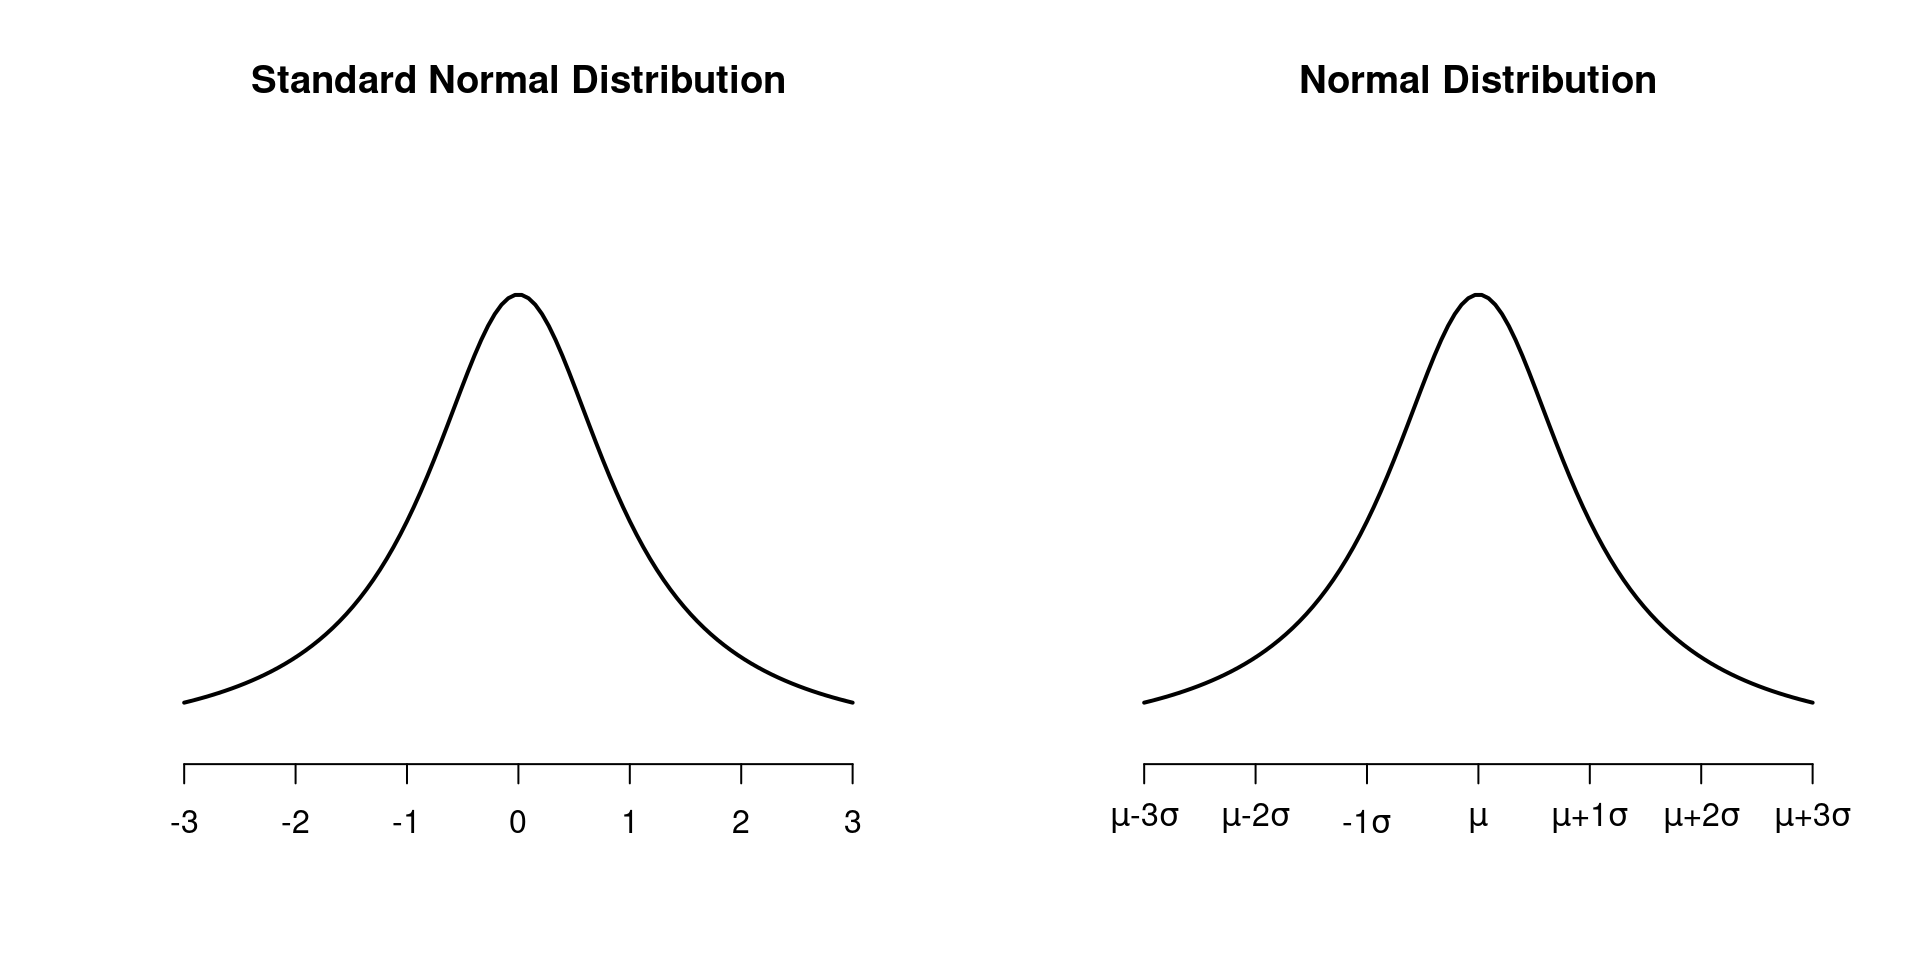
\includegraphics{_main_files/figure-latex/unnamed-chunk-2-1.pdf}

\textbf{Parameters of the Normal distribution}

\fcolorbox{black}{white}{\color{black}
\begin{minipage}[c][6cm][t]{\textwidth}
\sffamily\fboxrule.1em\fboxsep1em
Q: What are the parameters of the standard normal distribution? Left hand plot.
\\
\\
Q: What are the parameters of a generic normal distribution? Right hand plot.\\
\\
\\
Q: Explain what they mean.
\end{minipage}}

The Normal (Gaussian) is typically used for tests and inference when the variance of a sample is known (but the mean isn't). However this is typically \emph{not} the case

\hypertarget{the-student-t-distribution}{%
\subsection{The Student-T distribution}\label{the-student-t-distribution}}

The Student-T is used to model Normally distributed data when we do not know the mean or the variance. This is the most common situation. The Student-T has one parameter: the degrees of freedom (typically the sample size-2). In most of the tests we conduct we have to estimate the variance from the data and so we can't formally use the Normal distribution but have to use the Student-T. In practice as we use \texttt{R} we don't actually need to worry about the details.

However for our purposes (understanding tests, p-values and confidence intervals) we can work with the Normal distribution as for a sample over 30 it is a close approximation to the Student-T.

\hypertarget{histograms}{%
\subsection{Histograms}\label{histograms}}

Histograms are a way of looking at how the data behave for continuous variables. They divide the continuous variable into sequential sections (called bins) and display the number of times that the value of the variable falls inside each section.

29 students should have completed the Moodle questionnaire asking for their Height (in cm) and their Gender (Male,Female, Prefer not to say (PNTS).

The histograms for the heights is shown below:

\begin{itemize}
\tightlist
\item
  The x-axis of the histogram represents the range of possible values of height: 140 to 200.
\item
  The bins marked in the plot below are in intervals of:
\item
  The height of the bar in each bin represents the number of times the height falls into that bin: i.e.~the frequency or count {[}how many students have heights between 175 and 180?: {]}
\item
  The y-axis is therefore the number of people in each section -- the count or frequency.
\item
  Sometimes histograms show the probability (count/total) instead
\item
  The histogram is a way to represent the \emph{observed distribution} of the data
\end{itemize}

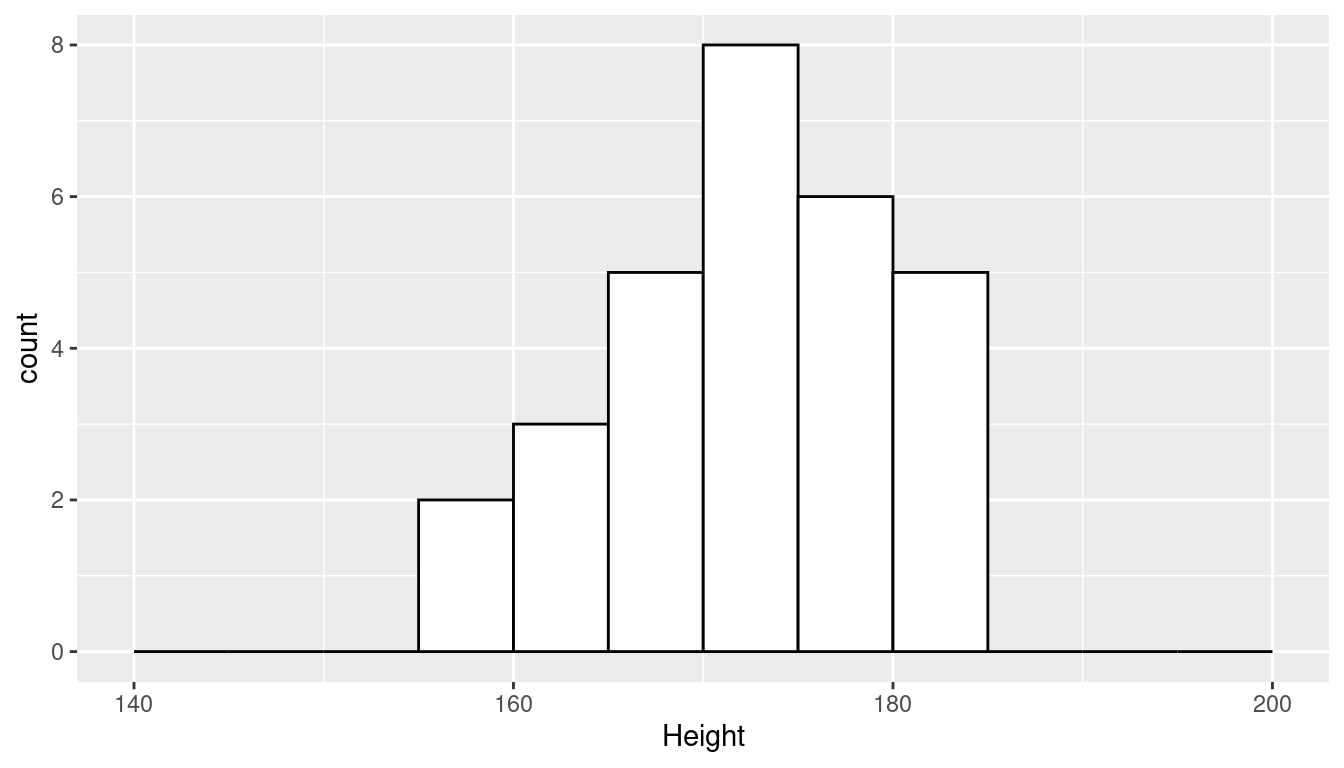
\includegraphics{_main_files/figure-latex/unnamed-chunk-3-1.pdf}

A summary of the heights is given below

\begin{Shaded}
\begin{Highlighting}[]
\FunctionTok{print}\NormalTok{(}\StringTok{"summary"}\NormalTok{)}
\end{Highlighting}
\end{Shaded}

\begin{verbatim}
## [1] "summary"
\end{verbatim}

\begin{Shaded}
\begin{Highlighting}[]
\FunctionTok{summary}\NormalTok{(df}\SpecialCharTok{$}\NormalTok{Height)}
\end{Highlighting}
\end{Shaded}

\begin{verbatim}
##    Min. 1st Qu.  Median    Mean 3rd Qu.    Max. 
##   157.0   168.0   175.0   173.2   178.0   185.0
\end{verbatim}

\begin{Shaded}
\begin{Highlighting}[]
\FunctionTok{print}\NormalTok{(}\StringTok{"sd"}\NormalTok{)}
\end{Highlighting}
\end{Shaded}

\begin{verbatim}
## [1] "sd"
\end{verbatim}

\begin{Shaded}
\begin{Highlighting}[]
\FunctionTok{sd}\NormalTok{(df}\SpecialCharTok{$}\NormalTok{Height)}
\end{Highlighting}
\end{Shaded}

\begin{verbatim}
## [1] 7.329339
\end{verbatim}

\begin{Shaded}
\begin{Highlighting}[]
\CommentTok{\#plot(seq(140,190,by=5),seq(140,190,by=5),col="0",xlab="height (cm)", ylab="frequency",axes=FALSE)}
\CommentTok{\#quantile(df2$height, p=c(0.025,0.975))}
\end{Highlighting}
\end{Shaded}

\begin{itemize}
\tightlist
\item
  The average height of students at the LSE is: 168 cm\\
\item
  with \emph{known} standard error: 7cm\\
\item
  The average height of students in this class is:
\item
  with \emph{estimated} standard error:
\end{itemize}

Overlay a normal distribution with mean and standard deviation of LSE students.

\hypertarget{questions}{%
\subsubsection{Questions:}\label{questions}}

What questions can we ask about the heights of students?

First we want to know whether the height of students from the last 2 years of ST211 is the same (on average) as that of LSE students.

\fcolorbox{black}{white}{\color{black}
\begin{minipage}[c][4cm][t]{\textwidth}
\sffamily\fboxrule.1em\fboxsep1em
Q: Based on the statistics above, do you think the distribution of students at the LSE is a good match for the height of students in this class? Compare:\\

* The averages\\
* The spread
\end{minipage}}

\hypertarget{one-sample-z-tests}{%
\subsubsection{One sample z-tests}\label{one-sample-z-tests}}

\begin{itemize}
\tightlist
\item
  We're going to make an unrealistic assumption for the sake of simplicity. The two variances above for all LSE students and those in this class are close enough so we'll assume that they are the same and that therefore the variance of height of students in this class is \emph{known} to be:
\item
  This means that we only need to look estimate \emph{one} mean
\item
  \emph{If the averages are the same that means that the difference between them must be 0}
\end{itemize}

\hypertarget{hypothesis-test}{%
\subsection{Hypothesis test}\label{hypothesis-test}}

Formally the we talk about hypotheses for statistical tests. In this case

\begin{itemize}
\tightlist
\item
  The \emph{null} hypothesis: There is no difference in the means \(\mu_{class}-\mu_{LSE}=0\)
\item
  The \emph{alternative} hypothesis: There is a difference between them \(\mu_{class}-\mu_{LSE} \neq 0\)
\end{itemize}

\textbf{Formula for the z-statistic}

\fcolorbox{black}{white}{\color{black}
\begin{minipage}[c][4cm][t]{\textwidth}
\sffamily\fboxrule.1em\fboxsep1em
\color{white}xxxxxxxxxxxx\color{black}
\end{minipage}}

\begin{enumerate}
\def\labelenumi{\arabic{enumi}.}
\tightlist
\item
  We subtract means in the numerator
\item
  We \emph{standardise} in the denominator
\item
  This value is called the \emph{z-statistic}
\item
  We compare it to the standard normal distribution
\end{enumerate}

Intuitively if the absolute value of the z-statistic is very small i.e close to 0 then we can assume that the distribution of our observed heights is the same as that of the LSE student heights. If on the other hand the absolute value is large then it is far from 0 and it becomes harder to assume that the data from this class comes from the LSE student height distribution. The larger the absolute value of the z-statistic the less realistic the null hypothesis.

Somewhat arbitrarily, if the z-statistic exceeds 1.96 in absolute value we say that we have no evidence in favour of the null hypothesis at the 5\% level. This corresponds to the 95\% points. In practice we round this to 2 so we can make quick calculations.

\hypertarget{significance-p-value-and-confidence-intervals}{%
\subsection{Significance, P-value and confidence intervals}\label{significance-p-value-and-confidence-intervals}}

When the z-statistic is within the 95th quantiles then we say that there is \emph{not sufficient evidence to reject the null hypothesis} and that the result is \emph{not statistically significant at the 5\% level}. If the z-statistic exceeds the 95th quantiles then we say there is evidence to reject the null hypothesis and the result is \emph{statistically significant at the 5\% level}.

The \emph{p-value} associated with the test is the probability of observing the value we have or a larger value (in absolute terms): \emph{provided the null hypothesis is true}. If the p-value is smaller than 5\% (0.05) then we say that the result is \emph{statistically significant at the 5\% level}.

Another way of looking at it is to see whether the 95\% \emph{confidence interval} include 0. If it includes 0 then the result is \emph{not statistically significant at the 5\% level}. If the 95\% confidence interval does not include 0 then the result is \emph{statistically significant at the 5\% level}.

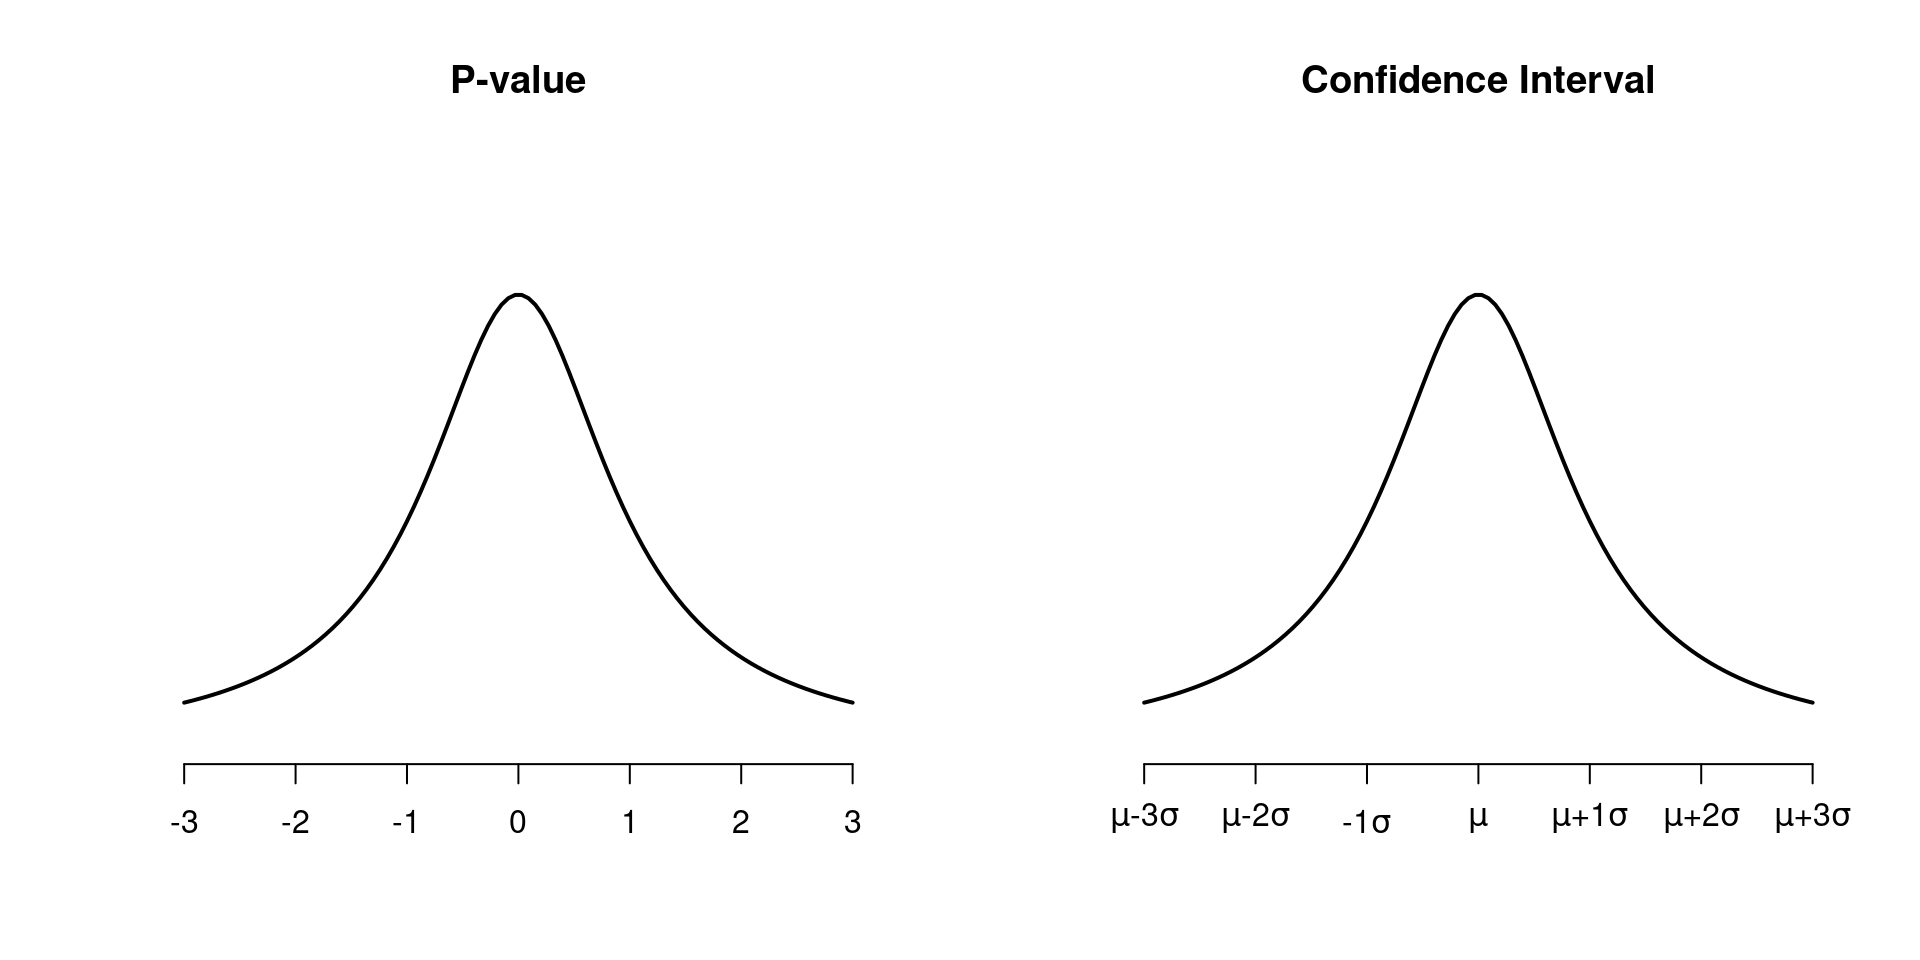
\includegraphics{_main_files/figure-latex/unnamed-chunk-5-1.pdf}

\textbf{Notes}

Typically we focus on the 5\% level of statistical significance for 2-tailed tests. However we could consider different levels such as 1\% or 10\%. In some disciplines 10\% significance is considered the standard. Also, we used a two-tailed tests which means that the 95\% confidence interval is symmetric around the mean and there is 2.5\% on either tail. However for some situations a one tailed test is appropriate. For example if we want to compare two values where the difference can only be 0 or positive it would make sense to do this (e.g.~growth of children).

\hypertarget{two-sample-t-test}{%
\subsection{Two sample T-test:}\label{two-sample-t-test}}

The two sample t-test is similar to the one-sample test we saw above with some important differences:

\begin{enumerate}
\def\labelenumi{\arabic{enumi}.}
\tightlist
\item
  We have to estimate the averages for both samples as they are both unknown
\item
  We have to estimate the variance from the data and therefore use a Student-T distribution
\item
  Typically we assume that the two groups have a common variance (this can be relaxed) and estimate a \emph{pooled standard deviation}
\end{enumerate}

\textbf{Formula for the t-statistic and the pooled standard deviation:}

\fcolorbox{black}{white}{\color{black}
\begin{minipage}[c][6cm][t]{\textwidth}
\sffamily\fboxrule.1em\fboxsep1em
\color{white}xxxxxxxxxxxx\color{black}
\end{minipage}}

We'll apply this to the data on heights where we look at men and women and ask whether their heights can be considered the same:

Males:

\begin{Shaded}
\begin{Highlighting}[]
\FunctionTok{with}\NormalTok{(}\FunctionTok{subset}\NormalTok{(df,Gender}\SpecialCharTok{==}\StringTok{"Male"}\NormalTok{), }\FunctionTok{mean}\NormalTok{(Height))}
\end{Highlighting}
\end{Shaded}

\begin{verbatim}
## [1] 175.4545
\end{verbatim}

\begin{Shaded}
\begin{Highlighting}[]
\FunctionTok{with}\NormalTok{(}\FunctionTok{subset}\NormalTok{(df,Gender}\SpecialCharTok{==}\StringTok{"Male"}\NormalTok{), }\FunctionTok{sd}\NormalTok{(Height))}
\end{Highlighting}
\end{Shaded}

\begin{verbatim}
## [1] 5.396006
\end{verbatim}

Females:

\begin{Shaded}
\begin{Highlighting}[]
\FunctionTok{with}\NormalTok{(}\FunctionTok{subset}\NormalTok{(df,Gender}\SpecialCharTok{==}\StringTok{"Female"}\NormalTok{), }\FunctionTok{mean}\NormalTok{(Height))}
\end{Highlighting}
\end{Shaded}

\begin{verbatim}
## [1] 163.3333
\end{verbatim}

\begin{Shaded}
\begin{Highlighting}[]
\FunctionTok{with}\NormalTok{(}\FunctionTok{subset}\NormalTok{(df,Gender}\SpecialCharTok{==}\StringTok{"Female"}\NormalTok{), }\FunctionTok{sd}\NormalTok{(Height))}
\end{Highlighting}
\end{Shaded}

\begin{verbatim}
## [1] 4.885352
\end{verbatim}

\begin{itemize}
\tightlist
\item
  The average and sd of height of women in this class is:
\item
  The average and sd of height of men in this class is:
\end{itemize}

\fcolorbox{black}{white}{\color{black}
\begin{minipage}[c][4cm][t]{\textwidth}
\sffamily\fboxrule.1em\fboxsep1em

Q: Calculate the (pooled) standard deviation bearing in mind that there are 6 Females, one Prefer not to say and the rest are males. There are 29 students altogether.

\end{minipage}}

Below is the histogram showing men and women. Add two curves to the plot for the heights, one for men and one for women taking into account their means. The formula for the two-sample t-test with common variance is almost exactly the same as the one for the one-sample test and the principle is the same. If the means are the same then the distribution of the difference will be 0.

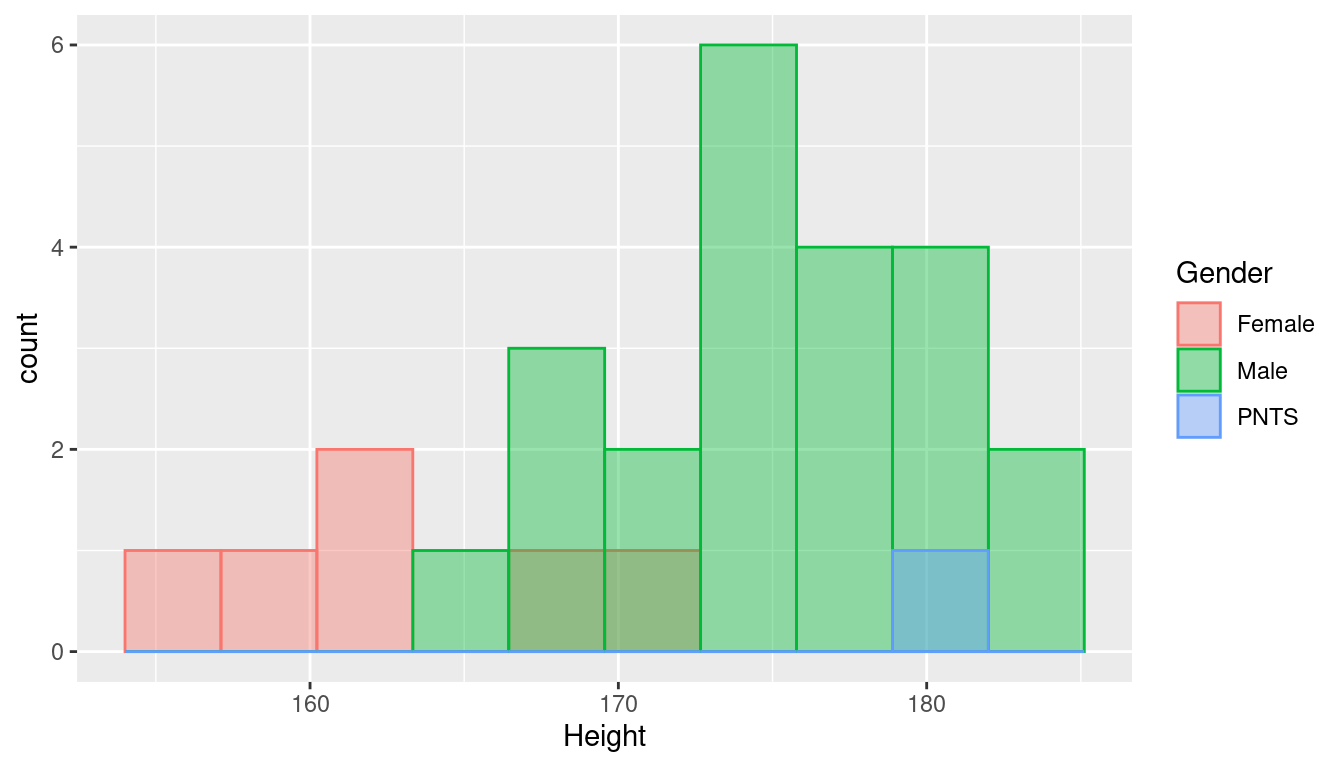
\includegraphics{_main_files/figure-latex/unnamed-chunk-8-1.pdf}

\newpage

\fcolorbox{black}{white}{\color{black}
\begin{minipage}[c][5cm][t]{\textwidth}
\sffamily\fboxrule.1em\fboxsep1em
Q: Calculate the t-statistic bearing in mind that there are 6 Females, one Prefer not to say and the rest are males. There are 29 students altogether.
\end{minipage}}

This value is called the t-statistic and is compared to the Student-T distribution on \(n_w + n_m - 2\) degrees of freedom but we can interpret it in the same way as the z-statistic. Here \(n_w\) is the sample size of women and \(n_m\) is the sample size of men.

\hypertarget{hypothesis-tests}{%
\subsection{Hypothesis tests}\label{hypothesis-tests}}

Formally the we talk about hypothesis tests for statistical tests like the z and the t-tests:

\begin{itemize}
\tightlist
\item
  The \emph{null} hypothesis: There is no difference in the means \(\mu_{m}-\mu_{w}=0\)
\item
  The \emph{alternative} hypothesis: There is a difference between them \(\mu_{m}-\mu_{w} \neq 0\)
\end{itemize}

\fcolorbox{black}{white}{\color{black}
\begin{minipage}[c][4cm][t]{\textwidth}
\sffamily\fboxrule.1em\fboxsep1em
Q: Is the t-statistics we calculated significant at the 5\% level? Why?

\end{minipage}}

You should remember the formulae as you might be asked to calculate a t-statistic in an exam. In practice for our course we get \texttt{R} to do it.

\hypertarget{workshop-1-introduction-to-r-and-rstudio}{%
\section{\texorpdfstring{Workshop 1: Introduction to \texttt{R} and \texttt{RStudio}}{Workshop 1: Introduction to R and RStudio}}\label{workshop-1-introduction-to-r-and-rstudio}}

\hypertarget{learning-objectives}{%
\subsection{Learning objectives}\label{learning-objectives}}

Learn basics of \texttt{R} coding, logical operators as well as vectors and arrays

Familiarise yourself with \texttt{RStudio}

\textbf{LSE PC alert}

The software and PCs in the computer rooms are relatively new and should work well. However please bear in mind that sometimes there are difficulties with the network and/or slightly different PC versions. In this case, please let me know asap although there is typically not a lot I can do immediately.

If you have a laptop that you can easily carry around, I would recommend you use it.

\hypertarget{why-should-i-learn-to-code}{%
\subsection{Why should I learn to code?}\label{why-should-i-learn-to-code}}

Good statisticians learn to program because:

\begin{itemize}
\tightlist
\item
  Independence: Otherwise, you rely on someone else having given you exactly the right tool (although we use many inbuilt \emph{functions} or those developed by other programmers)
\item
  Honesty: Otherwise, you end up distorting your problem to match the tools you have
\item
  Clarity: Making your method is something a machine can do disciplines your thinking and means others can see what you're doing and reproduce it.
\end{itemize}

\hypertarget{how}{%
\subsection{How?}\label{how}}

We'll be learning how to do some programming and using built-in \texttt{R} functions.

\begin{itemize}
\tightlist
\item
  No programming knowledge presumed
\item
  I expect you to know your 1st year stats (although we've been reviewing this).
\item
  I drew heavily on a course by Cosma Shalizi and on Moodle I've put a link to his lectures on \texttt{R} if you want to know more.
\item
  We will not necessarily cover all the material in this section but it is there if you want to use it for reference.
\end{itemize}

\hypertarget{what-now}{%
\subsection{What now?}\label{what-now}}

Today I will briefly go over the \texttt{RStudio} console.

\begin{itemize}
\tightlist
\item
  You will get a chance to practice more during the quiz
\item
  If we don't get through everything I expect you to finish in your own time
\item
  \emph{It is going to be difficult} at the beginning. That is normal.
\item
  You will make mistakes. It will be frustrating.
\item
  It is important for you to read the \emph{errors} you get -- they are not always illuminating but you will come to understand them. There is a reference sheet to common errors and their meaning on Moodle.
\end{itemize}

\hypertarget{rstudio-1}{%
\subsection{\texorpdfstring{\texttt{RStudio}}{RStudio}}\label{rstudio-1}}

Go to the application \(\rightarrow\) Statistics \(\rightarrow\) \texttt{R} \(\rightarrow\)\texttt{RStudio} and open the latest version with the ``full libraries'' option. Then go to File and New File \(\rightarrow\) R script. \texttt{RStudio} allows you to see all parts you use for \texttt{R}:

\begin{itemize}
\tightlist
\item
  \emph{The script}: where you write the \texttt{R} commands that work. You save this so you have a list of working instructions to refer back to -- like a recipe or lego instructions
\item
  \emph{The console}: Basic interaction with \texttt{R} is by typing in the console, a.k.a. terminal or command-line. You type in commands, \texttt{R} runs them and sometimes gives back answers (or errors)
\item
  \emph{The Environment/History tabs} : if you define variables or upload data it shows in the Environment tab. History tab is a list of the commands so far and is useful if you want to figure out which command you used worked
\item
  \emph{The Files/Plots etc tabs} : Files in the local directory, Plots you might be creating, Packages that are installed, Help and viewer. Mostly you will focus on the Files and Plots.
\end{itemize}

\hypertarget{the-working-directory}{%
\subsection{The working directory}\label{the-working-directory}}

The directory you open \texttt{RStudio} from is the working directory. If you want to know where it is and what's in it. Go to the console.

What directory am I in?

\begin{Shaded}
\begin{Highlighting}[]
\FunctionTok{getwd}\NormalTok{()}
\end{Highlighting}
\end{Shaded}

\begin{verbatim}
## [1] "/home/sara/Dropbox (LSE Statistics)/Work_from_Google_Drive/NewR/Gitbook"
\end{verbatim}

What's in it?

\begin{Shaded}
\begin{Highlighting}[]
\FunctionTok{dir}\NormalTok{()}
\end{Highlighting}
\end{Shaded}

\hypertarget{at-the-beginning-of-every-session}{%
\subsection{At the beginning of every session:}\label{at-the-beginning-of-every-session}}

\begin{itemize}
\tightlist
\item
  Open Zoom if you are using it.
\item
  Create a folder/directory named Week x in your H drive. E.g. today you can create a folder called ``Week 1''
\item
  When we use data save all the data files from Moodle into that Week's folder
\item
  Save your \texttt{R} scripts and plots into this file
\item
  To get \texttt{RStudio} to work in this directory you use
\end{itemize}

\texttt{setwd(}\(\color{white}{\text{SOME SPACE HERE FOR STUFF}}\)\texttt{)}
* Or in \texttt{RStudio} go to the \texttt{Files} tab in the bottom right hand corner and navigate to the directory you wand and then under \texttt{More} choose \texttt{Set\ As\ Working\ Directory}.

\hypertarget{data-types}{%
\subsection{Data types}\label{data-types}}

\begin{itemize}
\tightlist
\item
  \emph{Booleans}: Direct binary values: TRUE or FALSE (0,1) in \texttt{R}
\item
  \emph{Integers}: whole numbers: positive, negative or zero
\item
  \emph{Characters}: single letters or symbols, strings = sequences of characters
\item
  \emph{Floating point numbers}: a fraction
\item
  \emph{Missing} or \emph{ill-defined values}: \texttt{NA}, \texttt{NaN}, \texttt{Inf}.
\item
  \emph{numeric} includes both integers and floating point numbers
\end{itemize}

\newpage

\hypertarget{operators}{%
\subsection{Operators}\label{operators}}

Type the examples with me:

\begin{itemize}
\item
  \emph{Binary}: usual arithmetic operators, plus ones for modulo and integer division; take two numbers and give another number

  \begin{longtable}[]{@{}ccl@{}}
  \toprule()
  Operator & Example & What it does \\
  \midrule()
  \endhead
  + & 9+4 & addition \\
  - & 9-4 & subtraction \\
  * & 9*4 & multiplication \\
  / & 9/4 & division \\
  \%/\% & 9\%/\%4 & integer division \\
  \%\% & 9\%\%4 & modulo \\
  \bottomrule()
  \end{longtable}
\item
  \emph{Logical operators} : Comparisons which are also binary operators

  \begin{longtable}[]{@{}ccl@{}}
  \toprule()
  Operator & Example & What it does \\
  \midrule()
  \endhead
  \textgreater{} & 9\textgreater4 & greater than \\
  \textless{} & 9\textless4 & less than \\
  \textgreater= & 9\textgreater=4 & greater or equal \\
  \textless= & 9\textless=4 & smaller or equal \\
  == & 9==4 & equal to \\
  != & 9!=4 & not equal to \\
  \bottomrule()
  \end{longtable}
\item
  \emph{Boolean operators} : ``and'' and ``or''
\end{itemize}

\begin{longtable}[]{@{}ccl@{}}
\toprule()
Operator & Example & What it does \\
\midrule()
\endhead
\& & (9\textgreater4) \& (5\textless6) & are left \emph{and} right true? \\
\textbar{} & (9\textgreater4) \textbar{} (5\textgreater6) & are left \emph{or} right true? \\
\bottomrule()
\end{longtable}

\begin{itemize}
\tightlist
\item
  \emph{Unary}: for arithmetic negation, ! \texttt{x!=y} would give true if x is not equal to y and false otherwise.
\end{itemize}

\hypertarget{checkingimposing-types}{%
\subsection{Checking/Imposing types}\label{checkingimposing-types}}

This can be useful when we don't know what the type of an object is or want to impose a type on an object.

\begin{itemize}
\tightlist
\item
  For asking use \texttt{is.}
\item
  For imposing use \texttt{as.}
\end{itemize}

\begin{longtable}[]{@{}
  >{\raggedright\arraybackslash}p{(\columnwidth - 6\tabcolsep) * \real{0.2034}}
  >{\raggedright\arraybackslash}p{(\columnwidth - 6\tabcolsep) * \real{0.3051}}
  >{\raggedright\arraybackslash}p{(\columnwidth - 6\tabcolsep) * \real{0.1949}}
  >{\raggedright\arraybackslash}p{(\columnwidth - 6\tabcolsep) * \real{0.2966}}@{}}
\toprule()
\begin{minipage}[b]{\linewidth}\raggedright
Example
\end{minipage} & \begin{minipage}[b]{\linewidth}\raggedright
What it does
\end{minipage} & \begin{minipage}[b]{\linewidth}\raggedright
Example
\end{minipage} & \begin{minipage}[b]{\linewidth}\raggedright
What it does (if possible)
\end{minipage} \\
\midrule()
\endhead
\texttt{typeof(9.6)} & what type of variable? & & \\
\texttt{is.numeric(9)} & is the variable a number? & \texttt{as.numeric(TRUE)} & makes the value numeric \\
\texttt{is.integer(6.7)} & is the variable an integer & \texttt{as.integer(6.7)} & turns value into its integer part \\
\texttt{is.character("a")} & is the variable a character/string & \texttt{as.character(6/5)} & makes a string of the number \\
\texttt{is.na(1)} & is the variable an NA & & \\
\bottomrule()
\end{longtable}

See what errors you get when you do things that are not possible.

\begin{Shaded}
\begin{Highlighting}[]
\CommentTok{\#as.integer("a")}
\end{Highlighting}
\end{Shaded}

\hypertarget{data-objects}{%
\subsection{Data objects}\label{data-objects}}

Data objects are the main thing we create, use and manipulate in \texttt{R}. We typically give data objects names. These are then called \emph{variables}. We create them by using the assignment operator \texttt{\textless{}-} (or \texttt{=}). We do this because

\begin{itemize}
\tightlist
\item
  It makes it easier and faster to program
\item
  Easier to debug
\item
  Easier to build functions
\item
  Easier to reuse and understand
\end{itemize}

\begin{Shaded}
\begin{Highlighting}[]
\NormalTok{new.var}\OtherTok{\textless{}{-}}\DecValTok{1}
\NormalTok{new.var}
\end{Highlighting}
\end{Shaded}

\begin{verbatim}
## [1] 1
\end{verbatim}

\begin{Shaded}
\begin{Highlighting}[]
\FunctionTok{exp}\NormalTok{(}\DecValTok{1}\NormalTok{)}
\end{Highlighting}
\end{Shaded}

\begin{verbatim}
## [1] 2.718282
\end{verbatim}

It is also used to change the value of an existing variable

\begin{Shaded}
\begin{Highlighting}[]
\NormalTok{new.var}\OtherTok{\textless{}{-}}\DecValTok{5}
\NormalTok{new.var}\SpecialCharTok{\^{}}\DecValTok{2}
\end{Highlighting}
\end{Shaded}

\begin{verbatim}
## [1] 25
\end{verbatim}

\hypertarget{the-workspaceenvironment}{%
\subsection{The Workspace/Environment}\label{the-workspaceenvironment}}

Look at the Environment tab on the top right of \texttt{RStudio}. Can you see new.var?

\begin{verbatim}
## [1] "df"      "df2"     "hx"      "new.var" "x"
\end{verbatim}

Should also just list \texttt{new.var}. If you change the view from list to grid you'll also see that you are given the type of the variable - \texttt{numeric()}.

\hypertarget{vectors}{%
\subsection{Vectors}\label{vectors}}

We can't do much statistics with a single value. Let's group some values together. The simplest \emph{data structure} is the vector:

\begin{Shaded}
\begin{Highlighting}[]
\NormalTok{first.vector}\OtherTok{\textless{}{-}}\FunctionTok{c}\NormalTok{(}\DecValTok{1}\NormalTok{,}\DecValTok{7}\NormalTok{,}\DecValTok{11}\NormalTok{,}\DecValTok{43}\NormalTok{)}
\NormalTok{first.vector}
\end{Highlighting}
\end{Shaded}

\begin{verbatim}
## [1]  1  7 11 43
\end{verbatim}

\begin{Shaded}
\begin{Highlighting}[]
\FunctionTok{is.vector}\NormalTok{(first.vector)}
\end{Highlighting}
\end{Shaded}

\begin{verbatim}
## [1] TRUE
\end{verbatim}

The \texttt{c()} function creates a vector with the values in the order specified. Some things you can do to vectors

\begin{Shaded}
\begin{Highlighting}[]
\FunctionTok{length}\NormalTok{(first.vector)}
\end{Highlighting}
\end{Shaded}

\begin{verbatim}
## [1] 4
\end{verbatim}

\begin{Shaded}
\begin{Highlighting}[]
\NormalTok{first.vector}\SpecialCharTok{+}\DecValTok{1}
\end{Highlighting}
\end{Shaded}

\begin{verbatim}
## [1]  2  8 12 44
\end{verbatim}

\begin{Shaded}
\begin{Highlighting}[]
\NormalTok{first.vector}\SpecialCharTok{*}\DecValTok{2}
\end{Highlighting}
\end{Shaded}

\begin{verbatim}
## [1]  2 14 22 86
\end{verbatim}

\begin{Shaded}
\begin{Highlighting}[]
\NormalTok{first.vector}\SpecialCharTok{\^{}}\DecValTok{2}
\end{Highlighting}
\end{Shaded}

\begin{verbatim}
## [1]    1   49  121 1849
\end{verbatim}

More things

\begin{Shaded}
\begin{Highlighting}[]
\NormalTok{second.vector}\OtherTok{\textless{}{-}}\FunctionTok{c}\NormalTok{(}\DecValTok{1}\NormalTok{,}\DecValTok{2}\NormalTok{,}\DecValTok{1}\NormalTok{,}\DecValTok{2}\NormalTok{)}
\NormalTok{first.vector}\SpecialCharTok{+}\NormalTok{second.vector}
\end{Highlighting}
\end{Shaded}

\begin{verbatim}
## [1]  2  9 12 45
\end{verbatim}

\begin{Shaded}
\begin{Highlighting}[]
\NormalTok{first.vector}\SpecialCharTok{\^{}}\NormalTok{second.vector}
\end{Highlighting}
\end{Shaded}

\begin{verbatim}
## [1]    1   49   11 1849
\end{verbatim}

\begin{Shaded}
\begin{Highlighting}[]
\NormalTok{first.vector}\SpecialCharTok{\textgreater{}}\NormalTok{second.vector}
\end{Highlighting}
\end{Shaded}

\begin{verbatim}
## [1] FALSE  TRUE  TRUE  TRUE
\end{verbatim}

To compare vectors use \texttt{identical} or \texttt{all.equal}

\begin{Shaded}
\begin{Highlighting}[]
\FunctionTok{identical}\NormalTok{(first.vector,}\FunctionTok{c}\NormalTok{(}\DecValTok{1}\NormalTok{,}\DecValTok{7}\NormalTok{,}\DecValTok{11}\NormalTok{,}\DecValTok{43}\NormalTok{))}
\end{Highlighting}
\end{Shaded}

\begin{verbatim}
## [1] TRUE
\end{verbatim}

\begin{Shaded}
\begin{Highlighting}[]
\FunctionTok{identical}\NormalTok{(}\FunctionTok{c}\NormalTok{(}\FloatTok{0.3{-}0.1}\NormalTok{,}\DecValTok{0}\NormalTok{),}\FunctionTok{c}\NormalTok{(}\FloatTok{0.4{-}0.2}\NormalTok{,}\DecValTok{0}\NormalTok{))}
\end{Highlighting}
\end{Shaded}

\begin{verbatim}
## [1] FALSE
\end{verbatim}

\begin{Shaded}
\begin{Highlighting}[]
\FunctionTok{all.equal}\NormalTok{(}\FunctionTok{c}\NormalTok{(}\FloatTok{0.3{-}0.1}\NormalTok{,}\DecValTok{0}\NormalTok{),}\FunctionTok{c}\NormalTok{(}\FloatTok{0.4{-}0.2}\NormalTok{,}\DecValTok{0}\NormalTok{))}
\end{Highlighting}
\end{Shaded}

\begin{verbatim}
## [1] TRUE
\end{verbatim}

\hypertarget{extracting-parts-of-vectors}{%
\subsection{Extracting parts of vectors}\label{extracting-parts-of-vectors}}

If you want the 2nd value of your vector

\begin{Shaded}
\begin{Highlighting}[]
\NormalTok{first.vector[}\DecValTok{2}\NormalTok{]}
\end{Highlighting}
\end{Shaded}

\begin{verbatim}
## [1] 7
\end{verbatim}

If you want the 2nd and 4th or the 2nd \emph{to} the 4th

\begin{Shaded}
\begin{Highlighting}[]
\NormalTok{first.vector[}\FunctionTok{c}\NormalTok{(}\DecValTok{2}\NormalTok{,}\DecValTok{4}\NormalTok{)]}
\end{Highlighting}
\end{Shaded}

\begin{verbatim}
## [1]  7 43
\end{verbatim}

\begin{Shaded}
\begin{Highlighting}[]
\NormalTok{first.vector[}\DecValTok{2}\SpecialCharTok{:}\DecValTok{4}\NormalTok{]}
\end{Highlighting}
\end{Shaded}

\begin{verbatim}
## [1]  7 11 43
\end{verbatim}

If you want the vector \emph{without} the 1st and 3rd

\begin{Shaded}
\begin{Highlighting}[]
\NormalTok{first.vector[}\FunctionTok{c}\NormalTok{(}\SpecialCharTok{{-}}\DecValTok{1}\NormalTok{,}\SpecialCharTok{{-}}\DecValTok{3}\NormalTok{)]}
\end{Highlighting}
\end{Shaded}

\begin{verbatim}
## [1]  7 43
\end{verbatim}

Say you want the values that are larger than 8

\begin{Shaded}
\begin{Highlighting}[]
\NormalTok{first.vector[first.vector}\SpecialCharTok{\textgreater{}}\DecValTok{8}\NormalTok{]}
\end{Highlighting}
\end{Shaded}

\begin{verbatim}
## [1] 11 43
\end{verbatim}

Say you want to know the position in the vector (the \emph{index}) of the values that are larger than 8

\begin{Shaded}
\begin{Highlighting}[]
\FunctionTok{which}\NormalTok{(first.vector}\SpecialCharTok{\textgreater{}}\DecValTok{8}\NormalTok{)}
\end{Highlighting}
\end{Shaded}

\begin{verbatim}
## [1] 3 4
\end{verbatim}

\begin{Shaded}
\begin{Highlighting}[]
\NormalTok{first.vector[}\FunctionTok{which}\NormalTok{(first.vector}\SpecialCharTok{\textgreater{}}\DecValTok{8}\NormalTok{)]}
\end{Highlighting}
\end{Shaded}

\begin{verbatim}
## [1] 11 43
\end{verbatim}

\hypertarget{arrays}{%
\subsection{Arrays}\label{arrays}}

Let's make an array with 2 rows by 2 columns using our \texttt{first.vector}

\begin{Shaded}
\begin{Highlighting}[]
\NormalTok{first.array}\OtherTok{\textless{}{-}}\FunctionTok{array}\NormalTok{(first.vector,}\AttributeTok{dim=}\FunctionTok{c}\NormalTok{(}\DecValTok{2}\NormalTok{,}\DecValTok{2}\NormalTok{))}
\NormalTok{first.array}
\end{Highlighting}
\end{Shaded}

\begin{verbatim}
##      [,1] [,2]
## [1,]    1   11
## [2,]    7   43
\end{verbatim}

Can have any size array.

\begin{Shaded}
\begin{Highlighting}[]
\NormalTok{second.array}\OtherTok{\textless{}{-}}\FunctionTok{array}\NormalTok{(first.vector,}\AttributeTok{dim=}\FunctionTok{c}\NormalTok{(}\DecValTok{4}\NormalTok{,}\DecValTok{2}\NormalTok{))}
\NormalTok{second.array}
\end{Highlighting}
\end{Shaded}

\begin{verbatim}
##      [,1] [,2]
## [1,]    1    1
## [2,]    7    7
## [3,]   11   11
## [4,]   43   43
\end{verbatim}

How big is the array?

\begin{Shaded}
\begin{Highlighting}[]
\FunctionTok{dim}\NormalTok{(first.array)}
\end{Highlighting}
\end{Shaded}

\begin{verbatim}
## [1] 2 2
\end{verbatim}

Like with vectors we might want to know about individual elements of the array. See what the commands below do.

\begin{Shaded}
\begin{Highlighting}[]
\NormalTok{first.array[}\DecValTok{2}\NormalTok{,}\DecValTok{2}\NormalTok{]}
\end{Highlighting}
\end{Shaded}

\begin{verbatim}
## [1] 43
\end{verbatim}

\begin{Shaded}
\begin{Highlighting}[]
\NormalTok{first.array[}\DecValTok{2}\NormalTok{,]}
\end{Highlighting}
\end{Shaded}

\begin{verbatim}
## [1]  7 43
\end{verbatim}

\begin{Shaded}
\begin{Highlighting}[]
\NormalTok{first.array[}\DecValTok{2}\NormalTok{,,drop}\OtherTok{=}\ConstantTok{FALSE}\NormalTok{]}
\end{Highlighting}
\end{Shaded}

\begin{verbatim}
##      [,1] [,2]
## [1,]    7   43
\end{verbatim}

\begin{Shaded}
\begin{Highlighting}[]
\NormalTok{first.array[,}\DecValTok{2}\NormalTok{]}
\end{Highlighting}
\end{Shaded}

\begin{verbatim}
## [1] 11 43
\end{verbatim}

Some commands will preserve the array structure

\begin{Shaded}
\begin{Highlighting}[]
\NormalTok{first.array}\SpecialCharTok{\textgreater{}}\DecValTok{8}
\end{Highlighting}
\end{Shaded}

\begin{verbatim}
##       [,1] [,2]
## [1,] FALSE TRUE
## [2,] FALSE TRUE
\end{verbatim}

\textbf{Vector Recycling}

If a row is longer than the vector that has been assigned to it, \texttt{R} will recycle the vector

\begin{Shaded}
\begin{Highlighting}[]
\NormalTok{another.array}\OtherTok{\textless{}{-}}\FunctionTok{array}\NormalTok{(}\AttributeTok{dim=}\FunctionTok{c}\NormalTok{(}\DecValTok{4}\NormalTok{,}\DecValTok{2}\NormalTok{)) }\CommentTok{\#another array }
\NormalTok{another.array[,}\DecValTok{1}\NormalTok{]}\OtherTok{\textless{}{-}}\FunctionTok{c}\NormalTok{(}\DecValTok{1}\NormalTok{,}\DecValTok{2}\NormalTok{)}
\NormalTok{another.array[,}\DecValTok{2}\NormalTok{]}\OtherTok{\textless{}{-}}\FunctionTok{c}\NormalTok{(}\DecValTok{3}\NormalTok{,}\DecValTok{4}\NormalTok{)}
\NormalTok{another.array}
\end{Highlighting}
\end{Shaded}

\begin{verbatim}
##      [,1] [,2]
## [1,]    1    3
## [2,]    2    4
## [3,]    1    3
## [4,]    2    4
\end{verbatim}

\hypertarget{functions}{%
\subsection{Functions}\label{functions}}

A \emph{function} in \texttt{R} is a command that takes \emph{arguments} and returns an \emph{output}. A function works as follows: you type

\texttt{name.of.function(argument)}

and press enter then you will get the output of the function.

\textbf{Example}

\begin{Shaded}
\begin{Highlighting}[]
\FunctionTok{which}\NormalTok{(first.array}\SpecialCharTok{\textgreater{}}\DecValTok{8}\NormalTok{)}
\end{Highlighting}
\end{Shaded}

\begin{verbatim}
## [1] 3 4
\end{verbatim}

Some functions will return vectors when applied to arrays if you don't set additional options. If you use \texttt{which()} with \texttt{arr.ind=TRUE} then it gives you the locations of the TRUE.

\begin{Shaded}
\begin{Highlighting}[]
\FunctionTok{which}\NormalTok{(first.array}\SpecialCharTok{\textgreater{}}\DecValTok{8}\NormalTok{,}\AttributeTok{arr.ind=}\ConstantTok{TRUE}\NormalTok{)}
\end{Highlighting}
\end{Shaded}

\begin{verbatim}
##      row col
## [1,]   1   2
## [2,]   2   2
\end{verbatim}

Compare this to the output of \texttt{first.array\textgreater{}8}

The homework this week is to work through some code that teaches you about loops and functions in \texttt{R}

\hypertarget{history}{%
\subsection{History}\label{history}}

Have a look at your History tab. It contains ALL the commands you've typed so far (including the wrong ones). If you want to save your commands then it is easy to just save the History. You can remove individual commands by highlighting and clicking on the page with the red cross at the top of the tab.

\hypertarget{packages}{%
\subsection{Packages}\label{packages}}

Packages typically contain a number of (often related) functions to do things in \texttt{R}. One of the great things about \texttt{R} is that you can write your own functions but also you can often find a function someone else has written to do almost anything you need to do. Because \texttt{R} is open source you can access the code of any function anyone has written and modify it if you want. There are hundreds of packages. Go to the \texttt{R} website to search for packages or search via the packages tab in \texttt{RStudio}.

When we first open \texttt{RStudio} it has only a few packages loaded. Look under the the \texttt{Packages} tab in the bottom right hand corner of \texttt{RStudio} to see what's packages are installed. You load a package by typing \texttt{library(nameofpackage)} or by ticking the box next to the name of the package you want in the packages tab.

An important point is that \texttt{R} on the LSE PCs has all the relevant packages installed when you log in as you because it has been set up specially. So you should be able to load the packages without having to install them. Don't try to install anything as this can sometimes lead to crashes. If you install \texttt{R} on your laptop you'll have to install everything yourself. Use the install button in the \texttt{Packages} tab. If you encounter problems with some of the packages let me know asap and I can come up with alternatives.

\hypertarget{at-the-end-of-every-workshop}{%
\subsection{At the end of every Workshop}\label{at-the-end-of-every-workshop}}

\begin{itemize}
\tightlist
\item
  Save the \texttt{R} script in the working directory
\item
  Save any plots in the working directory (use the ``Export'' tab)
\item
  When you close \texttt{RStudio} it will prompt you asking if you want to save the \texttt{.Data} file. This is the ``image'' which contains all the variables, data and functions you have created during the session. It does \emph{not} contain the script i.e.~the set of instructions you typed, only the stuff you created.
\item
  It is worth saving the image if

  \begin{itemize}
  \tightlist
  \item
    You will continue to work on the same project later
  \item
    If the script takes a while to run and it is easier just to save the complex/large objects you have created
  \item
    If you have manipulated the data in complex ways (in this case also save the data in a new data file)
  \item
    If you intend to share your script with others it is important that it will run with an empty session -- passing them the image will help with that.
  \end{itemize}
\end{itemize}

\hypertarget{lecture-2-plots-needed-for-regression}{%
\section{Lecture 2: Plots needed for Regression}\label{lecture-2-plots-needed-for-regression}}

\hypertarget{learning-outcomes-1}{%
\subsection{Learning outcomes}\label{learning-outcomes-1}}

To become familiar with different types variables involved in regression

Reminder of boxplots and scatterplots

Introduction to Q-Q plots

\hypertarget{the-aims-of-regression}{%
\subsection{The aims of regression}\label{the-aims-of-regression}}

The principal aims of regression are to use observed data and maths to create models to:

\begin{enumerate}
\def\labelenumi{\arabic{enumi}.}
\tightlist
\item
  Better \emph{understand} and \emph{explain} the relationships between different factors or variables
\item
  To \emph{predict} the values of a variable of interest based on information currently available
\item
  A combination of the above
\end{enumerate}

In order to do this we need to be able to classify data into \emph{roles} and \emph{types}.

\hypertarget{roles-and-types-of-variables}{%
\subsection{Roles and types of variables}\label{roles-and-types-of-variables}}

In regression we have two main roles for the variables:

\begin{itemize}
\tightlist
\item
  The \emph{outcome} variable

  \begin{itemize}
  \tightlist
  \item
    what we are interested in understanding or predicting. Also called dependent or response variable. We only deal with one outcome in this course, however the theory has been extended to multiple outcomes.
  \end{itemize}
\item
  The \emph{predictor} variable(s)

  \begin{itemize}
  \tightlist
  \item
    what we use to predict or explain the outcome variable. Also called explanatory, independent variable or factor
  \end{itemize}
\end{itemize}

\hypertarget{example-1}{%
\subsubsection{\texorpdfstring{\emph{Example 1}:}{Example 1:}}\label{example-1}}

\begin{itemize}
\tightlist
\item
  \emph{We are given data on 4 different variables for a random sample of 100 staff at the LSE: height (in cm), age (in years), annual income (in 1000's £) and gender (male/female/other)}
\end{itemize}

What is the aim, prediction or explanation? Which variable is the outcome?

\fcolorbox{black}{white}{\color{black}
\begin{minipage}[c][1.5cm][t]{\textwidth}
\sffamily\fboxrule.1em\fboxsep1em
Aim:\\
\\
Outcome variable:\\
\end{minipage}}

\hypertarget{type-of-variable}{%
\subsection{Type of variable}\label{type-of-variable}}

The type of the variable can also be different.

\begin{itemize}
\tightlist
\item
  \emph{Binary} : these have two values only -- 0,1 ; on,off ; Yes,No
\item
  \emph{Categorical} : these have a finite number of values (levels) such that the difference between any two values isn't the same for any pair of values. They are typically qualitative -- country, political party, degree. Some have a natural ordering (e.g.~degree levels) and could be considered as \emph{Ordinal} but we do not make this difference in the course.
\item
  \emph{Numeric} : these are variables which can take any numerical value. Some common variables are rounded to an integer (e.g.~age) or cannot really take on any possible value (\% in an exam). Some are discrete integer values (e.g.~age in years) others are continuous with fractions or decimal places (e.g.~temperature to two decimal places). The key for numeric variables is that the difference between two consecutive values of a variable is the same regardless of which two consecutive values we take.
\end{itemize}

For \emph{Example 1} identify the type of each variable. Justify your answers.

\fcolorbox{black}{white}{\color{black}
\begin{minipage}[c][4cm][t]{\textwidth}
\sffamily\fboxrule.1em\fboxsep1em
\color{white}xxxxxxxxxxxx\color{black}
\end{minipage}}

\hypertarget{how-are-the-variables-related}{%
\subsection{How are the variables related?}\label{how-are-the-variables-related}}

It is very important when encountering a new data set to ask yourself what relationships you \emph{expect to see} between the variables; in particular the outcome and the predictors. You need to think both in terms of sign (+/-) and in terms of strength (is the outcome strongly related to the predictor or is it a weak relationship).

Sometimes you will have no idea! In this case you will hopefully have an expert in the subject matter working with you giving you hints. At other times you will find the sign/importance of a variable diminish when you introduce more variables into a regression. For example, having a bike/car accident may be strongly associated with having severe injuries for the cyclist. If however you include wearing a helmet then this association changes because conditional on wearing a helmet the injuries are less severe.

Thinking about the relationships between variables \emph{before} running the analysis is important for a number of reasons:

\begin{itemize}
\tightlist
\item
  Helps you spot quickly if you need to take a closer look at unexpected results.
\item
  Gives you a deeper understanding of underlying relationships because you have to find ways to explain counter-intuitive results.
\item
  It makes you think more carefully about what the variables are -- the unit, the range etc. E.g. if you have data on height and age you might assume that age and height are correlated until you see that the data are for adults only.
\item
  Is helpful when assessing the modelling assumptions (more of that later).
\end{itemize}

For \emph{Example 1} what do you think the relationships between the outcome and the predictors are? Are any of the predictors likely to be related? Justify your answer.

\fcolorbox{black}{white}{\color{black}
\begin{minipage}[c][4cm][t]{\textwidth}
\sffamily\fboxrule.1em\fboxsep1em
\color{white}xxxxxxxxxxxx\color{black}
\end{minipage}}

\newpage

\hypertarget{exercise}{%
\subsection{Exercise}\label{exercise}}

Identify the outcome and the predictors in the following 2 examples. Try and guess at whether the aim of the research is to explain or predict. Do you anticipate that any of the predictors are associated with one another?

\emph{Example 2}:

\begin{itemize}
\tightlist
\item
  We are given data on the height (in cms to the shoulder), the breed (Ryeland, Romney, Masham) and weight (in kgs) of wool obtained after shearing of 30 sheep belonging to Farmer Josephine. She has a total of 213 sheep.
\end{itemize}

What is the aim, prediction or explanation? Which variable is the outcome?

\fcolorbox{black}{white}{\color{black}
\begin{minipage}[c][1.5cm][t]{\textwidth}
\sffamily\fboxrule.1em\fboxsep1em
Aim:\\
\\
Outcome variable:\\
\end{minipage}}

Identify the type of each variable.

\fcolorbox{black}{white}{\color{black}
\begin{minipage}[c][6cm][t]{\textwidth}
\sffamily\fboxrule.1em\fboxsep1em
\color{white}xxxxxxxxxxxx\color{black}
\end{minipage}}

What do you think the relationships between the outcome and the predictors are? Are any of the predictors likely to be related? Justify your answer.

\fcolorbox{black}{white}{\color{black}
\begin{minipage}[c][6cm][t]{\textwidth}
\sffamily\fboxrule.1em\fboxsep1em
\color{white}xxxxxxxxxxxx\color{black}
\end{minipage}}

\newpage

\emph{Example 3}:

\begin{itemize}
\tightlist
\item
  The data are for a sample of 1000 Londoners who were asked whether they voted (yes/no) in the last general elections, their annual income (in bands 0-20k,20k-30k,30k-40k,40k-50k,50k-60k,60k+), gender (male/female/other), the highest level of education (none/secondary school/university/other) and where in London they live (first two letters of postcode)
\end{itemize}

What is the aim, prediction or explanation? Which variable is the outcome?

\fcolorbox{black}{white}{\color{black}
\begin{minipage}[c][1.5cm][t]{\textwidth}
\sffamily\fboxrule.1em\fboxsep1em
Aim:\\
\\
Outcome variable:\\
\end{minipage}}

Identify the type of each variable. Justify your answers.

\fcolorbox{black}{white}{\color{black}
\begin{minipage}[c][6cm][t]{\textwidth}
\sffamily\fboxrule.1em\fboxsep1em
\color{white}xxxxxxxxxxxx\color{black}
\end{minipage}}

What do you think the relationships between the outcome and the predictors are? Are any of the predictors likely to be related? Justify your answer.

\newpage

\hypertarget{plots}{%
\subsection{Plots}\label{plots}}

There are two types of plots that you'll use regularly in exploratory analysis: \emph{scatterplots} and \emph{boxplots}. We'll quickly review what they show. As we will use Q-Q plots in residual analysis later on we'll introduce them here.

\hypertarget{scatterplots}{%
\subsection{Scatterplots}\label{scatterplots}}

Scatterplots should be used to plot \emph{continuous} predictors against \emph{continuous} outcomes. Examples include:

\begin{itemize}
\tightlist
\item
  age (years) vs income (in £)
\item
  skill score (special unit) vs exam grade (in \%)
\item
  height (cm) vs income (in £)
\item
  shoulder height (cm) vs weight of wool (in kg) in sheep (see below)
\end{itemize}

The predictor is in the x-axis and the outcome is in the y-axis.
\(\\\)

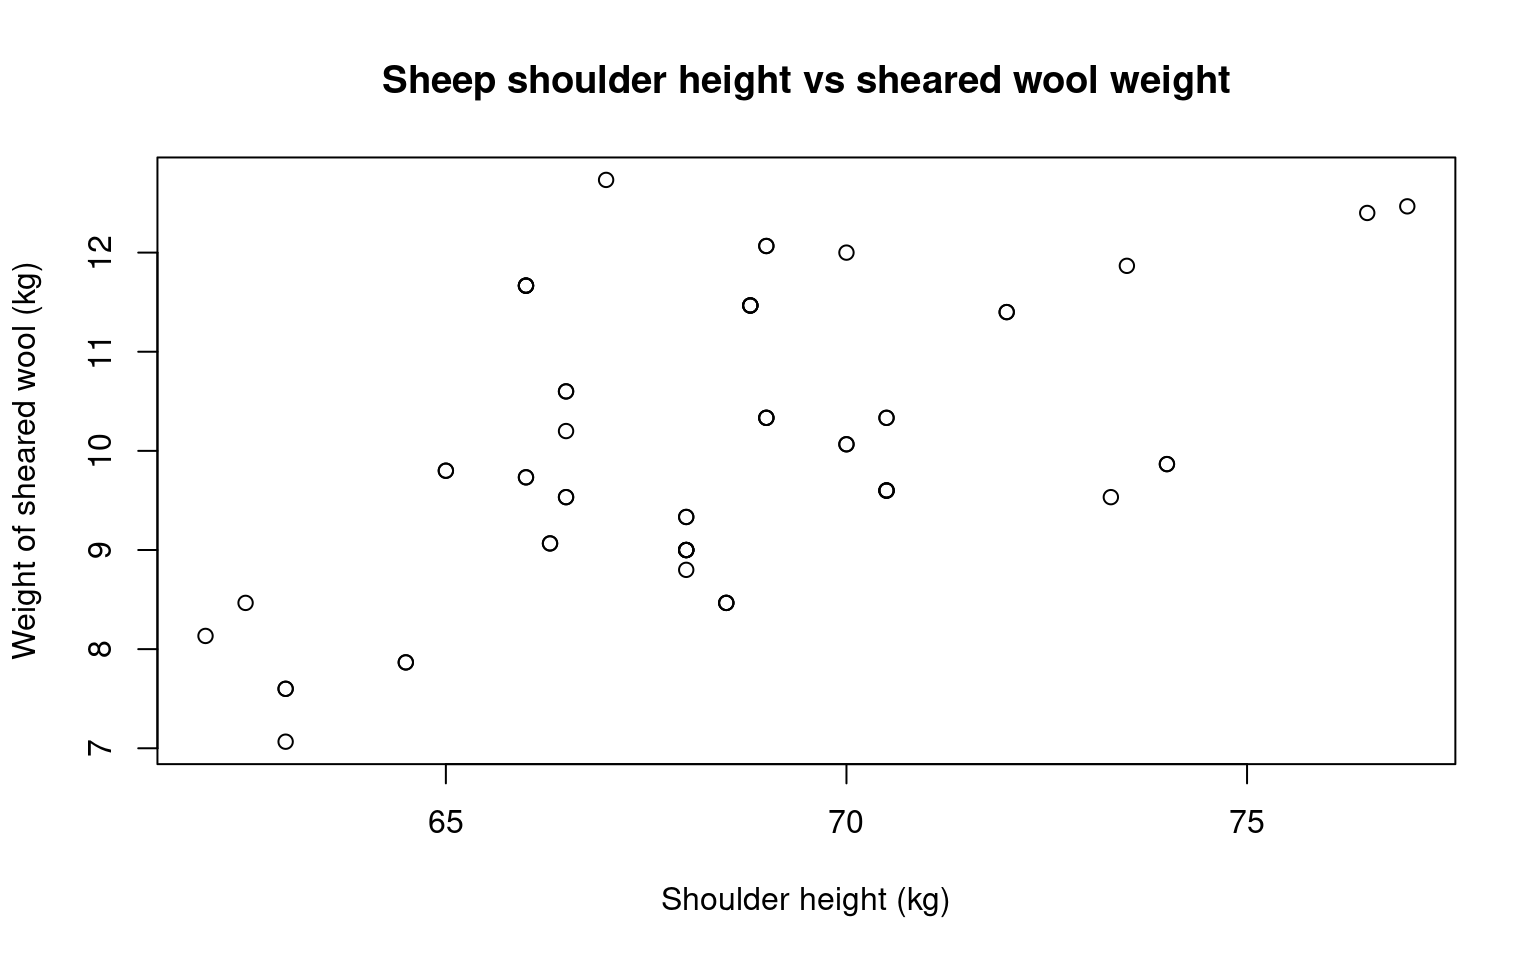
\includegraphics{_main_files/figure-latex/unnamed-chunk-32-1.pdf}

Scatterplots can be used to visually assess

\begin{itemize}
\tightlist
\item
  whether a linear relationship between predictors and outcome is plausible,
\item
  whether there is any non-linearity (i.e.~curvature) in the relationship and
\item
  to get feeling of the strength of the association.
\end{itemize}

Assess the scatterplot above:

\fcolorbox{black}{white}{\color{black}
\begin{minipage}[c][4cm][t]{\textwidth}
\sffamily\fboxrule.1em\fboxsep1em
Linearity plausible?:\\
\\
Non-linearity likely?:\\
\\
\\
Strong association?:\\
\\
\\
\end{minipage}}

\hypertarget{boxplots}{%
\subsection{Boxplots}\label{boxplots}}

Boxplots are used to show the relationship between a \emph{categorical} predictor and a \emph{continuous} outcome.

Examples include:

\begin{itemize}
\tightlist
\item
  Gender (male, female) vs income (in £)
\item
  Political affiliation (Tory, Labour, Lib Dem, Other) vs age (in years)
\item
  Time spent on social media (in hour bands per week) vs exam grade (in \%)
\end{itemize}

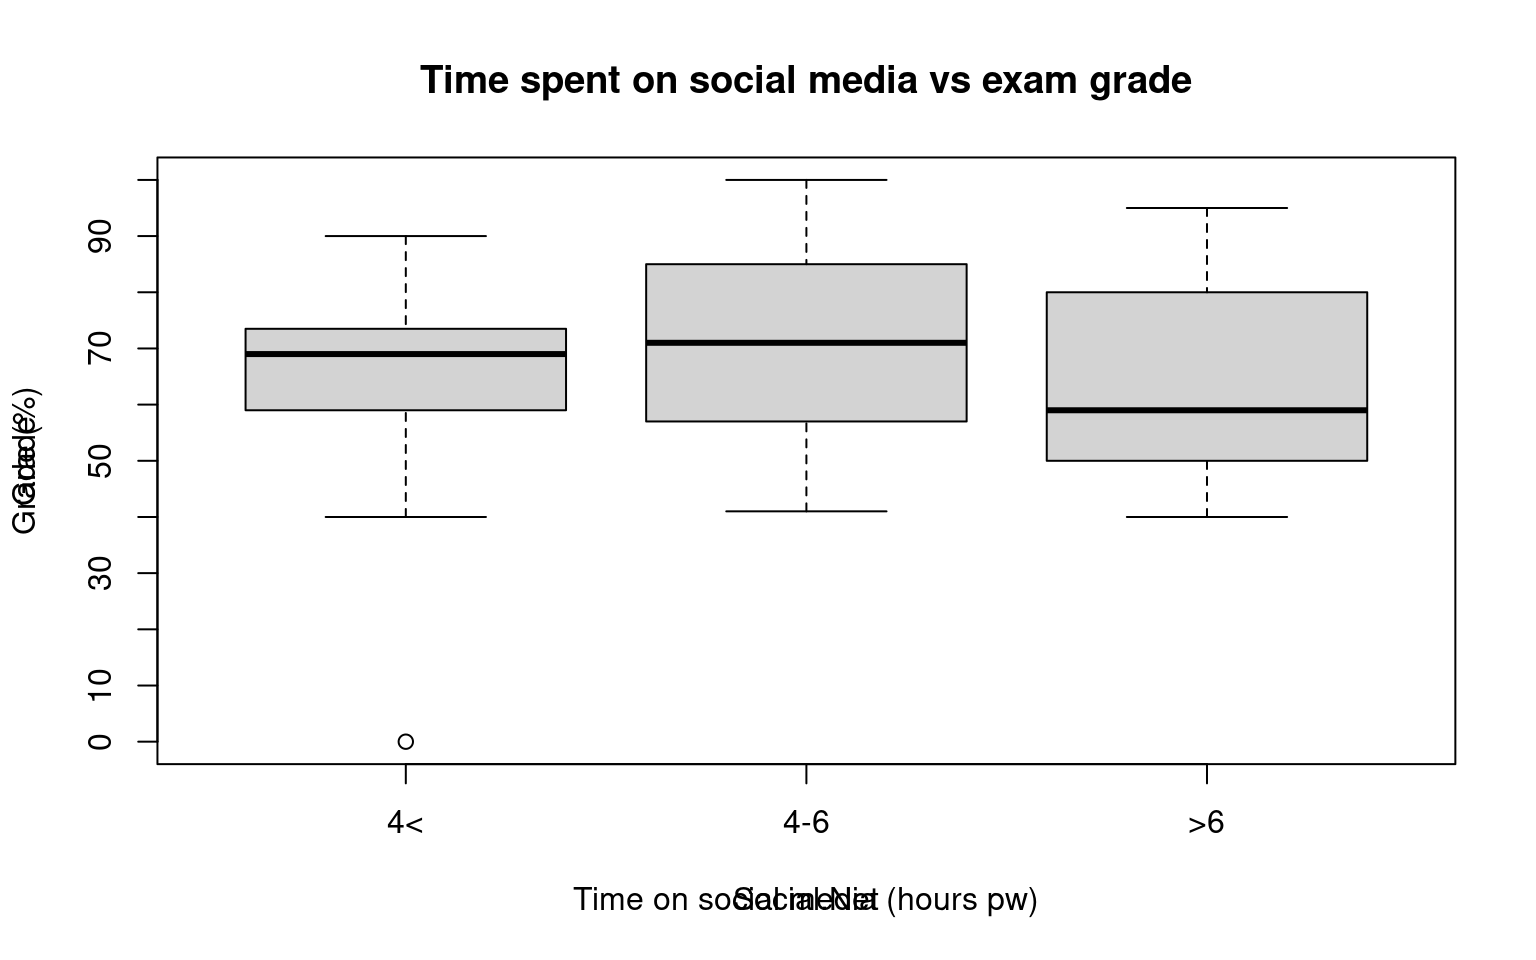
\includegraphics{_main_files/figure-latex/unnamed-chunk-33-1.pdf}

Boxplots can be used to see if there is an association between the outcome and the categorical predictor. We determine this by looking at how different the medians/boxes are from each other.

\fcolorbox{black}{white}{\color{black}
\begin{minipage}[c][6cm][t]{\textwidth}
\sffamily\fboxrule.1em\fboxsep1em
Q: Do you think there is an association between the number of hours spent on social media and exam grades? 
\end{minipage}}

\newpage

\hypertarget{q-q-plots}{%
\subsection{Q-Q plots}\label{q-q-plots}}

Q-Q plots are quantile-quantile plots and are closely related to P-P plots (probability plots). We use them in residual analysis in Regression. A Q-Q plot has the quantiles of the standard normal distribution on the x-axis and plots them against the \emph{observed quantiles} (i.e.~the quantiles corresponding to the observed histogram) of the data (in our usage the standardised residuals).

\color{white} zzzzzz \color{black} \fcolorbox{black}{lightgray!20!white}{\color{black}
\begin{minipage}[c][3.5cm][t]{12.5cm}
\textbf{What is a quantile?} They are points that divide the sample into sections that contain equal probabilities. The median is the central quantile so that half the points in the sample are above it and half the points are below it. The quartiles -- 25th, 50th (median) and 75th-- divide the sample into 4 sections so that a quarter of the points are below the 25th, half are below the 50th and 3/4 are below the 75th. Wikipedia have a good example on how to determine quartiles (or indeed other quantiles) in their entry on quantiles. For the Q-Q plot n-tiles are created where n is the sample size\\
\end{minipage}}

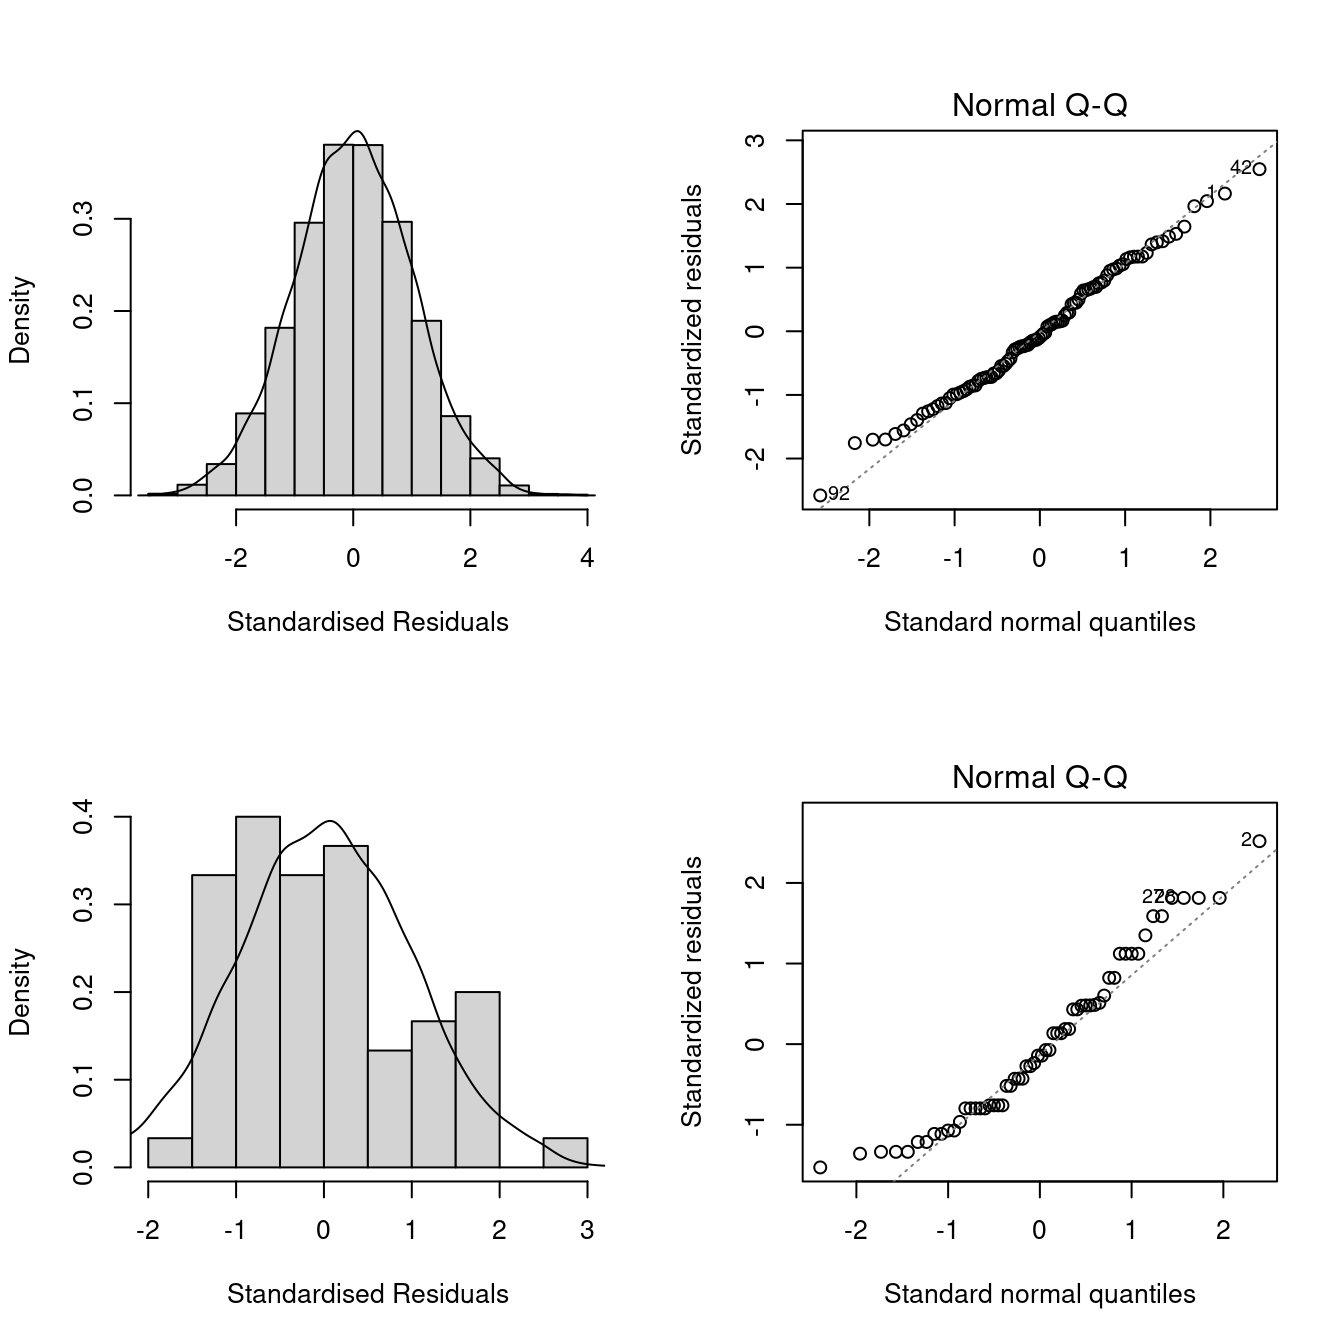
\includegraphics{_main_files/figure-latex/unnamed-chunk-34-1.pdf}

\begin{itemize}
\tightlist
\item
  The top LHS is the histogram of points drawn from a standard normal distribution (N(0,1)) with the standard normal density overlayed. We can see that the histogram is perfectly represented by the density plot.
\item
  The top RHS plot is the corresponding Q-Q plot. It plots the standard normal quantiles against the quantiles of the points from the standard normal (the same ones as in the LHS plot). The dotted line is the x=y diagonal. We can see that the standard normal quantiles and those associated with the sample from the normal are mostly on the x=y diagonal (although sometimes there are some outliers)
\item
  The Q-Q plot assesses how close to normal the standardised residuals are.
\item
  The bottom plots show the standardised residuals from one of our regressions later in the course (I will explain). We can see from both the histogram and the Q-Q plot that these values are not very close to the normal distribution.
\end{itemize}

As we can see from the plots the histogram has more observations in the low quantiles which corresponds to the larger than standard normal quantile values in the y-axis of the Q-Q plot.

\fcolorbox{black}{white}{\color{black}
\begin{minipage}[c][10cm][t]{\textwidth}
\sffamily\fboxrule.1em\fboxsep1em
Q: Can you spot any more features in the two top plots that correspond to one another?
\end{minipage}}

\hypertarget{workshop-2-manipulating-data-with-r}{%
\section{\texorpdfstring{Workshop 2: Manipulating data with \texttt{R}}{Workshop 2: Manipulating data with R}}\label{workshop-2-manipulating-data-with-r}}

\hypertarget{learning-outcomes-2}{%
\subsection{Learning Outcomes}\label{learning-outcomes-2}}

To learn how to load, check correctness of and manipulate data sets in \texttt{R}.

\hypertarget{preamble}{%
\subsection{Preamble}\label{preamble}}

\begin{itemize}
\tightlist
\item
  Create a new folder (Week 2)
\item
  Open \texttt{RStudio}
\item
  Download the data (on the Moodle page for Week 2) into the folder
\item
  Check it's the right folder (\texttt{dir()} lists what is in it)
\item
  If not:

  \begin{itemize}
  \tightlist
  \item
    Go to the Files tab in the bottom right hand corner of \texttt{RStudio}
  \item
    Navigate to the File where you saved the data (e.g.~ST211Week2)
  \item
    Click on More at the top of the tab
  \item
    Select ``Set as Working Directory'' from the drop-down menu
  \end{itemize}
\end{itemize}

\hypertarget{r-packages}{%
\subsection{\texorpdfstring{\texttt{R} packages}{R packages}}\label{r-packages}}

\begin{itemize}
\tightlist
\item
  Packages are libraries of functions in \texttt{R} code that someone else has designed and coded.
\item
  In this course we'll use ``arm'',``ggplot2'' and some others
\item
  Today I need you to install \texttt{arm}, \texttt{ggplot2} and \texttt{gridExtra}
\end{itemize}

\hypertarget{installing-r-packages}{%
\subsection{\texorpdfstring{Installing \texttt{R} packages}{Installing R packages}}\label{installing-r-packages}}

For your laptops you need to install the packages first:

\begin{itemize}
\tightlist
\item
  Go to Packages in the bottom right hand corner of \texttt{RStudio}
\item
  Click on Install
\item
  Type arm/ggplot2/gridExtra and then click on Install
\item
  Some code will run and arm will appear on the list of User library
\end{itemize}

\hypertarget{loading-r-packages}{%
\subsection{\texorpdfstring{Loading \texttt{R} packages}{Loading R packages}}\label{loading-r-packages}}

To use \texttt{R} packages you can either:

Type this in the command line (this is useful to do when you are saving code in a script so that you don't need to manually load packages before running it)

\begin{Shaded}
\begin{Highlighting}[]
\FunctionTok{library}\NormalTok{(arm)}
\end{Highlighting}
\end{Shaded}

Or via the \texttt{Packages} tab in the bottom right hand corner of \texttt{RStudio}. From this tab select the ``arm'' package from the list of available packages

\hypertarget{the-arm-package}{%
\subsection{The ``arm'' package}\label{the-arm-package}}

The main advantage of ``arm'' is that is allows us to use the \texttt{display()} function with linear models. This has less output than the standard \texttt{summary()} command.

\textbf{If you cannot load ``arm''} then you can use \texttt{summary()} instead of \texttt{display()}.

\hypertarget{reading-data-into-r}{%
\subsection{\texorpdfstring{Reading data into \texttt{R}}{Reading data into R}}\label{reading-data-into-r}}

Data is essential for analysis so learning to load it into \texttt{R} is very important. We load two types of data files into \texttt{R}:

\begin{itemize}
\tightlist
\item
  \texttt{.csv} -- When a file is a \texttt{.csv} file we load it using \texttt{read.csv()}.
\item
  \texttt{.txt} -- For \texttt{.txt} file we use \texttt{read.table()}.
\end{itemize}

\texttt{R} can handle many more (e.g.~\texttt{.csv}, STATA and SAS files) with special packages as well.

\begin{itemize}
\tightlist
\item
  Load a file of \texttt{age} in years by \texttt{gender} (male is 1 and female is 0) and hourly pay (\texttt{hourpay}) in £ taken from the British Household Panel Survey.
\item
  The file is in Moodle.
\item
  \emph{Make sure you download it and save it into your working directory before you try and open it}.
\end{itemize}

\begin{Shaded}
\begin{Highlighting}[]
\NormalTok{first.dat}\OtherTok{\textless{}{-}}\FunctionTok{read.csv}\NormalTok{(}\StringTok{"../Data/age\_hourpay.csv"}\NormalTok{,}\AttributeTok{header =} \ConstantTok{TRUE}\NormalTok{)}
\NormalTok{wrong.dat}\OtherTok{\textless{}{-}}\FunctionTok{read.table}\NormalTok{(}\StringTok{"../Data/age\_hourpay.csv"}\NormalTok{,}\AttributeTok{header=}\ConstantTok{TRUE}\NormalTok{)}
\end{Highlighting}
\end{Shaded}

\begin{itemize}
\tightlist
\item
  Loading data with the wrong command will result in a nonsense file although not always with an error.
\item
  You can always look at the Environment tab (top left hand corner of \texttt{RStudio}) to make sure.
\item
  If the length is 1 or there is only 1 variable it is probably wrong.
\end{itemize}

\small

\begin{itemize}
\tightlist
\item
  The name of the file ``age\_hourpay.csv'' must be in ``\,``.
\item
  This is the \emph{path} that \texttt{R} must take to get to the data file.
\item
  If the file is not in the folder \texttt{RStudio} is running from then you will have to change the path accordingly. (Check using \texttt{dir()} )
\item
  \texttt{header=TRUE} tells \texttt{R} that the first line of the data should be taken as the \emph{names} of the columns and thus variables in the loaded file.
\item
  Open your \texttt{.csv} file using Excel and you'll see what I mean.
\item
  When \texttt{R} reads a data file using \texttt{read.csv} or \texttt{read.table} (provided the correct function is used to read it) it creates a \texttt{data.frame}.
\item
  This is the type of data object we will be working with the most and today we will learn to manipulate it.
\item
  We read the data frame into an object(variable) rather than just writing\\
  - \texttt{read.csv("age\_hourpay.csv",header\ =\ TRUE)} because often our data files are large and then the whole console is taken over by showing the data.
\item
  To see the data, go to the Environment tab in the top left hand corner and click on the grid shape at the end of the line corresponding to the data. The data will appear over the console.
\end{itemize}

\hypertarget{accessing-elements-of-the-data-frame}{%
\subsection{Accessing elements of the data frame}\label{accessing-elements-of-the-data-frame}}

Many of the commands and functions for arrays/vectors work for data frames too. For example:

\begin{Shaded}
\begin{Highlighting}[]
\FunctionTok{dim}\NormalTok{(first.dat)}
\end{Highlighting}
\end{Shaded}

\begin{verbatim}
## [1] 10458     3
\end{verbatim}

\begin{Shaded}
\begin{Highlighting}[]
\NormalTok{first.dat[}\DecValTok{55}\NormalTok{,}\DecValTok{2}\NormalTok{]}
\end{Highlighting}
\end{Shaded}

\begin{verbatim}
## [1] 56
\end{verbatim}

\fcolorbox{black}{white}{\color{black}
\begin{minipage}[c][1.5cm][t]{\textwidth}
\sffamily\fboxrule.1em\fboxsep1em
Q: What is code to obtain the the age of the 934th individual in the data frame? Bear in mind that age is in the 2nd column. 
\end{minipage}}

\hypertarget{some-functions-for-data-frames}{%
\subsection{\texorpdfstring{Some \emph{functions} for data frames}{Some functions for data frames}}\label{some-functions-for-data-frames}}

\footnotesize

\begin{Shaded}
\begin{Highlighting}[]
\FunctionTok{colnames}\NormalTok{(first.dat)}
\end{Highlighting}
\end{Shaded}

\begin{verbatim}
## [1] "gender"  "age"     "hourpay"
\end{verbatim}

\begin{Shaded}
\begin{Highlighting}[]
\FunctionTok{head}\NormalTok{(first.dat)}
\end{Highlighting}
\end{Shaded}

\begin{verbatim}
##   gender age hourpay
## 1      0  56  932.50
## 2      0  51  320.51
## 3      0  39  265.40
## 4      0  46  259.28
## 5      0  47  201.93
## 6      0  60  144.25
\end{verbatim}

\begin{Shaded}
\begin{Highlighting}[]
\FunctionTok{head}\NormalTok{(wrong.dat)}
\end{Highlighting}
\end{Shaded}

\begin{verbatim}
##   gender.age.hourpay
## 1         0,56,932.5
## 2        0,51,320.51
## 3         0,39,265.4
## 4        0,46,259.28
## 5        0,47,201.93
## 6        0,60,144.25
\end{verbatim}

\footnotesize

\begin{Shaded}
\begin{Highlighting}[]
\FunctionTok{tail}\NormalTok{(first.dat)}
\end{Highlighting}
\end{Shaded}

\begin{verbatim}
##       gender age hourpay
## 10453      1  39    0.78
## 10454      1  50    0.73
## 10455      0  22    0.60
## 10456      0  29    0.60
## 10457      1  27    0.57
## 10458      1  46    0.47
\end{verbatim}

\begin{itemize}
\tightlist
\item
  \texttt{head()} allows you to look at the first 6 rows of the data
\item
  Whenever calling a large data set (even a large subset of data) it is useful to look at \texttt{head()} only as otherwise the data will fill all the console.
\end{itemize}

\begin{Shaded}
\begin{Highlighting}[]
\FunctionTok{head}\NormalTok{(first.dat, }\DecValTok{3}\NormalTok{)}
\end{Highlighting}
\end{Shaded}

\begin{verbatim}
##   gender age hourpay
## 1      0  56  932.50
## 2      0  51  320.51
## 3      0  39  265.40
\end{verbatim}

\footnotesize

\texttt{summary()} gives a summary of the data columns.

\begin{Shaded}
\begin{Highlighting}[]
\FunctionTok{summary}\NormalTok{(first.dat)}
\end{Highlighting}
\end{Shaded}

\begin{verbatim}
##      gender            age          hourpay       
##  Min.   :0.0000   Min.   :16.0   Min.   :  0.470  
##  1st Qu.:0.0000   1st Qu.:32.0   1st Qu.:  7.543  
##  Median :1.0000   Median :42.0   Median : 10.845  
##  Mean   :0.5291   Mean   :41.5   Mean   : 13.525  
##  3rd Qu.:1.0000   3rd Qu.:51.0   3rd Qu.: 16.490  
##  Max.   :1.0000   Max.   :65.0   Max.   :932.500
\end{verbatim}

You'll see that the \texttt{summary()} function is versatile and can be applied to many \texttt{R} objects.

\hypertarget{setting-conditions}{%
\subsection{Setting conditions}\label{setting-conditions}}

Let's say we are interested in knowing whether there are people in this data that are below 18.

\begin{enumerate}
\def\labelenumi{\arabic{enumi}.}
\tightlist
\item
  First specify which data set
\item
  Then specify which variable using the \texttt{\$} symbol
\end{enumerate}

\begin{Shaded}
\begin{Highlighting}[]
\NormalTok{first.dat}\SpecialCharTok{$}\NormalTok{age}
\end{Highlighting}
\end{Shaded}

\begin{itemize}
\tightlist
\item
  The \texttt{\$} symbol says -- go into \texttt{first.dat} and take only the column named \texttt{age}.
\item
  This is a simple but clunky way of accessing the individual columns (variables) in the data.
\item
  It can also be dangerous as \texttt{RStudio} sometimes auto-completes so if you have two variables named ``age'' and ``agent'' you may, without realising, end up with very different results.
\end{itemize}

We could also have written:

\begin{Shaded}
\begin{Highlighting}[]
\NormalTok{first.dat[,}\DecValTok{2}\NormalTok{]}
\end{Highlighting}
\end{Shaded}

To use this however, you have to know which column corresponds to which variable.

As you can see we've produced lots of data and have maxed out the console. Always use \texttt{head()}:

\begin{Shaded}
\begin{Highlighting}[]
\FunctionTok{head}\NormalTok{(first.dat[,}\DecValTok{2}\NormalTok{])}
\end{Highlighting}
\end{Shaded}

\begin{verbatim}
## [1] 56 51 39 46 47 60
\end{verbatim}

\begin{enumerate}
\def\labelenumi{\arabic{enumi}.}
\setcounter{enumi}{2}
\tightlist
\item
  Now set your condition \textless{} 18.
\end{enumerate}

Start by trying this:

\begin{Shaded}
\begin{Highlighting}[]
\FunctionTok{head}\NormalTok{(first.dat}\SpecialCharTok{$}\NormalTok{age}\SpecialCharTok{\textless{}}\DecValTok{18}\NormalTok{)}
\end{Highlighting}
\end{Shaded}

\begin{verbatim}
## [1] FALSE FALSE FALSE FALSE FALSE FALSE
\end{verbatim}

\begin{itemize}
\tightlist
\item
  It is not ideal because it goes through first.dat{[},2{]} row by row and answers the question ``is this number under 18?''.
\item
  If it is not not the command assigns \texttt{FALSE} otherwise \texttt{TRUE}.
\item
  We usually want to know \emph{which} elements satisfy the condition, i.e.~we want a list of positions in the data frame of the elements where the age\textless18.
\end{itemize}

\begin{enumerate}
\def\labelenumi{\arabic{enumi}.}
\setcounter{enumi}{3}
\tightlist
\item
  So which are they?
\end{enumerate}

\begin{Shaded}
\begin{Highlighting}[]
\FunctionTok{which}\NormalTok{(first.dat}\SpecialCharTok{$}\NormalTok{age}\SpecialCharTok{\textless{}}\DecValTok{18}\NormalTok{)}
\end{Highlighting}
\end{Shaded}

\begin{itemize}
\tightlist
\item
  This gives their row number in first.dat.
\item
  We can use this list to see how many there are, create a new data set, look at the values of gender for these, etc.
\end{itemize}

\begin{enumerate}
\def\labelenumi{\arabic{enumi}.}
\setcounter{enumi}{4}
\tightlist
\item
  How many are they?
\end{enumerate}

\begin{Shaded}
\begin{Highlighting}[]
\FunctionTok{length}\NormalTok{(}\FunctionTok{which}\NormalTok{(first.dat}\SpecialCharTok{$}\NormalTok{age}\SpecialCharTok{\textless{}}\DecValTok{18}\NormalTok{))}
\end{Highlighting}
\end{Shaded}

\begin{verbatim}
## [1] 141
\end{verbatim}

\begin{enumerate}
\def\labelenumi{\arabic{enumi}.}
\setcounter{enumi}{5}
\tightlist
\item
  Let's create a new data.frame with just these people and find out how many women and men there are.
\end{enumerate}

\begin{Shaded}
\begin{Highlighting}[]
\NormalTok{under18}\OtherTok{\textless{}{-}}\NormalTok{first.dat[}\FunctionTok{which}\NormalTok{(first.dat}\SpecialCharTok{$}\NormalTok{age}\SpecialCharTok{\textless{}}\DecValTok{18}\NormalTok{),]}
\FunctionTok{table}\NormalTok{(under18}\SpecialCharTok{$}\NormalTok{gender)}
\end{Highlighting}
\end{Shaded}

\begin{verbatim}
## 
##  0  1 
## 57 84
\end{verbatim}

Say we want to ignore those below 18 years of age in our analysis. How do we do this? Here are three equivalent expressions

\begin{Shaded}
\begin{Highlighting}[]
\NormalTok{over18}\OtherTok{\textless{}{-}}\NormalTok{first.dat[}\FunctionTok{which}\NormalTok{(first.dat}\SpecialCharTok{$}\NormalTok{age}\SpecialCharTok{\textgreater{}=}\DecValTok{18}\NormalTok{),]}
\FunctionTok{dim}\NormalTok{(over18)}
\end{Highlighting}
\end{Shaded}

\begin{verbatim}
## [1] 10317     3
\end{verbatim}

\begin{Shaded}
\begin{Highlighting}[]
\NormalTok{over18}\OtherTok{\textless{}{-}}\NormalTok{first.dat[first.dat}\SpecialCharTok{$}\NormalTok{age}\SpecialCharTok{\textgreater{}=}\DecValTok{18}\NormalTok{,]}
\FunctionTok{dim}\NormalTok{(over18)}
\end{Highlighting}
\end{Shaded}

\begin{verbatim}
## [1] 10317     3
\end{verbatim}

\begin{Shaded}
\begin{Highlighting}[]
\NormalTok{over18}\OtherTok{\textless{}{-}}\FunctionTok{subset}\NormalTok{(first.dat, age}\SpecialCharTok{\textgreater{}=}\DecValTok{18}\NormalTok{)}
\FunctionTok{dim}\NormalTok{(over18)}
\end{Highlighting}
\end{Shaded}

\begin{verbatim}
## [1] 10317     3
\end{verbatim}

\begin{itemize}
\item
  You can see that first.dat.over18 now has appeared in Environment.
\item
  The simplest and most intuitive is the last command using \texttt{subset()}.
\item
  This function takes a subset of the data (the first argument) with criterion the second argument.
\item
  In this case it takes first.dat and extracts the points where the age is greater or equal to 18.
\item
  I prefer it to the other expressions as it doesn't have the \texttt{\$}, the \texttt{{[}{]}} or the \texttt{which()} .
\end{itemize}

\texttt{subset()} can take multiple conditions:

\begin{Shaded}
\begin{Highlighting}[]
\NormalTok{second.dat}\OtherTok{\textless{}{-}}\FunctionTok{subset}\NormalTok{(first.dat, (age}\SpecialCharTok{\textgreater{}=}\DecValTok{18} \SpecialCharTok{\&}\NormalTok{ hourpay}\SpecialCharTok{\textless{}=}\DecValTok{50}\NormalTok{))}
\end{Highlighting}
\end{Shaded}

\begin{itemize}
\tightlist
\item
  To do regression we need to use data.
\item
  We've see how to load data into \texttt{R} and how do do some manipulations (e.g.~\texttt{subset()}) and queries (e.g.~\texttt{which()}).
\item
  We've seen how to use the \texttt{\$} sign to access variables inside data sets, however if we are doing multiple things (such as the previous command) it starts getting really ugly.
\end{itemize}

\texttt{with()} makes things simple and has the same syntax as \texttt{subset()}. It takes two arguments.

\begin{itemize}
\tightlist
\item
  the name of the data set in \texttt{R}
\item
  the function or operation you want to do to variables in the data.
\end{itemize}

\begin{Shaded}
\begin{Highlighting}[]
\FunctionTok{with}\NormalTok{(first.dat, }\FunctionTok{mean}\NormalTok{(gender}\SpecialCharTok{==}\DecValTok{0}\NormalTok{))}
\end{Highlighting}
\end{Shaded}

\begin{verbatim}
## [1] 0.4709313
\end{verbatim}

\hypertarget{scatter-plots}{%
\subsection{Scatter plots}\label{scatter-plots}}

\begin{itemize}
\tightlist
\item
  One of the first things you should do with a new dataset is plot the data in whatever way is possible.
\item
  For continuous variables a scatter plot is usually used.
\item
  \texttt{plot()} is a very flexible function and traditionally did a lot of the plotting in \texttt{R}.
\end{itemize}

We'll plot age on the x-axis and log(hourpay) on the y-axis. Try plotting age against hourpay to see why we use logs

\begin{Shaded}
\begin{Highlighting}[]
\FunctionTok{with}\NormalTok{(over18, }\FunctionTok{plot}\NormalTok{(age,hourpay))}
\end{Highlighting}
\end{Shaded}

\begin{Shaded}
\begin{Highlighting}[]
\FunctionTok{with}\NormalTok{(over18, }\FunctionTok{plot}\NormalTok{(age,}\FunctionTok{log}\NormalTok{(hourpay)))}
\end{Highlighting}
\end{Shaded}

\hypertarget{ggplot2-package}{%
\subsection{\texorpdfstring{\texttt{ggplot2} package}{ggplot2 package}}\label{ggplot2-package}}

\begin{itemize}
\tightlist
\item
  For better and more complex plots
\item
  We will be using this most of the time.
\item
  At the end of your book is a dedicated section on how to use this package with step-by-step instructions.
\item
  \emph{Spend some time going over this as we will be using it a lot.}
\item
  Install \texttt{ggplot2} and \texttt{gridExtra}
\end{itemize}

\begin{Shaded}
\begin{Highlighting}[]
\FunctionTok{library}\NormalTok{(ggplot2)}
\FunctionTok{library}\NormalTok{(gridExtra)}
\end{Highlighting}
\end{Shaded}

\footnotesize

\begin{Shaded}
\begin{Highlighting}[]
\NormalTok{p1}\OtherTok{\textless{}{-}}\FunctionTok{ggplot}\NormalTok{(over18, }\FunctionTok{aes}\NormalTok{(}\AttributeTok{x=}\NormalTok{age, }\AttributeTok{y=}\FunctionTok{log}\NormalTok{(hourpay),}\AttributeTok{colour=}\FunctionTok{factor}\NormalTok{(gender)))}
\NormalTok{p1}\OtherTok{\textless{}{-}}\NormalTok{ p1 }\SpecialCharTok{+} \FunctionTok{geom\_point}\NormalTok{(}\AttributeTok{size=}\FloatTok{0.5}\NormalTok{,}\FunctionTok{aes}\NormalTok{(}\AttributeTok{colour=}\FunctionTok{factor}\NormalTok{(gender)))}
\NormalTok{p1}\OtherTok{\textless{}{-}}\NormalTok{ p1 }\SpecialCharTok{+}\FunctionTok{scale\_colour\_grey}\NormalTok{(}\AttributeTok{start =} \FloatTok{0.1}\NormalTok{, }\AttributeTok{end =} \FloatTok{0.6}\NormalTok{)  }\SpecialCharTok{+} \FunctionTok{theme\_bw}\NormalTok{()}
\NormalTok{p1}\OtherTok{\textless{}{-}}\NormalTok{ p1}\SpecialCharTok{+} \FunctionTok{theme}\NormalTok{(}\AttributeTok{legend.position =} \FunctionTok{c}\NormalTok{(}\FloatTok{0.35}\NormalTok{,}\FloatTok{0.9}\NormalTok{), }
               \AttributeTok{legend.direction =} \StringTok{"horizontal"}\NormalTok{)}
\NormalTok{p1}\OtherTok{\textless{}{-}}\NormalTok{ p1}\SpecialCharTok{+} \FunctionTok{ggtitle}\NormalTok{(}\StringTok{"log(Hourly pay) by age and gender"}\NormalTok{)}
\NormalTok{p1 }\OtherTok{\textless{}{-}}\NormalTok{ p1}\SpecialCharTok{+} \FunctionTok{geom\_smooth}\NormalTok{(}\AttributeTok{method=}\StringTok{"lm"}\NormalTok{,}\AttributeTok{fill=}\ConstantTok{NA}\NormalTok{)}


\NormalTok{p2}\OtherTok{\textless{}{-}}\FunctionTok{ggplot}\NormalTok{(over18, }\FunctionTok{aes}\NormalTok{(}\AttributeTok{x=}\NormalTok{age, }\AttributeTok{y=}\FunctionTok{log}\NormalTok{(hourpay))) }
\NormalTok{p2}\OtherTok{\textless{}{-}}\NormalTok{ p2 }\SpecialCharTok{+} \FunctionTok{geom\_jitter}\NormalTok{(}\AttributeTok{size=}\FloatTok{0.5}\NormalTok{,}\FunctionTok{aes}\NormalTok{(}\AttributeTok{colour=}\FunctionTok{factor}\NormalTok{(gender))) }
\NormalTok{p2}\OtherTok{\textless{}{-}}\NormalTok{  p2 }\SpecialCharTok{+} \FunctionTok{scale\_colour\_grey}\NormalTok{(}\AttributeTok{start =} \FloatTok{0.1}\NormalTok{, }\AttributeTok{end =}\NormalTok{ .}\DecValTok{6}\NormalTok{)  }\SpecialCharTok{+} \FunctionTok{theme\_bw}\NormalTok{()}
\NormalTok{p2}\OtherTok{\textless{}{-}}\NormalTok{ p2}\SpecialCharTok{+} \FunctionTok{theme}\NormalTok{(}\AttributeTok{legend.position =} \StringTok{"none"}\NormalTok{)}
\NormalTok{p2}\OtherTok{\textless{}{-}}\NormalTok{ p2}\SpecialCharTok{+} \FunctionTok{ggtitle}\NormalTok{(}\StringTok{"log(Hourly pay) by age and gender"}\NormalTok{)}
\end{Highlighting}
\end{Shaded}

\begin{Shaded}
\begin{Highlighting}[]
\FunctionTok{grid.arrange}\NormalTok{(p1,p2,}\AttributeTok{ncol=}\DecValTok{2}\NormalTok{)}
\end{Highlighting}
\end{Shaded}

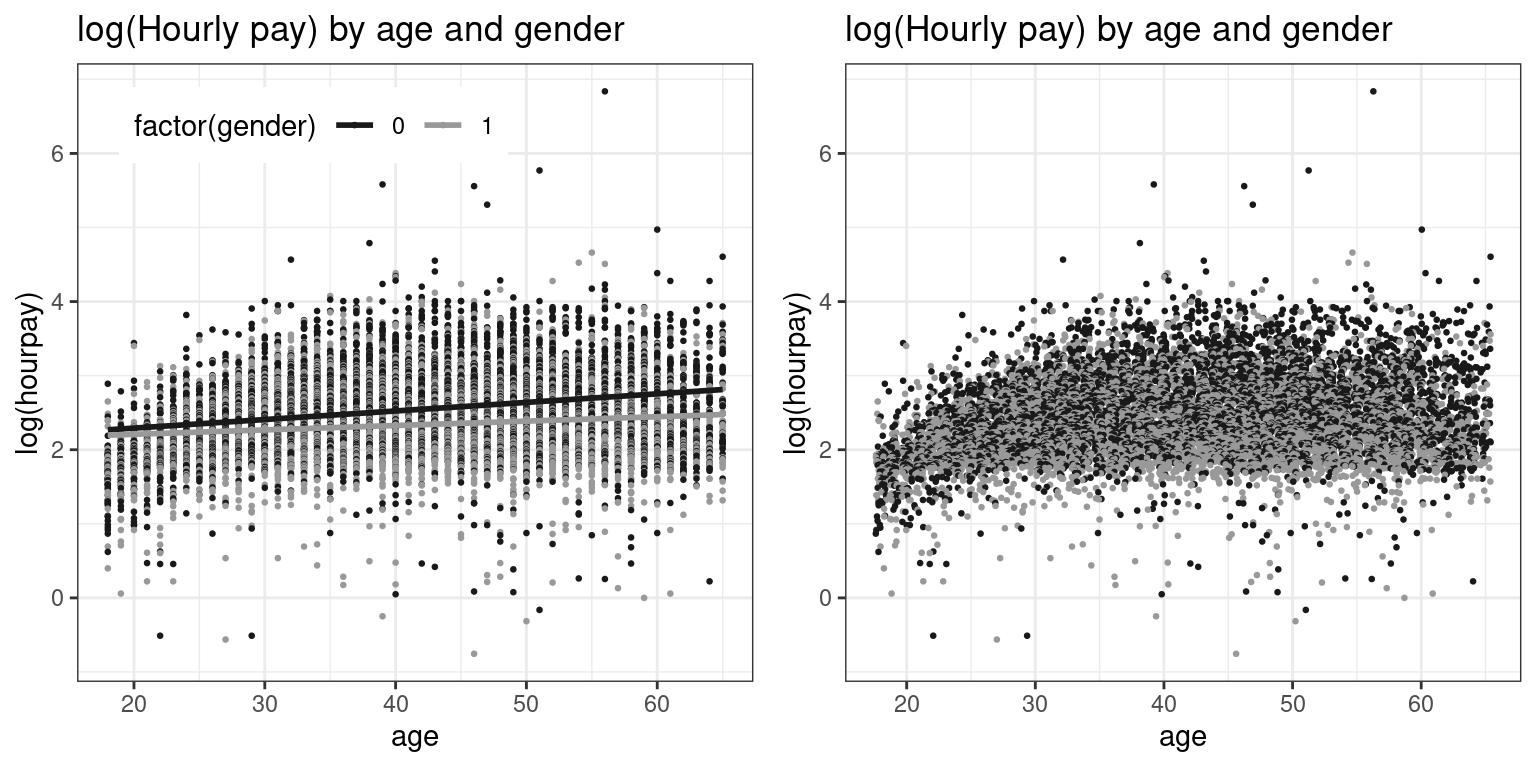
\includegraphics{_main_files/figure-latex/unnamed-chunk-55-1.pdf}

\hypertarget{saving-data}{%
\subsection{Saving data}\label{saving-data}}

\begin{itemize}
\tightlist
\item
  It is often the case that we want to change an existing data set or create a new one.
\item
  In these situations we need to be able to save the data. For example we created the \texttt{over18} data from the \texttt{first.dat}.
\item
  Rather than have to re-create it every time we want to use it, we may find it easier to save it directly.
\item
  There are a number of ways but the one I prefer is using \texttt{write.csv}.
\end{itemize}

\begin{Shaded}
\begin{Highlighting}[]
\FunctionTok{write.csv}\NormalTok{(over18, }\StringTok{"Over18\_age\_hourpay.csv"}\NormalTok{)}
\end{Highlighting}
\end{Shaded}

\begin{itemize}
\tightlist
\item
  If you run this and get no errors then you should check that there is a new .csv file names Over18\_age\_hourpay.csv in your working directory.
\item
  It will also save in the image if you choose to save that
\end{itemize}

The arguments of \texttt{write.csv} are:

\begin{itemize}
\tightlist
\item
  the name of the \texttt{data.frame} to save in \texttt{R}
\item
  the name of the .csv file the \texttt{data.frame} should be saved into -- because it is outside of \texttt{R} it needs to be in ``\,''
\item
  \texttt{row.names=FALSE} is an optional argument. If it is not included in the call to \texttt{write.csv} then it automatically adds a column with the row number to the data. This is very annoying when you later open the dataset and find an additional row.
\end{itemize}

\begin{Shaded}
\begin{Highlighting}[]
\FunctionTok{write.csv}\NormalTok{(over18, }\StringTok{"Over18\_age\_hourpay.csv"}\NormalTok{,}\AttributeTok{row.names=}\ConstantTok{FALSE}\NormalTok{)}
\end{Highlighting}
\end{Shaded}

and see what the .csv file looks like.

\hypertarget{built-in-functions}{%
\subsection{Built in functions}\label{built-in-functions}}

\texttt{R} has a large number of built in functions. We've seen a few already

\begin{itemize}
\item
  \texttt{log()}
\item
  \texttt{plot()}
\item
  \texttt{read.csv()}
\item
  \texttt{subset()}
\item
  \texttt{which()}
\item
  \texttt{length()}
\item
  \texttt{dim()}
\item
  We'll learn many more and also how to write some basic functions.
\item
  Functions work as follows:

  \begin{itemize}
  \tightlist
  \item
    They have a name e.g.~\texttt{plot()}.\\
  \item
    Inside the brackets you enter the \emph{arguments} e.g.~\texttt{x}, \texttt{y}, \texttt{pch}, \texttt{main} etc.\\
  \item
    Some arguments are mandatory (e.g.~\texttt{x} and \texttt{y}) and if you don't enter them or they are not of the right form then \texttt{R} returns an error.\\
  \item
    Others (e.g.~\texttt{main}, \texttt{pch} etc.) are optional and \texttt{R} has some default values.
  \end{itemize}
\end{itemize}

\hypertarget{other-functions-useful-for-stats}{%
\subsection{Other functions useful for stats}\label{other-functions-useful-for-stats}}

\begin{itemize}
\tightlist
\item
  \texttt{sum()}
\item
  \texttt{mean()}
\item
  \texttt{sd()}
\item
  \texttt{summary()}
\item
  \texttt{exp()}
\end{itemize}

Try these with our data set.

\hypertarget{doing-the-same-things-to-each-row-or-column}{%
\subsection{Doing the same things to each row or column}\label{doing-the-same-things-to-each-row-or-column}}

\footnotesize

\begin{Shaded}
\begin{Highlighting}[]
\FunctionTok{summary}\NormalTok{(over18)}
\end{Highlighting}
\end{Shaded}

\begin{verbatim}
##      gender            age           hourpay      
##  Min.   :0.0000   Min.   :18.00   Min.   :  0.47  
##  1st Qu.:0.0000   1st Qu.:32.00   1st Qu.:  7.67  
##  Median :1.0000   Median :42.00   Median : 10.94  
##  Mean   :0.5282   Mean   :41.84   Mean   : 13.64  
##  3rd Qu.:1.0000   3rd Qu.:51.00   3rd Qu.: 16.54  
##  Max.   :1.0000   Max.   :65.00   Max.   :932.50
\end{verbatim}

\begin{Shaded}
\begin{Highlighting}[]
\FunctionTok{colMeans}\NormalTok{(over18)}
\end{Highlighting}
\end{Shaded}

\begin{verbatim}
##     gender        age    hourpay 
##  0.5281574 41.8371620 13.6425007
\end{verbatim}

\begin{Shaded}
\begin{Highlighting}[]
\FunctionTok{head}\NormalTok{(}\FunctionTok{rowSums}\NormalTok{(over18))}
\end{Highlighting}
\end{Shaded}

\begin{verbatim}
##      1      2      3      4      5      6 
## 988.50 371.51 304.40 305.28 248.93 204.25
\end{verbatim}

\begin{itemize}
\tightlist
\item
  More about functions, loops, the \texttt{ifelse()} and \texttt{apply()} functions in an exercise in the back of the course notes.
\end{itemize}

\hypertarget{grouping-dataframes}{%
\subsection{Grouping dataframes}\label{grouping-dataframes}}

\begin{itemize}
\tightlist
\item
  We can use \texttt{subset} to group data.
\item
  We can use \texttt{aggregate} to apply functions to subsets.
\end{itemize}

\begin{Shaded}
\begin{Highlighting}[]
\FunctionTok{aggregate}\NormalTok{(over18[,}\SpecialCharTok{{-}}\DecValTok{1}\NormalTok{],over18[}\DecValTok{1}\NormalTok{],mean)}
\end{Highlighting}
\end{Shaded}

\begin{verbatim}
##   gender      age  hourpay
## 1      0 42.09922 15.52974
## 2      1 41.60305 11.95649
\end{verbatim}

\texttt{aggregate} takes the following arguments

\begin{itemize}
\tightlist
\item
  The data to aggregate: in this case the age and hourpay columns
\item
  The column to aggregate them by: in this case the first column of the data
\item
  The function to apply: in this case the mean
\end{itemize}

As you can see the mean age of women working is lower than that of men but those who do work earn more per hour.

\hypertarget{lecture-3-simple-linear-regression}{%
\section{Lecture 3: Simple linear Regression}\label{lecture-3-simple-linear-regression}}

\hypertarget{learning-outcomes-3}{%
\subsection{Learning Outcomes}\label{learning-outcomes-3}}

To understand the basic concepts necessary for performing simple linear regression such as lines, least squares estimates, coefficients.

Diagnostics Part 1: Significance of regression coefficients, \(R^2\) statistics and residual standard deviation

\hypertarget{why-linear-regression}{%
\subsection{Why linear regression?}\label{why-linear-regression}}

The aim of linear regression is to fit the relationship between a predictor and an outcome as a \emph{straight line} with coefficients obtained using \emph{least squares estmation}. There are a number of advantages to linear regression:

\begin{itemize}
\tightlist
\item
  lines are easy to understand/interpret.
\item
  lines are easy to fit: least squares regression has easy to calculate formulae for the estimates of the intercept and the slope.
\item
  together with assumptions about the normality of \(y\) linear regression can lead to relatively easy checks to ensure that the model is appropriate.
\item
  The theory for Hypothesis tests is straightforward.
\end{itemize}

\textbf{How are lines defined in this context:}

A straight line on a graph with an \(x\) and \(y\) axis is given by \(y = \beta_0+\beta_1 x\).

\begin{itemize}
\tightlist
\item
  The line crosses the \(y\) axis at \(\beta_0\): the value for \(y\) at \(x=0\) is \(\beta_0\). \(\beta_0\) is termed the \emph{intercept}
\item
  The line has a \emph{slope/gradient} of \(\beta_1\): an increase in \(x\) of 1 results in a change of \(\beta_1\) in y
\end{itemize}

\hypertarget{terminology}{%
\subsection{Terminology}\label{terminology}}

We will use the following terminology

\begin{itemize}
\tightlist
\item
  A predictor is usually termed \(x\) (with subscripts if more than one) or given a name e.g.~``age''
\item
  The outcome is typically termed \(y\) or given a name e.g.~``hourpay''
\item
  \(\beta\) is the ``true'' coefficient, \(\sigma\) is the ``true'' standard deviation
\item
  Adding a ``hat'' \(\hat{}\) indicates an \emph{estimate} rather than the true underlying value (e.g.~\(\hat{\beta}\) or \(\hat{y_i}\))
\end{itemize}

\hypertarget{estimation}{%
\subsection{Estimation}\label{estimation}}

Below is a plot of 15 data points which relate the number of hours of independent study per week = x on the x-axis to the average grade (\%) in final exams = y on the y-axis for a subset of LSE students:

\begin{Shaded}
\begin{Highlighting}[]
\NormalTok{lse.dat}\OtherTok{\textless{}{-}}\FunctionTok{read.csv}\NormalTok{(}\StringTok{"lsehwk3.csv"}\NormalTok{)}
\FunctionTok{with}\NormalTok{(lse.dat, }\FunctionTok{plot}\NormalTok{(x,y, }\AttributeTok{xlim=}\FunctionTok{c}\NormalTok{(}\DecValTok{0}\NormalTok{,}\DecValTok{15}\NormalTok{),}\AttributeTok{ylim=}\FunctionTok{c}\NormalTok{(}\DecValTok{0}\NormalTok{,}\DecValTok{80}\NormalTok{)))}
\end{Highlighting}
\end{Shaded}

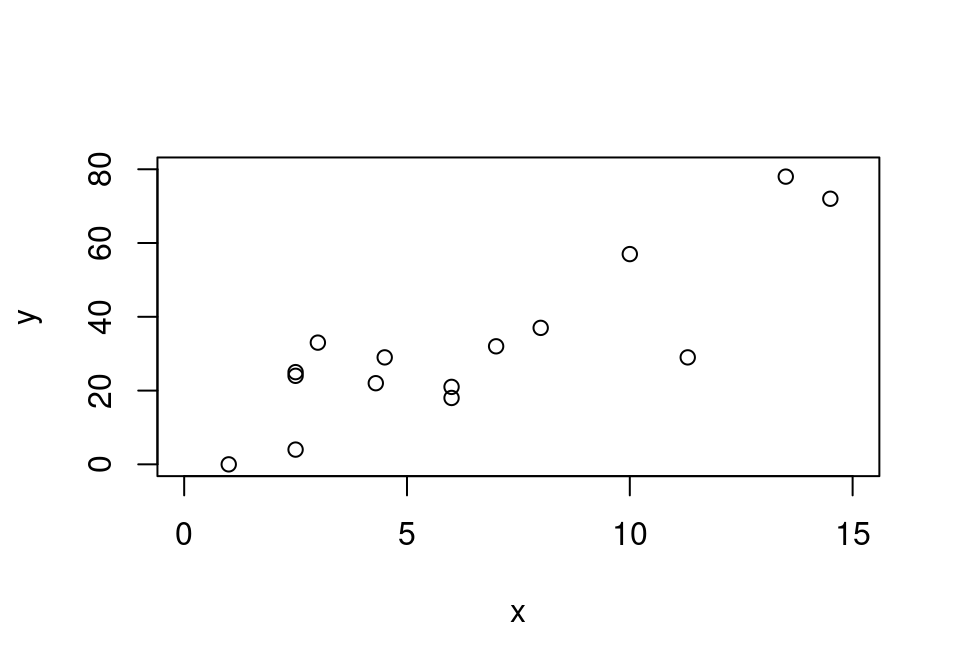
\includegraphics{_main_files/figure-latex/unnamed-chunk-60-1.pdf}

On the plot draw what you think is the line of best fit. Based on this line take a guess at the intercept and the slope. I'm going to guess the intercept it 0 and the slope is 4

\[ \hat{y}_i = 0 + 4 x_i \]

\textbf{``Gue-Estimates''}

My guesses are (crude) \emph{estimates} of the parameters \(\beta_0\) and \(\beta_1\) which we term \(\hat{\beta_0}\) and \(\hat{\beta_1}\). They are estimates rather than the ``true'' parameters because

\begin{enumerate}
\def\labelenumi{\arabic{enumi}.}
\tightlist
\item
  our sample is too small (there are only 15 points)
\item
  we always measure with error (in this case y has been measured using a survey so they are subject to recall bias)
\item
  are there really any true values? The best possible linear model is at most a good approximation
\item
  we are guessing (as opposed to estimating the parameters using techniques which have good mathematical and statistical properties :unbiased, converging to the true value etc.)
\end{enumerate}

\hypertarget{least-squares-estimates}{%
\subsection{Least squares estimates}\label{least-squares-estimates}}

Points 1, 2 and 3 are true for least squares estimates too. However they are not a ``guess'', they are the best estimates possible given the data.
Formally, least squares estimates of the coefficients are those that \emph{minimize} the \emph{sum} of the \emph{squares} of the \emph{observed vertical distance} (termed residual) between the points and the line. We could also minimise the sum of the absolute value of the vertical distances. We prefer the \emph{square} because:

\begin{itemize}
\tightlist
\item
  it has better mathematical properties (it is easy to take a derivative of a square)
\item
  it penalises points that are further away more than an absolute value.
\end{itemize}

In the plot below draw two lines -- one that fits better and another that fits poorly and see how that changes the size of the squares of the vertical distance from the line to the point.

\begin{Shaded}
\begin{Highlighting}[]
\FunctionTok{par}\NormalTok{(}\AttributeTok{mfrow=}\FunctionTok{c}\NormalTok{(}\DecValTok{1}\NormalTok{,}\DecValTok{2}\NormalTok{))}
\NormalTok{lse.dat}\OtherTok{\textless{}{-}}\FunctionTok{read.csv}\NormalTok{(}\StringTok{"lsehwk3.csv"}\NormalTok{)}
\FunctionTok{with}\NormalTok{(lse.dat, }\FunctionTok{plot}\NormalTok{(x,y, }\AttributeTok{xlim=}\FunctionTok{c}\NormalTok{(}\DecValTok{0}\NormalTok{,}\DecValTok{15}\NormalTok{),}\AttributeTok{ylim=}\FunctionTok{c}\NormalTok{(}\DecValTok{0}\NormalTok{,}\DecValTok{80}\NormalTok{)))}
\FunctionTok{with}\NormalTok{(lse.dat, }\FunctionTok{plot}\NormalTok{(x,y, }\AttributeTok{xlim=}\FunctionTok{c}\NormalTok{(}\DecValTok{0}\NormalTok{,}\DecValTok{15}\NormalTok{),}\AttributeTok{ylim=}\FunctionTok{c}\NormalTok{(}\DecValTok{0}\NormalTok{,}\DecValTok{80}\NormalTok{)))}
\end{Highlighting}
\end{Shaded}

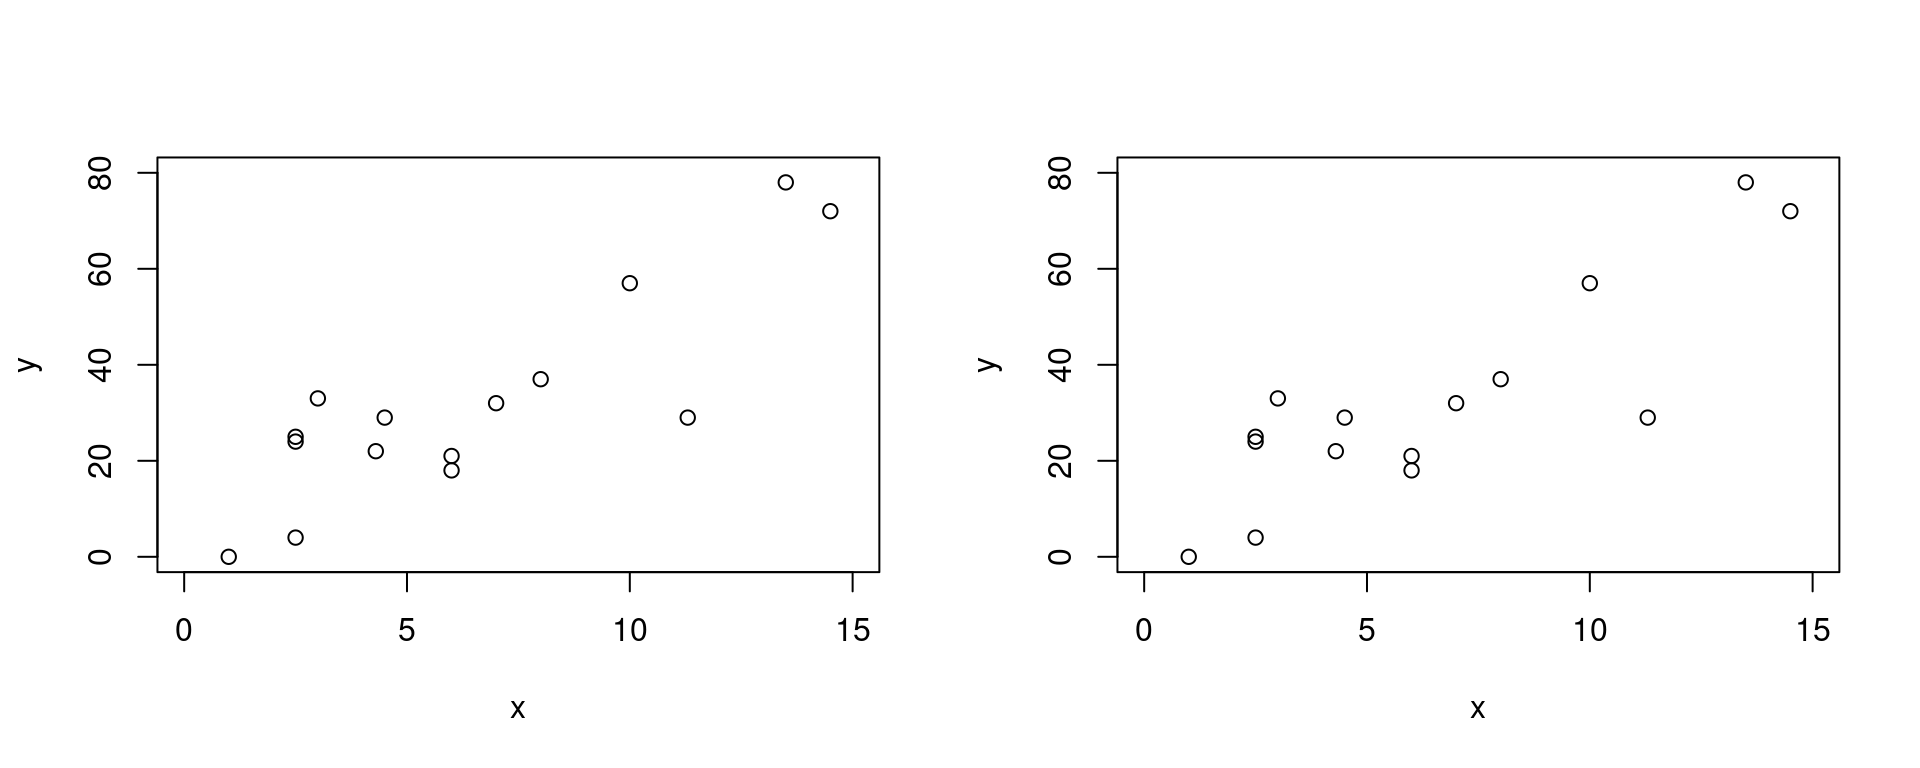
\includegraphics{_main_files/figure-latex/unnamed-chunk-61-1.pdf}

As an aside the least squares line goes through \(\bar{x}\) and \(\bar{y}\) the means(averages) of \(x\) and \(y\) respectively

\hypertarget{the-residuals}{%
\subsection{The residuals}\label{the-residuals}}

The vertical distance between the line of fit and the observed value is called the \emph{residual}. The residuals can be thought of as representing the error in the regression. The bigger they are the worse the fit of the line to the data. Formally:

\[ r_i= y_i - \hat{y_i} = y_i- (\hat{\beta_0}+\hat{\beta_1}x_i) \]

or in the case of our guess:

\[ \begin{aligned}
r_i & = y_i - (\hat{\beta_0}+\hat{\beta_1}y_i)\\  & = y_i - (0 +  4 x_i) 
\end{aligned}
\]

\textbf{Sum of Squares of the error (residuals)}

Formally in least squares estimation the quantity that has to me minimised with respect to the parameters \(\beta_0\) and \(\beta_1\) is:

\[
\begin{aligned}
SSE= &  \sum r_i^2  \\
 =  & \sum [y_i - (\hat{\beta_0}+\hat{\beta_1}x_i)]^2 
\end{aligned}
\]

You will find on Moodle a video with the formal derivation of the least squares estimates using calculus. You \emph{MUST} learn this as something related to this is almost always on the exam.

\newpage

\textbf{Exercise}

Below are 4 very simple plots. Draw the line that you think will be best for predicting \(y\) from \(x\).

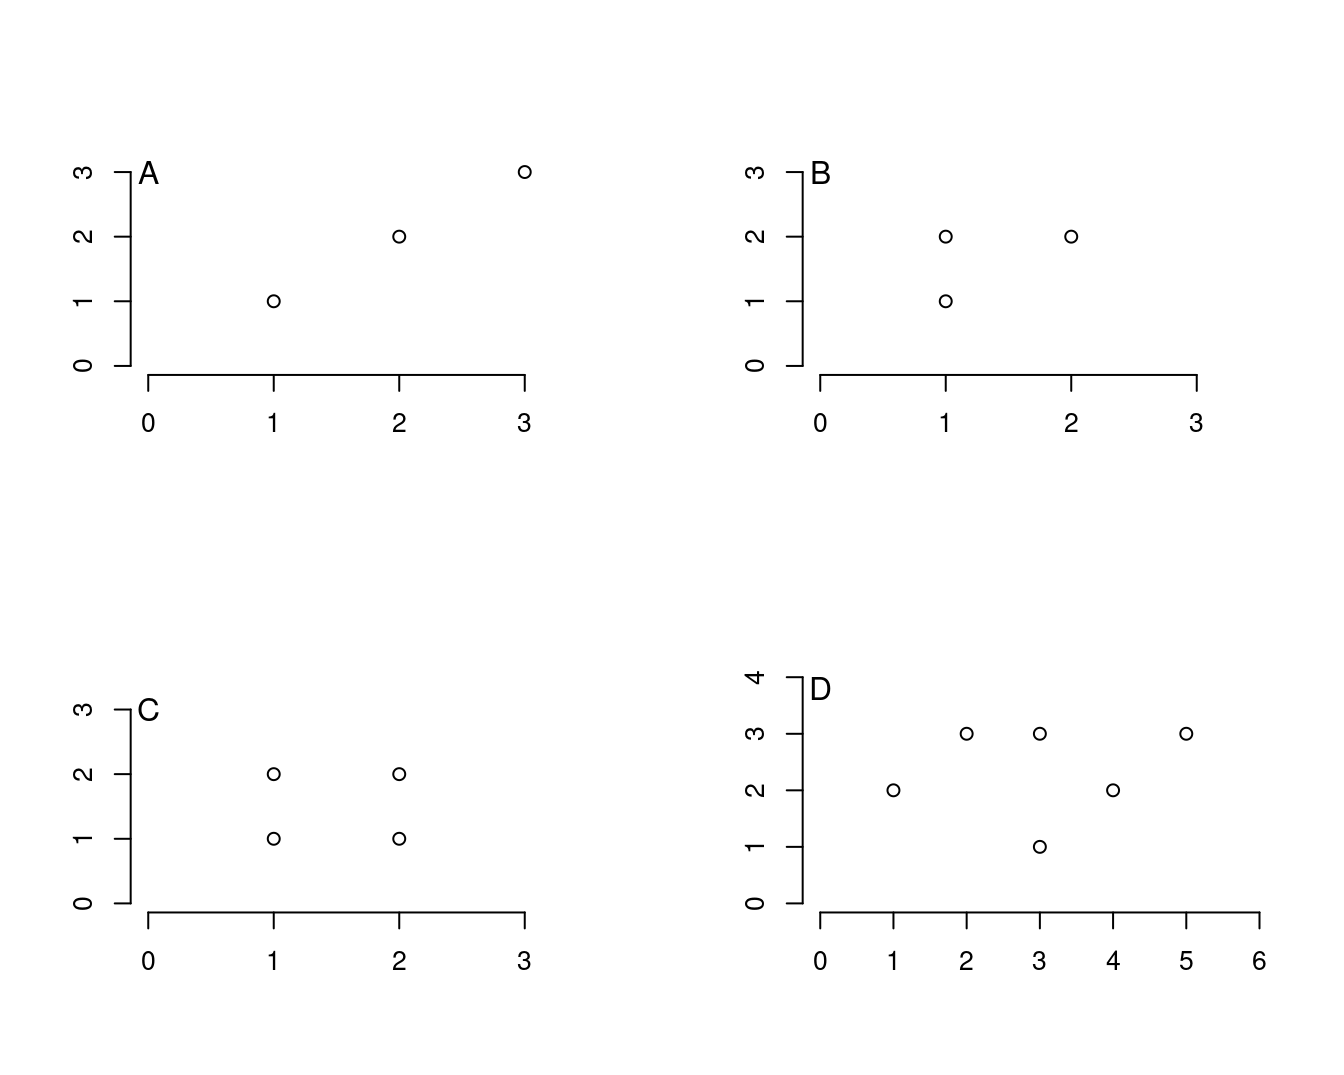
\includegraphics{_main_files/figure-latex/unnamed-chunk-62-1.pdf}
Below are the equations estimated from these data using least squares estimation. Use the four least squares equations to \emph{predict} \(y\) for \(x= \{0,3\}\). Then draw a line through the two points in a different colour: this will be your line of best fit using least squares estimation.

\begin{itemize}
\tightlist
\item
  A: \(y = 0 + x\)
\item
  B: \(y = 1 + 0.5 x\)
\item
  C: \(y = 1.5 + 0 x\)
\item
  D: \(y = 2 + 0.1 x\)
\end{itemize}

\begin{longtable}[]{@{}lllll@{}}
\toprule()
x & A & B & C & D \\
\midrule()
\endhead
0 & & & & \\
--- & --- & --- & --- & --- \\
3 & & & & \\
\bottomrule()
\end{longtable}

\fcolorbox{black}{white}{\color{black}
\begin{minipage}[c][4cm][t]{\textwidth}
\sffamily\fboxrule.1em\fboxsep1em
Q:Do they look the same?:\\
\\
\\
\\
Q:If not, why not? 
\end{minipage}}

\hypertarget{least-squares-estimates-in-r-using-lm}{%
\subsection{\texorpdfstring{Least squares estimates in \texttt{R} using \texttt{lm()}}{Least squares estimates in R using lm()}}\label{least-squares-estimates-in-r-using-lm}}

Using the data from before let's use \texttt{R} to estimate the regression coefficients. The two functions \texttt{lm()} and \texttt{display()} will become very familiar to you.

\texttt{lm()} stands for \emph{linear model} and it performs a least squares fit. It is versatile and takes many arguments. We use two:

\begin{itemize}
\tightlist
\item
  \emph{the formula}: this takes the form \texttt{y\textasciitilde{}x1+x2+x3} where \texttt{y} is the outcome of interest and \texttt{x1}, \texttt{x2}, \texttt{x3} are predictors. There can be any number of predictors but we start off with one.
\item
  \emph{the data} : this takes the form: \texttt{data=name.of.dataset} where \texttt{name.of.dataset} is the name of the data loaded into \texttt{R}.
\end{itemize}

For example using the data from the beginning of the lecture:

\begin{Shaded}
\begin{Highlighting}[]
\NormalTok{lse.lm}\OtherTok{\textless{}{-}}\FunctionTok{lm}\NormalTok{(y}\SpecialCharTok{\textasciitilde{}}\NormalTok{x, }\AttributeTok{data=}\NormalTok{lse.dat)}
\FunctionTok{display}\NormalTok{(lse.lm)}
\end{Highlighting}
\end{Shaded}

\begin{verbatim}
## lm(formula = y ~ x, data = lse.dat)
##             coef.est coef.se
## (Intercept) 3.60     5.71   
## x           4.42     0.75   
## ---
## n = 15, k = 2
## residual sd = 11.85, R-Squared = 0.73
\end{verbatim}

\textbf{The output of \texttt{display()}}

\begin{itemize}
\tightlist
\item
  \texttt{lm(formula\ =\ y\ \textasciitilde{}\ x,\ data\ =\ lse.dat)}: re-iterates the formula
\item
  \texttt{coef.est\ coef.se} : column headers coefficient estimate and coefficient standard deviation
\item
  \texttt{(Intercept)} : row name for the intercept
\item
  \texttt{x} : row name for the predictor x\\
\item
  \texttt{n\ =\ 15,\ k\ =\ 2}: n= number of data points, k=number of parameters to estimate
\item
  \texttt{residual\ sd\ =\ 11.85,\ R-Squared\ =\ 0.73}: See the section on Diagnostics on the next page.
\end{itemize}

\hypertarget{writing-down-a-regression}{%
\subsubsection{Writing down a regression}\label{writing-down-a-regression}}

Regression coefficients obtained from least squares or guessing are \emph{estimates }. They are not the \emph{real} values (which probably do not exist as even the best line is an approximation). We acknowledge this in the way we write down regressions.

\begin{itemize}
\item
  The \emph{true} model:

  \(y_i = \beta_0 + \beta_1 x_i + \epsilon_i\)
\item
  Where \(\epsilon_i\) is the error (Where we assume \(\sigma_i = \sigma\) for all \(i \in \{1,\ldots,n\}\) and \(\epsilon_i \sim N(0,\sigma)\))
\item
  For the observed data I show 2 equivalent expressions of which I prefer the first:

  \begin{enumerate}
  \def\labelenumi{\arabic{enumi}.}
  \item
    \(E(y_i) = \hat{\beta_0} + \hat{\beta_1} x_i\)

    \begin{itemize}
    \item
      E.g:

      \(E(y_i) = 3.60 + 4.42 x_i\).
    \end{itemize}
  \end{enumerate}

\begin{verbatim}
2.  $y_i = \hat{\beta}_0 + \hat{\beta}_1 x_i + r_i$

    - E.g: 

  $y_i = 3.60 + 4.42 x_i + r_i$. 
\end{verbatim}
\item
  Where \(r_i\) is the residual (sometimes \(\epsilon_i\) is used)
\item
  For \(i \in \{1 \ldots n\}\) where \(n\) is the sample size
\item
  We usually drop the subscript \(i\)
\end{itemize}

The second formulation explicitly includes the error and says ``the observed \(y\) is the regression line plus error''. The first formulation says ``the estimated/expected \(y\) is the regression line''

\hypertarget{diagnostics-part-1}{%
\subsection{Diagnostics Part 1:}\label{diagnostics-part-1}}

Diagnostic statistics are used to assess how well a model fits the data. They are useful tool for model comparison and fitting, however they should \textbf{never} be the only way you assess a model or make decisions about whether to keep a variable in a regression or not. Over the course of this term I will teach you other important approaches.

There are \emph{five} main diagnostics.

\begin{enumerate}
\def\labelenumi{\arabic{enumi}.}
\tightlist
\item
  The standard deviation of the regression line -- also known as the \emph{residual standard error}
\item
  The R\(^2\) (\texttt{R-squared/Multiple\ R-squared}) and
\item
  The Adjusted R\(^2\) (\texttt{Adjusted\ R-squared})
\item
  The significance at the 5\% level of the p-value of the t-statistics of the regression coefficients
\item
  The significance at the 5\% level of the p-value of F-statistic of the regression
\end{enumerate}

From \texttt{display()} we can get the \(R^2\), the residual standard error and we can calculate the approximate 95\% confidence interval which in turn tells us whether the coefficients are significant at the 5\% level. We'll discuss the Adjusted R-squared and the F-statistic next week.

\hypertarget{coefficients-and-their-statistical-significance}{%
\subsubsection{Coefficients and their statistical significance}\label{coefficients-and-their-statistical-significance}}

We saw in the first lecture that we can use a t-test to test whether the difference between two means \(\mu_{\delta}\) is different from 0. We can use the same test for any parameter provided normality assumptions hold. Let us consider the following simple linear regression:

\[ \mbox{E}(y) = \hat{\alpha} + \hat{\beta} x \]

Our main interest is in whether the estimated \emph{slope coefficient} \(\hat{\beta}\) is different from 0.

\fcolorbox{black}{white}{\color{black}
\begin{minipage}[c][2cm][t]{\textwidth}
\sffamily\fboxrule.1em\fboxsep1em
Q: Why is this what we are interested in? What does a 0 slope imply about the relationship between $x$ and $y$? How well will $x$ predict $y$ if $\beta=0$?

\end{minipage}}

Formally we test the following:

\begin{itemize}
\tightlist
\item
  \emph{null hypothesis} \(H_0: \beta = 0\)
\item
  \emph{alternative hypothesis} \(H_1: \beta \neq 0\)
\end{itemize}

The output of \texttt{display()} gives us the standard error of the coefficients/parameters. From our knowledge of the Normal distribution we can obtain an approximate 95\% confidence interval for each parameter. If the interval covers the value 0 then we know that the parameter is \emph{non-significant} at the 5\% level.

We are typically not that interested in whether the intercept is significant (why?) but we do care about whether the slope coefficients are significant. A poor model would have many non-significant predictors. We always assume we are interested in a 5\% level unless otherwise stated.

\fcolorbox{black}{white}{\color{black}
\begin{minipage}[c][3cm][t]{\textwidth}
\sffamily\fboxrule.1em\fboxsep1em
Q: Based on the output of \texttt{display()} above, which, if any of the coefficients are significant at the 5\% level? Remember to calculate approximate 95\% confidence intervals.

\end{minipage}}

\hypertarget{residual-standard-deviation}{%
\subsubsection{Residual standard deviation}\label{residual-standard-deviation}}

The residual standard error : \texttt{residual\ sd}=\(\hat{\sigma}\) is the standard deviation of the estimated regression line. If we look at the output of \texttt{display(lse.lm)} and specifically the \texttt{residual\ sd} we see that it has value 11.85. How do we use this information? We tend to say that the smaller \(\hat{\sigma}\) is relative to the width of the range of the data (max-min) the better the model fits the data. Why? \emph{If the standard deviation of the line is close to the range of the data, it is as variable as the data and therefore not useful.}

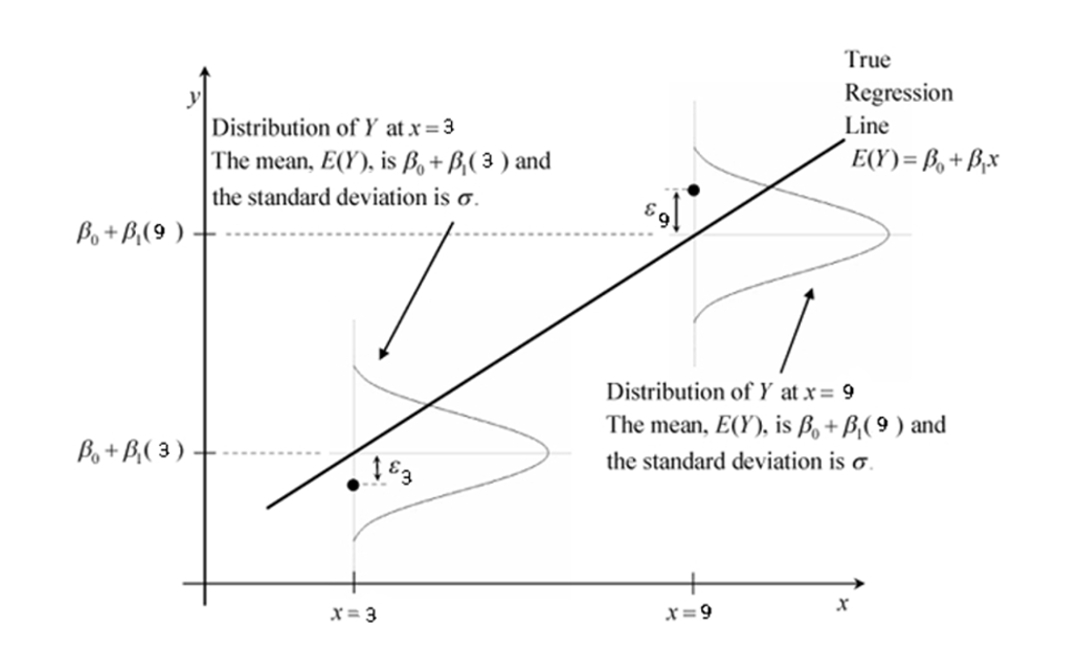
\includegraphics[width=15.03in]{res.std.err}

The formula for the residual standard deviation is:
\[\hat{\sigma}=\sqrt{\frac{\sum r_i^2}{n-p}}\]

where \(n\) is the sample size and \(p\) is the number of predictors + 1, or the number of coefficients estimated by the model. As you can see it is a sort of average of the squared residual -- divided by the number of points in the sample minus the number of parameters to be estimated.

\fcolorbox{black}{white}{\color{black}
\begin{minipage}[c][5cm][t]{\textwidth}
\sffamily\fboxrule.1em\fboxsep1em
Q: What happens to $\hat{\sigma}$ as the number of parameters p increases for fixed sample size n?\\
\end{minipage}}

\fcolorbox{black}{white}{\color{black}
\begin{minipage}[c][5cm][t]{\textwidth}
\sffamily\fboxrule.1em\fboxsep1em
Q: What happens as the sample size n increases for a fixed number of parameters p?
\end{minipage}}

\hypertarget{the-r-squared}{%
\subsubsection{The R-squared}\label{the-r-squared}}

The \(R^2\) is a commonly used regression \emph{diagnostic}, i.e.~it helps us decide whether the linear model fits the data well.

\fcolorbox{black}{white}{\color{black}
\begin{minipage}[c][15cm][t]{\textwidth}
\sffamily\fboxrule.1em\fboxsep1em
\color{white}xxxxxxxxxxxx\color{black}
\end{minipage}}

\textbf{You could try the Least squares estimate exercises in the back of the book now}

\hypertarget{workshop-3-simple-linear-regression}{%
\section{Workshop 3: Simple linear regression}\label{workshop-3-simple-linear-regression}}

\hypertarget{learning-outcomes-4}{%
\subsection{Learning outcomes}\label{learning-outcomes-4}}

Perform some exploratory analysis, perform simple linear regressions in \texttt{R} and interpret the coefficients.

Basic understanding of the residual assumptions and the residual plots.

Basic understanding of the the \(R^2\) and the residual standard deviation as ``goodness of fit'' measures.

I will be using both the command \texttt{ggplot()} from the ``ggplot2'' package and \texttt{plot()}. Specifically residual plots the \texttt{plot()} command in the ``base'' package in \texttt{R} is quicker. For those who have difficulty installing or accessing the ``ggplot2'' package on your PCs or laptops, I include the code for using \texttt{plot()} in some of the plots below but it is generally commented out.

\emph{Note}: Adding a ``\#'' at the beginning of a line \texttt{R} code \emph{comments is out}, i.e.~you can see it but \texttt{R} ignores

\hypertarget{preamble-1}{%
\subsection{Preamble}\label{preamble-1}}

Remember to load packages below if you can

\begin{Shaded}
\begin{Highlighting}[]
\FunctionTok{library}\NormalTok{(arm)}
\FunctionTok{library}\NormalTok{(ggplot2)}
\end{Highlighting}
\end{Shaded}

\hypertarget{data}{%
\subsection{Data}\label{data}}

For this and some future classes we'll be using the Stats study habits dataset. This is based on a questionnaire of LSE stats students over the course of 3 years. The questionnaire asked about student's study habits -- how often, whether in groups or alone, how they did in tests etc. The responses to some of these questions were then transformed into 8 study skill scores the sum of which we use as a predictor variable here. The outcome of interest is the grade (out of 100) in the stats exam.

\begin{longtable}[]{@{}
  >{\centering\arraybackslash}p{(\columnwidth - 4\tabcolsep) * \real{0.1259}}
  >{\centering\arraybackslash}p{(\columnwidth - 4\tabcolsep) * \real{0.0963}}
  >{\raggedright\arraybackslash}p{(\columnwidth - 4\tabcolsep) * \real{0.7778}}@{}}
\toprule()
\begin{minipage}[b]{\linewidth}\centering
Name
\end{minipage} & \begin{minipage}[b]{\linewidth}\centering
Type
\end{minipage} & \begin{minipage}[b]{\linewidth}\raggedright
Description
\end{minipage} \\
\midrule()
\endhead
Interesting & binary & Is stats interesting? 1 - yes, 0 - no \\
Study Skills & continuous & 0-56 Total study skills - higher is more skills \\
Grade & continuous & grades in stats exam out of 100 \\
Enjoy & binary & Do you enjoy stats? 1-yes, 0 - no \\
A-level & continuous & grades in stat/maths A-level out of 7 \\
\bottomrule()
\end{longtable}

Let's load the data and check it looks OK.

\begin{Shaded}
\begin{Highlighting}[]
\NormalTok{Study\_habits}\OtherTok{\textless{}{-}}\FunctionTok{read.csv}\NormalTok{(}\StringTok{"Stats\_study\_habits\_slr.csv"}\NormalTok{)}
\FunctionTok{head}\NormalTok{(Study\_habits)}
\FunctionTok{summary}\NormalTok{(Study\_habits)}
\end{Highlighting}
\end{Shaded}

\fcolorbox{black}{white}{\color{black}
\begin{minipage}[c][4cm][t]{\textwidth}
\sffamily\fboxrule.1em\fboxsep1em
Q: What is the range of A-level? Study.Skills?\\
\\
\\
Q: What is the median Grade?
\\
\\
Q: What is the proportion of students who enjoy statistics? 
\\
\\
Q: What is the proportion of students who are interested in statistics?
\end{minipage}}

\hypertarget{binary-predictors-interesting}{%
\subsection{Binary predictors -- Interesting}\label{binary-predictors-interesting}}

We'll start with one binary predictor: Interesting.

Before we start with the analysis think briefly about what relationship you expect to see between Interesting and Grades. You should get into the habit of doing this. It helps to engage with the data so that you don't blindly accept whatever output \texttt{R} gives you. However you also need to be aware of the fact that relationships in simple linear regression, as expressed by regression coefficients, may change in both size and direction when more than one predictor is introduced.

\fcolorbox{black}{white}{\color{black}
\begin{minipage}[c][2cm][t]{\textwidth}
\sffamily\fboxrule.1em\fboxsep1em
Q: What do you expect the relationship between Interesting and Grade to be?
\end{minipage}}

Next let's plot the data. Below is a boxplot that shows how the Grades are distributed amongst those who do and don't find stats interesting.

\begin{Shaded}
\begin{Highlighting}[]
\CommentTok{\#R base package plot}
\CommentTok{\#with(Study\_habits,boxplot(Grade\textasciitilde{}Interesting, xlab="Interesting", ylab="Grade"))}
\DocumentationTok{\#\#ggplot2}
\FunctionTok{ggplot}\NormalTok{(Study\_habits, }\FunctionTok{aes}\NormalTok{(}\AttributeTok{x=}\FunctionTok{factor}\NormalTok{(Interesting), }\AttributeTok{y=}\NormalTok{Grade)) }\SpecialCharTok{+} \FunctionTok{geom\_boxplot}\NormalTok{()}
\end{Highlighting}
\end{Shaded}

\begin{center}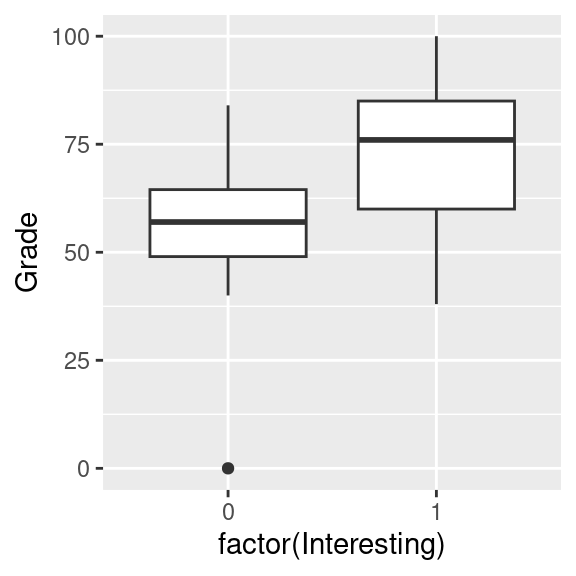
\includegraphics{_main_files/figure-latex/unnamed-chunk-67-1} \end{center}

\fcolorbox{black}{white}{\color{black}
\begin{minipage}[c][2cm][t]{\textwidth}
\sffamily\fboxrule.1em\fboxsep1em
Q:What do you infer from the plot?\\
\end{minipage}}

\newpage

Let's run a regression using \texttt{lm()}

\begin{Shaded}
\begin{Highlighting}[]
\NormalTok{grade.interesting.lm}\OtherTok{\textless{}{-}}\FunctionTok{lm}\NormalTok{(Grade}\SpecialCharTok{\textasciitilde{}}\NormalTok{Interesting,}\AttributeTok{data=}\NormalTok{Study\_habits)}
\FunctionTok{display}\NormalTok{(grade.interesting.lm)}
\end{Highlighting}
\end{Shaded}

\begin{verbatim}
## lm(formula = Grade ~ Interesting, data = Study_habits)
##             coef.est coef.se
## (Intercept) 57.47     2.39  
## Interesting 15.26     2.91  
## ---
## n = 133, k = 2
## residual sd = 15.68, R-Squared = 0.17
\end{verbatim}

Formally: E\((\)Grade\()=57.5+15.3 Interesting\)

The model tells us about the \textbf{difference} in Grades between people who say they find stats interesting vs those who don't.

Plug Interesting=0 into the regression and you get the \textbf{intercept} 57.5, i.e.~the predicted Grade for students who do not find statistics interesting. Plug Interesting=1 into the equation you get \(57.5+15.3=72.8\) which is the predicted Grade for students who find statistics interesting. 15.3 is the \textbf{slope} and tells us that students who find statistics interesting have \textbf{on average} a 15.3 higher Grade than students who do not.

\hypertarget{continuous-predictor-study.skills}{%
\subsection{Continuous predictor -- Study.Skills}\label{continuous-predictor-study.skills}}

We now use a single continuous predictor: Study.Skills. Study.Skills is the sum of the scores obtained by students for a number of study skill related variables. The higher it is the more study skills the student has. The maximum possible is 56 although no-one in the sample attained that.

\fcolorbox{black}{white}{\color{black}
\begin{minipage}[c][2cm][t]{\textwidth}
\sffamily\fboxrule.1em\fboxsep1em
Q:What do you anticipate the relationship between Study.Skills and Grades to be?
\end{minipage}}

\begin{Shaded}
\begin{Highlighting}[]
\CommentTok{\#R base package}
\CommentTok{\#with(Study\_habits, plot(Study.Skills,Grade,pch=4))}
\FunctionTok{ggplot}\NormalTok{(Study\_habits, }\FunctionTok{aes}\NormalTok{(}\AttributeTok{x=}\NormalTok{Study.Skills, }\AttributeTok{y=}\NormalTok{Grade))}\SpecialCharTok{+} \FunctionTok{geom\_point}\NormalTok{()}
\end{Highlighting}
\end{Shaded}

\begin{center}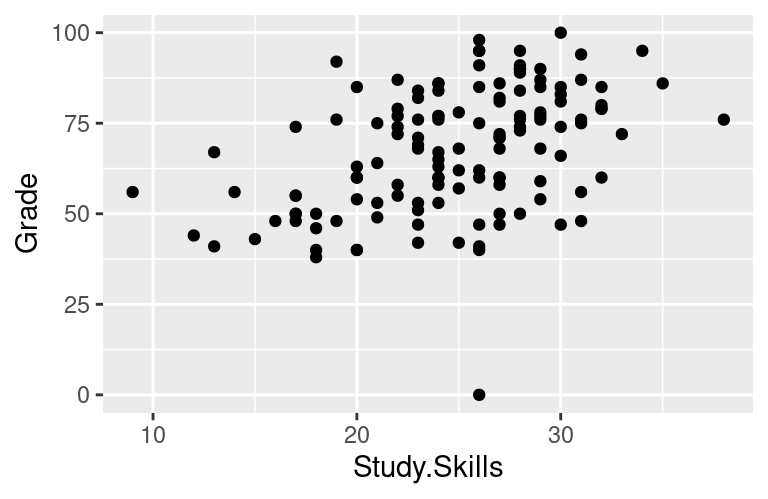
\includegraphics{_main_files/figure-latex/unnamed-chunk-69-1} \end{center}

\fcolorbox{black}{white}{\color{black}
\begin{minipage}[c][2cm][t]{\textwidth}
\sffamily\fboxrule.1em\fboxsep1em
Q: What do you infer from the plot?
\end{minipage}}

\color{white} zzzzzz \color{black} \fcolorbox{black}{lightgray!20!white}{\color{black}
\begin{minipage}[c][6cm][t]{12.5cm}
The "ggplot2" package is part of the "tidyverse" approach to coding in \texttt{R} which is becoming increasingly popular. Instead of having a function and adding all the arguments inside it, it has a core command \texttt{ggplot()} which defines the data and the variables (\texttt{x,y,fill,colour}) and then additional function follow with a \texttt{+}\\
\\
We've seen that in both the cases above the \texttt{ggplot()}  command was similar, with just the \texttt{x} changing value. The first plot was a boxplot so \texttt{+ geom\_boxplot()} was added. The second plot was a scatterplot so \texttt{+ geom\_point()} was added.\\
\\
In order to make sure the whole line of code is visible in the output on the page in front of you, from now on, I assign a name (\texttt{p1}) to the plot I create in ``ggplot()`` and then add arguments to \texttt{p1} in subsequent lines.

\end{minipage}}

Now for the regression:

\begin{Shaded}
\begin{Highlighting}[]
\NormalTok{grade.studyskills.lm}\OtherTok{\textless{}{-}}\FunctionTok{lm}\NormalTok{(Grade}\SpecialCharTok{\textasciitilde{}}\NormalTok{Study.Skills, }\AttributeTok{data=}\NormalTok{Study\_habits)}
\FunctionTok{display}\NormalTok{(grade.studyskills.lm)}
\end{Highlighting}
\end{Shaded}

\begin{verbatim}
## lm(formula = Grade ~ Study.Skills, data = Study_habits)
##              coef.est coef.se
## (Intercept)  30.77     6.70  
## Study.Skills  1.49     0.26  
## ---
## n = 133, k = 2
## residual sd = 15.47, R-Squared = 0.20
\end{verbatim}

Formally E\((\)Grade\()=38.8+1.5Study.Skills\)

The model tells us by how much the \emph{average} Grade changes when Study.Skills increases by \emph{one}.

Plug Study.Skills=0 into the regression equation, this gives you the \textbf{intercept}: 38.8 which is the predicted score for students who have a 0 Study.Skills score. \(30.8+1.5=32.3\) is the predicted score for students who have value 1 Study.Skills score. \(30.8+1.5\times10=45.8\) is the predicted score for a student with Study.Skills score of 10.
1.5 is the \textbf{slope} and tells us that the predicted Grade increases \textbf{on average} by 1.5 for an increase of 1 in the study skills score.

\fcolorbox{black}{white}{\color{black}
\begin{minipage}[c][3cm][t]{\textwidth}
\sffamily\fboxrule.1em\fboxsep1em
Q: Are any students likely to have a Study skills score of 0? \\
\\
\\
Q: If not, how is the intercept to be interpreted?

\end{minipage}}

\hypertarget{adding-a-regression-line-to-the-plot}{%
\subsubsection{Adding a regression line to the plot}\label{adding-a-regression-line-to-the-plot}}

\begin{Shaded}
\begin{Highlighting}[]
\NormalTok{p1}\OtherTok{\textless{}{-}} \FunctionTok{ggplot}\NormalTok{(Study\_habits, }\FunctionTok{aes}\NormalTok{(}\AttributeTok{x=}\NormalTok{Study.Skills, }\AttributeTok{y=}\NormalTok{Grade))}\SpecialCharTok{+} \FunctionTok{geom\_point}\NormalTok{() }
\NormalTok{p1}\OtherTok{\textless{}{-}}\NormalTok{ p1 }\SpecialCharTok{+} \FunctionTok{geom\_smooth}\NormalTok{(}\AttributeTok{method=}\StringTok{"lm"}\NormalTok{,}\AttributeTok{fill=}\ConstantTok{NA}\NormalTok{)}
\NormalTok{p1}
\end{Highlighting}
\end{Shaded}

\begin{verbatim}
## `geom_smooth()` using formula 'y ~ x'
\end{verbatim}

\begin{center}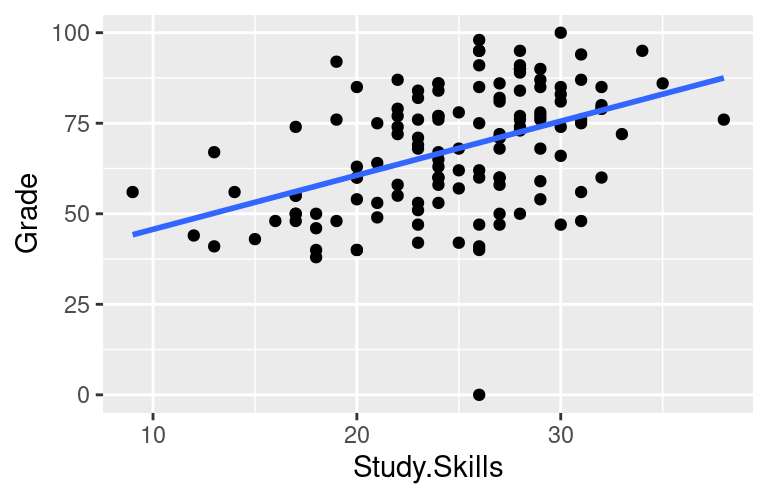
\includegraphics{_main_files/figure-latex/unnamed-chunk-71-1} \end{center}

\color{white} zzzzzz \color{black} \fcolorbox{black}{lightgray!20!white}{\color{black}
\begin{minipage}[c][4cm][t]{12.5cm}
If not using the "ggplot2" package, you can use the \texttt{abline()} function to do something similar. It can be used in 3 modes:
\\
1. Adding a regression line \texttt{abline(grade.studyskills.lm)}\\
2. Adding a line using the intercept (\texttt{a}) and the slope (\texttt{b}) \\
\texttt{abline(a=40,b=1.5, lty=2)}\\
3. Adding vertical or horizontal lines \texttt{abline(v=20,lty=3), abline(h=60,lty=4) }\\
\\
\texttt{lty} is a graphical parameter that specifies the line type (dashed=2, solid=1). If you Google "lty R" you'll see a list.
\end{minipage}}

\begin{Shaded}
\begin{Highlighting}[]
\CommentTok{\#with(Study\_habits, plot(Study.Skills,Grade,pch=4))}
\CommentTok{\#abline(grade.studyskills.lm)}
\CommentTok{\#abline(a=40,b=1.5, lty=2)}
\CommentTok{\#abline(v=mean(Study\_habits$Study.Skills),lty=3)}
\CommentTok{\#abline(h=mean(Study\_habits$Grade),lty=4)}
\end{Highlighting}
\end{Shaded}

\hypertarget{residual-assumptions}{%
\subsection{Residual Assumptions}\label{residual-assumptions}}

The assumptions we discuss below are about the error in a regression, that is, the difference between the ``true'' regression line and the observed points. However we don't observe the error directly because all we have is the estimated line so we use the residuals as a proxy. Note that assumptions about the error are mirrored by assumptions about the outcome as the residual is the outcome minus a straight line (i.e.~the residual is a linear transformation of the outcome).

\textbf{Normality}

Hypothesis tests all rely on the errors (\(\epsilon\)) being approximately normally distributed in linear regression. If normality does not hold then the hypothesis tests can be invalid.

Predictions also become unreliable if we cannot rely on normality.

It is always important to check \emph{approximate} normality of residuals. Linear regression is still valuable when the residuals aren't normally distributed, but results are less reliable.

Normality is checked using:

\begin{itemize}
\tightlist
\item
  The histogram of the residuals.
\item
  The Q-Q plot.
\end{itemize}

\textbf{Independence}

The error terms have to be independent of one another. Consider the following two situations:

\begin{enumerate}
\def\labelenumi{\arabic{enumi}.}
\tightlist
\item
  Data are daily temperatures measured outside Columbia house in the MT 2018
\item
  Data are number of beers sold from a beach shack in Australia and the number of shark attacks in the area over 10 years
\end{enumerate}

\emph{1. Temperatures}

If we regress temperature on day from the first to the last day of the MT 2018 the residuals will be correlated.

\fcolorbox{black}{white}{\color{black}
\begin{minipage}[c][3cm][t]{\textwidth}
\sffamily\fboxrule.1em\fboxsep1em
Q: Why are the residuals correlated?
\end{minipage}}

We don't look at time series in this course so we will not come across this type of problem directly. However independence of this type can be checked by plotting the errors against time -- you will expect to see some sort of seasonal pattern.

\emph{2. Beer/Sharks}

If we regress shark attacks per summer on number of beers sold we see that the two are correlated. However the regression will also result in correlated errors.

\fcolorbox{black}{white}{\color{black}
\begin{minipage}[c][5cm][t]{\textwidth}
\sffamily\fboxrule.1em\fboxsep1em
Q: Why are the residuals correlated?
\end{minipage}}

This type of problem can sometimes be avoided by trying to understand how variables in a data set are related and whether there are any predictor variables that might take the role of \emph{confounding} variables. I.e. variables that are somehow (causally?) related to the other predictors such that omitting them introduces dependence and therefore bias into the regression.

If we include data on them in the regression we may be able to overcome the problem. Including these variables can even result in a change of sign! Other times we simply do not have data on these variables and must accept that our analysis is likely to be incorrect to some extent. These variables are also called, lurking, omitted. There is an exercise in the back of the course notes to investigate the effect of confounding on estimates of regression coefficients.

\textbf{Constant Variance}

In order for linear regression to be useful we must assume that the errors have a common variance -- i.e.~there is no \emph{heteroscedasticity}. If this assumption is violated then our estimates for standard errors become unreliable as do Hypothesis tests.

Often when there is lack of common variance this can be addressed either by transforming the data or by using non-linear models. We check heteroscedasticity by using:

\begin{itemize}
\tightlist
\item
  The plot of the fitted values vs the residuals

  \begin{itemize}
  \tightlist
  \item
    if this displays a funnel shape
  \item
    if this displays a non-linear relationship
  \end{itemize}
\end{itemize}

then there is evidence of heteroscedasticity.

\textbf{Zero expectation}

The error terms should have a 0 mean. This assumption holds approximately with least squares estimation if the relationships are linear (it's designed that way). If relationships are non-linear then it won't hold. In practice the mean of the residuals will never be exactly 0, however it will be as small as possible.

\hypertarget{residual-plots}{%
\subsubsection{Residual plots}\label{residual-plots}}

The plots used to check the residual assumptions are called \emph{residual plots}. We want 3 plots so we ask for a 2 by 2 grid using \texttt{par(mfrow=c(r,c))} (3 in a row or in a column makes plots look squashed or takes up too much room). For residual plots we use the \texttt{plot()} function as it easily produces residual plots when it is passed a linear model.

\begin{Shaded}
\begin{Highlighting}[]
\FunctionTok{par}\NormalTok{(}\AttributeTok{mfrow=}\FunctionTok{c}\NormalTok{(}\DecValTok{2}\NormalTok{,}\DecValTok{2}\NormalTok{))}
\FunctionTok{plot}\NormalTok{(grade.studyskills.lm, }\AttributeTok{which=}\FunctionTok{c}\NormalTok{(}\DecValTok{1}\NormalTok{,}\DecValTok{2}\NormalTok{))}
\FunctionTok{hist}\NormalTok{(}\FunctionTok{rstandard}\NormalTok{(grade.studyskills.lm), }\AttributeTok{freq =} \ConstantTok{FALSE}\NormalTok{ , }
     \AttributeTok{main=}\StringTok{"Histogram of standardised residuals"}\NormalTok{, }
     \AttributeTok{cex.main=}\FloatTok{0.8}\NormalTok{, }\AttributeTok{xlab=}\StringTok{"Standardised residuals"}\NormalTok{)}
\end{Highlighting}
\end{Shaded}

\begin{center}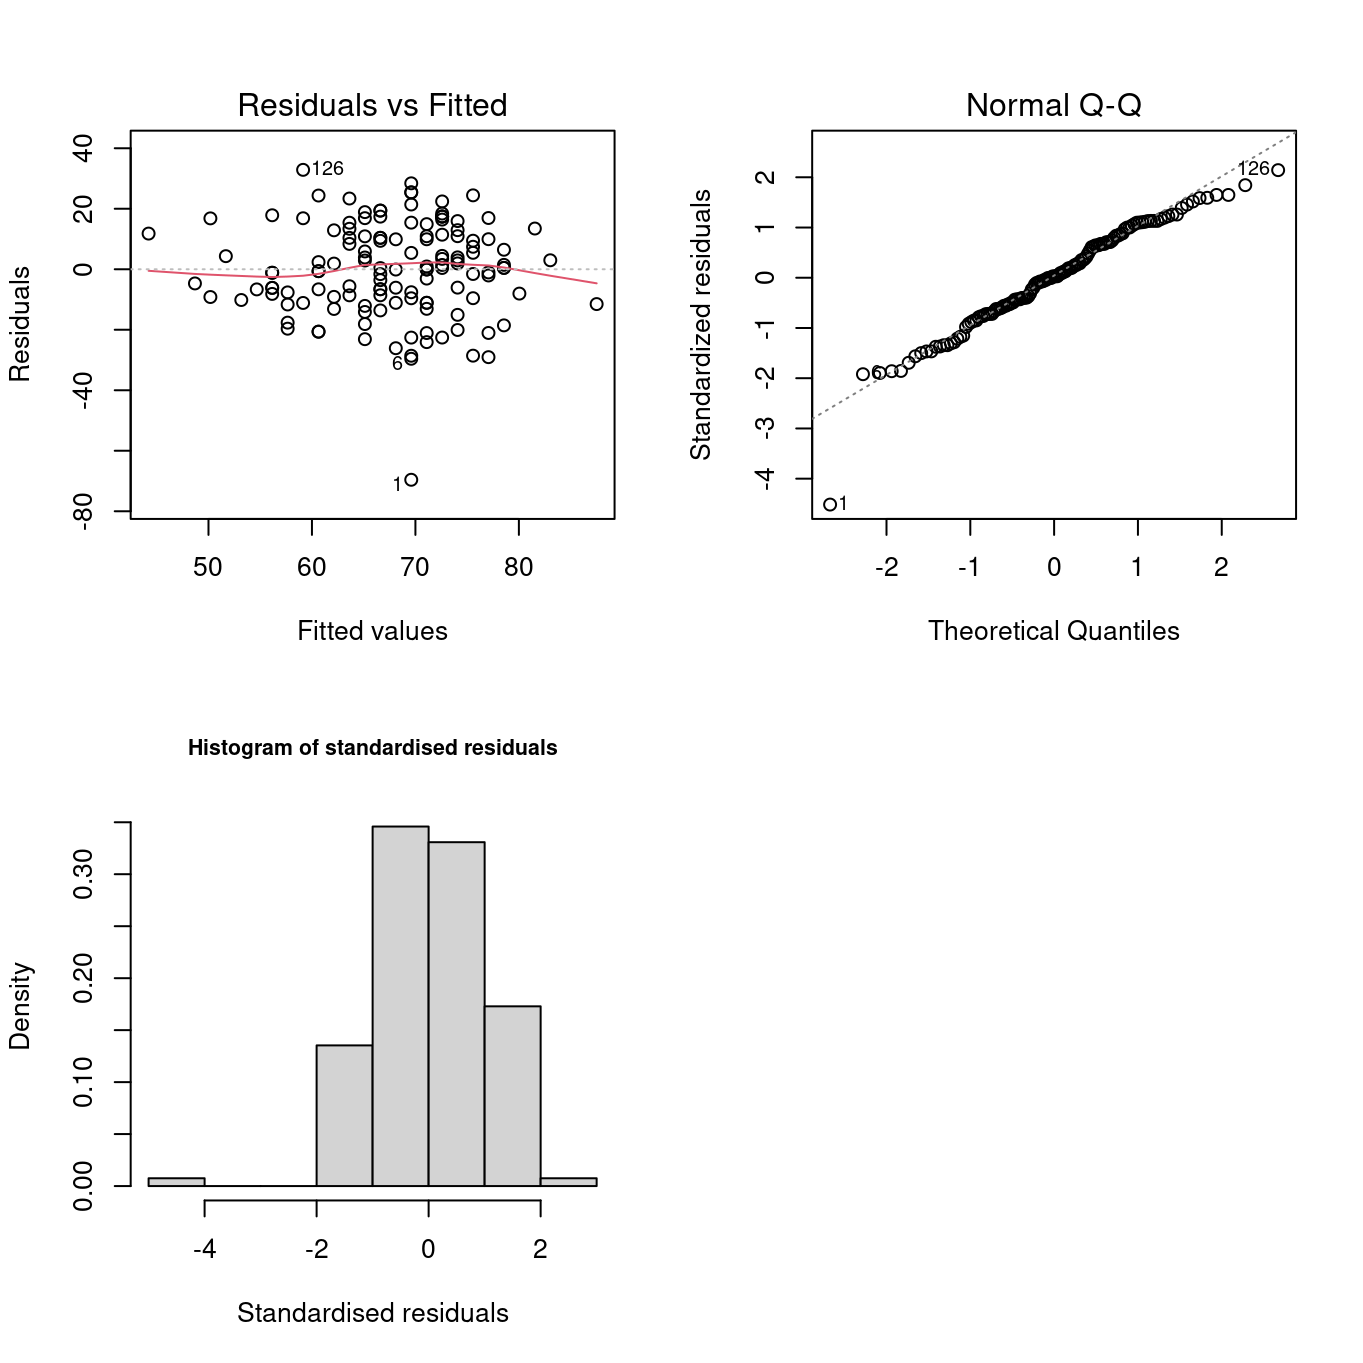
\includegraphics{_main_files/figure-latex/unnamed-chunk-73-1} \end{center}

Let's go through this code:

\begin{itemize}
\tightlist
\item
  \texttt{plot(grade.studyskills.lm)} produces 4 plots. We only want 2 of them, the residual vs fitted and the Q-Q plot
\item
  As these are the 1st two we add an argument \texttt{which=c(1,2)}
\item
  \texttt{hist(x)} produces a histogram of x
\item
  \texttt{rstandard(grade.studyskills.lm)} are the standardised residuals
\item
  \texttt{main="Histogram\ of\ residuals"} is the title of the plot -- Histogram of residuals
\item
  \texttt{font.main=1} determines the size of the font of the title
\item
  \texttt{xlab="Residuals"} says that the x label -- Residuals
\item
  \texttt{probability=TRUE} gives the probability histogram rather than the frequency histogram
\end{itemize}

\textbf{Exercise}

For the three residual plots above, do you think the residual assumptions hold? If not, why not?

\fcolorbox{black}{white}{\color{black}
\begin{minipage}[c][5cm][t]{\textwidth}
\sffamily\fboxrule.1em\fboxsep1em
Normality:\\
\\
\\
\\
\\
\\
\\
\\
Constant variance:\\

\end{minipage}}

\hypertarget{some-goodness-of-fit-statistics-residual-standard-deviation-and-r-squared}{%
\subsection{Some goodness of fit statistics: Residual standard deviation and R-squared}\label{some-goodness-of-fit-statistics-residual-standard-deviation-and-r-squared}}

Let's have another look at the output from \texttt{display}:

\begin{Shaded}
\begin{Highlighting}[]
\NormalTok{grade.lm}\FloatTok{.0}\OtherTok{\textless{}{-}}\FunctionTok{lm}\NormalTok{(Grade}\SpecialCharTok{\textasciitilde{}}\NormalTok{Study.Skills, }\AttributeTok{data=}\NormalTok{Study\_habits)}
\FunctionTok{display}\NormalTok{(grade.lm}\FloatTok{.0}\NormalTok{)}
\end{Highlighting}
\end{Shaded}

\begin{verbatim}
## lm(formula = Grade ~ Study.Skills, data = Study_habits)
##              coef.est coef.se
## (Intercept)  30.77     6.70  
## Study.Skills  1.49     0.26  
## ---
## n = 133, k = 2
## residual sd = 15.47, R-Squared = 0.20
\end{verbatim}

At the bottom of the output are two statistics: the residual standard deviation (\texttt{residual\ sd}) and the \(R^2\) (\texttt{R-Squared}). These statistics are crude (but often effective) measures of how well the model fits and/or explains the data.

The residual standard deviation is the standard deviation of the estimated regression line. It should be smaller than the range of the outcome:

In our case max(Grade)-min(Grade)=100 and \(\hat{\sigma}\)=15.47

\fcolorbox{black}{white}{\color{black}
\begin{minipage}[c][3cm][t]{\textwidth}
\sffamily\fboxrule.1em\fboxsep1em
Q: Interpret the residual standard deviation in this example:
\end{minipage}}

The lower the R-squared the better the fit of the line. In our case it is 0.20 so 20\%.

\fcolorbox{black}{white}{\color{black}
\begin{minipage}[c][3cm][t]{\textwidth}
\sffamily\fboxrule.1em\fboxsep1em
Q: Comment on the R-squared in this example:
\end{minipage}}

\#\#\#For the \texttt{plot()} command only:

\color{white} zzzzzz \color{black} \fcolorbox{black}{lightgray!20!white}{\color{black}
\begin{minipage}[c][2cm][t]{12.5cm}
Often you will want to put more than one graph on the same page. If you use \texttt{plot()} then you'll need to put \texttt{par(mfrow=c(num.rows,num.columns))} before the plots. \\
Note that if you close the plot then the \texttt{par()} option gets forgotten.  \\
For example:\\
\end{minipage}}

\begin{Shaded}
\begin{Highlighting}[]
\FunctionTok{par}\NormalTok{(}\AttributeTok{mfrow=}\FunctionTok{c}\NormalTok{(}\DecValTok{2}\NormalTok{,}\DecValTok{1}\NormalTok{))}
\FunctionTok{plot}\NormalTok{(}\FunctionTok{seq}\NormalTok{(}\DecValTok{1}\NormalTok{,}\DecValTok{10}\NormalTok{),}\FunctionTok{seq}\NormalTok{(}\DecValTok{1}\NormalTok{,}\DecValTok{10}\NormalTok{))}
\FunctionTok{plot}\NormalTok{(}\FunctionTok{seq}\NormalTok{(}\DecValTok{1}\NormalTok{,}\DecValTok{10}\NormalTok{),}\FunctionTok{seq}\NormalTok{(}\DecValTok{1}\NormalTok{,}\DecValTok{10}\NormalTok{),}\AttributeTok{col=}\StringTok{"red"}\NormalTok{)}
\end{Highlighting}
\end{Shaded}

Then try:

\begin{Shaded}
\begin{Highlighting}[]
\FunctionTok{par}\NormalTok{(}\AttributeTok{mfrow=}\FunctionTok{c}\NormalTok{(}\DecValTok{1}\NormalTok{,}\DecValTok{2}\NormalTok{))}
\FunctionTok{plot}\NormalTok{(}\FunctionTok{seq}\NormalTok{(}\DecValTok{1}\NormalTok{,}\DecValTok{10}\NormalTok{),}\FunctionTok{seq}\NormalTok{(}\DecValTok{1}\NormalTok{,}\DecValTok{10}\NormalTok{))}
\FunctionTok{plot}\NormalTok{(}\FunctionTok{seq}\NormalTok{(}\DecValTok{1}\NormalTok{,}\DecValTok{10}\NormalTok{),}\FunctionTok{seq}\NormalTok{(}\DecValTok{1}\NormalTok{,}\DecValTok{10}\NormalTok{),}\AttributeTok{col=}\StringTok{"red"}\NormalTok{)}
\end{Highlighting}
\end{Shaded}

\hypertarget{lecture-4-multiple-linear-regression-part-1}{%
\section{Lecture 4: Multiple linear regression Part 1}\label{lecture-4-multiple-linear-regression-part-1}}

\hypertarget{learning-outcomes-5}{%
\subsection{Learning outcomes:}\label{learning-outcomes-5}}

Extending linear regression to include one binary and one continuous predictor

Understanding interactions between a binary and a continuous predictor in multiple linear regression

\hypertarget{data-1}{%
\subsection{Data}\label{data-1}}

In this lecture we'll use the Study Skills data set again but we'll use \emph{two} predictors. \texttt{Interesting} and \texttt{Study.Skills}.

\begin{longtable}[]{@{}
  >{\centering\arraybackslash}p{(\columnwidth - 4\tabcolsep) * \real{0.1259}}
  >{\centering\arraybackslash}p{(\columnwidth - 4\tabcolsep) * \real{0.0963}}
  >{\raggedright\arraybackslash}p{(\columnwidth - 4\tabcolsep) * \real{0.7778}}@{}}
\toprule()
\begin{minipage}[b]{\linewidth}\centering
Name
\end{minipage} & \begin{minipage}[b]{\linewidth}\centering
Type
\end{minipage} & \begin{minipage}[b]{\linewidth}\raggedright
Description
\end{minipage} \\
\midrule()
\endhead
Interesting & binary & Is stats interesting? 1 - yes , 0 - no \\
Study Skills & continuous & 0-56 Total study skills - higher is more skills \\
Grade & continuous & grades in stats exam out of 100 \\
\bottomrule()
\end{longtable}

\begin{Shaded}
\begin{Highlighting}[]
\NormalTok{Study\_habits}\OtherTok{\textless{}{-}}\FunctionTok{read.csv}\NormalTok{(}\StringTok{"Stats\_study\_habits\_mlr.csv"}\NormalTok{)}
\FunctionTok{head}\NormalTok{(Study\_habits)}
\end{Highlighting}
\end{Shaded}

With two predictors the ``true'' regression looks like this:
\[ y = \beta_0+ \beta_1 x_1 + \beta_2 x_2\]
Using our data this becomes:
\[ Grade =  \beta_0 + \beta_1 Study.Skills+ \beta_2 Interesting\]
\fcolorbox{black}{white}{\color{black}
\begin{minipage}[c][5.5cm][t]{\textwidth}
\sffamily\fboxrule.1em\fboxsep1em
Q: Before running the regression, what do you think the signs of $\beta_1$ and $\beta_2$ are?\\
\\
\\
\\
Q: Do you think that Study.Skills and Interesting \textit{interact}? I.e. do you think that students who are interested benefit more/less from having higher study skills that students who are not interested?  By "benefit" I mean "get higher grades".

\end{minipage}}

This is a complex question and I just want you to bear it in mind when we look at subsets regression and interactions later in the lecture.

Let's run the regression. Below are the values for the regression coefficients:

\begin{Shaded}
\begin{Highlighting}[]
\NormalTok{grade.lm}\FloatTok{.1}\OtherTok{\textless{}{-}}\FunctionTok{lm}\NormalTok{(Grade}\SpecialCharTok{\textasciitilde{}}\NormalTok{Study.Skills}\SpecialCharTok{+}\NormalTok{Interesting,}\AttributeTok{data=}\NormalTok{Study\_habits)}
\FunctionTok{coef}\NormalTok{(grade.lm}\FloatTok{.1}\NormalTok{)}
\end{Highlighting}
\end{Shaded}

\begin{verbatim}
##  (Intercept) Study.Skills  Interesting 
##    31.975960     1.124188    12.041984
\end{verbatim}

The regression looks like this:
\[ E(Grade) =31.98 + 1.12 Study.Skills + 12.04 Interesting \]

\#\#Plots for multiple predictors

We saw how to plot this data for one predictor. Below is how it can be plotted for a continuous and a binary (or categorical) predictor.

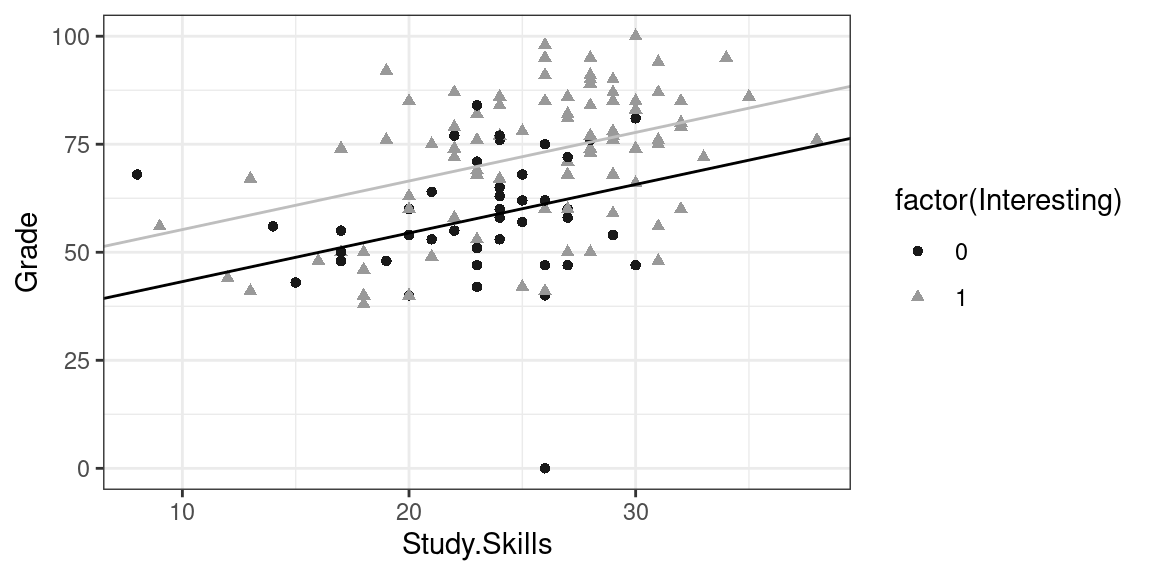
\includegraphics{_main_files/figure-latex/unnamed-chunk-79-1.pdf}

\fcolorbox{black}{white}{\color{black}
\begin{minipage}[c][1.5cm][t]{\textwidth}
\sffamily\fboxrule.1em\fboxsep1em
Q: What do you notice about the slopes of the two lines? 
\end{minipage}}

The regression line above is using the value of interesting to change the intercept only.
So, when \texttt{Interesting}=0 the line is
\[ E(Grade) =31.98 + 1.12 Study.Skills\]
But when \texttt{Interesting}=1 the line is
\[ E(Grade)  =31.98 + 1.12 Study.Skills + 12.04\]
\[ = 44.02 + 1.12 Study.Skills\]
\fcolorbox{black}{white}{\color{black}
\begin{minipage}[c][3cm][t]{\textwidth}
\sffamily\fboxrule.1em\fboxsep1em
Q: Do you think that imposing the same slope is sensible? Justify your answer based on the data/knowledge
\end{minipage}}

\#\#Interpreting coefficients

Looking at the regression again:

\[ E(Grade) =31.98 + 1.12 Study.Skills + 12.04 Interesting \]

\begin{itemize}
\tightlist
\item
  The \emph{intercept}: A students with no study skills (\texttt{Study.Skills}=0) and with no interest in statistics (\texttt{Interesting}=0) has an average predicted \texttt{Grade} of 31.98. Again not very useful as \texttt{Study.Skills}=0 is unlikely.
\item
  The \emph{coefficient} of \texttt{Interesting}: When we look at students who have \emph{the same} level of \texttt{Study.Skills} then those who are interested in statistics are on average getting 12.04 more in their \texttt{Grade} than those who are not interested.
\item
  The \emph{coefficient} of \texttt{Study.Skills}: We expect students to get on average 1.12 more in their \texttt{Grade} for every additional point in \texttt{Study.Skills} score for any level of \texttt{Interesting}
\end{itemize}

The basic idea behind interpreting coefficients is thinking how changing one predictor changes the average outcome \emph{while keeping the values/levels of the other predictors the} \textbf{same}.

\#\#\#Subset Regression

We can explore whether the same slope assumption is reasonable by running two separate regressions: one for those who are interested and another for those who are not:

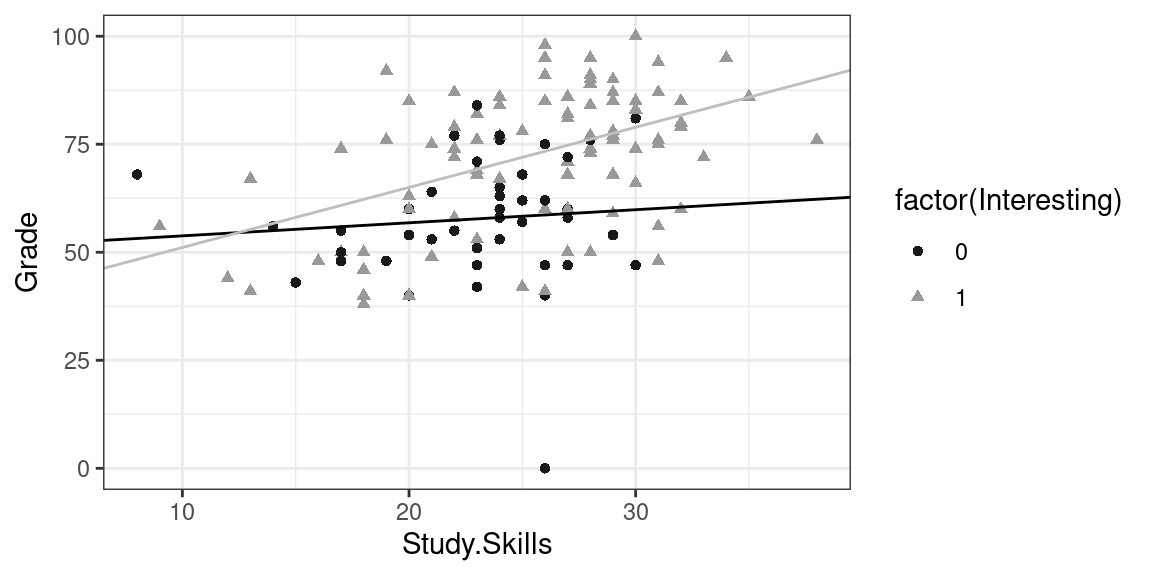
\includegraphics{_main_files/figure-latex/unnamed-chunk-80-1.pdf}

\fcolorbox{black}{white}{\color{black}
\begin{minipage}[c][2cm][t]{\textwidth}
\sffamily\fboxrule.1em\fboxsep1em
Q: What do you notice about the lines in this plot as compared to the one above?
\end{minipage}}

From the plot we can see that the slope for the students who are not interested is approximately 0. That means that having a higher study skills score doesn't help them to get better grades in their statistics exam. Students who are interested however do benefit from having a higher study skills score as this slope is positive.

\textbf{So should we always do subset regression?}

\begin{itemize}
\tightlist
\item
  No.~You \emph{should} do if when the interest is in specific subsets/sub populations (e.g.~countries, regions)
\item
  Other times it is not necessary. For example when there are few subsets (e.g.~men vs women)
\item
  Or not every subset is relevant or important
\item
  Often including an \emph{interaction} takes into account differences between subsets.
\end{itemize}

\#\#Interactions

As we saw from the subset regression the slopes of the regression lines for the interested vs un-interested students are quite different. This suggest that being interested has a different effect on the grades of those who are interested and those who are un-interested. We can incorporate this into a single regression using an interaction term: The interaction is the \emph{product} of the predictors:

\[ Grade =  \beta_0 + \beta_1 Study.Skills+ \beta_2 Interesting+ \beta_3 Study.Skills \times Interesting\]

\begin{Shaded}
\begin{Highlighting}[]
\NormalTok{grade.lm.int}\OtherTok{\textless{}{-}}\FunctionTok{lm}\NormalTok{(Grade}\SpecialCharTok{\textasciitilde{}}\NormalTok{Study.Skills}\SpecialCharTok{*}\NormalTok{Interesting,}\AttributeTok{data=}\NormalTok{Study\_habits)}
\FunctionTok{coef}\NormalTok{(grade.lm.int)}
\end{Highlighting}
\end{Shaded}

\begin{verbatim}
##              (Intercept)             Study.Skills              Interesting 
##               50.7798909                0.3025668              -13.5712854 
## Study.Skills:Interesting 
##                1.0883059
\end{verbatim}

\textbf{Group work}

\[ E(Grade) =50.78+ 0.3 Study.Skills -13.57 Interesting + 1.09 Study.Skills \times Interesting \]

\fcolorbox{black}{white}{\color{black}
\begin{minipage}[c][6cm][t]{\textwidth}
\sffamily\fboxrule.1em\fboxsep1em
Q: Using the regression equation above write down two regression lines. One for students who are interested in statistics and one for students who are not interested. Once you have done this, plot the slopes on the scatterplot below.
\end{minipage}}

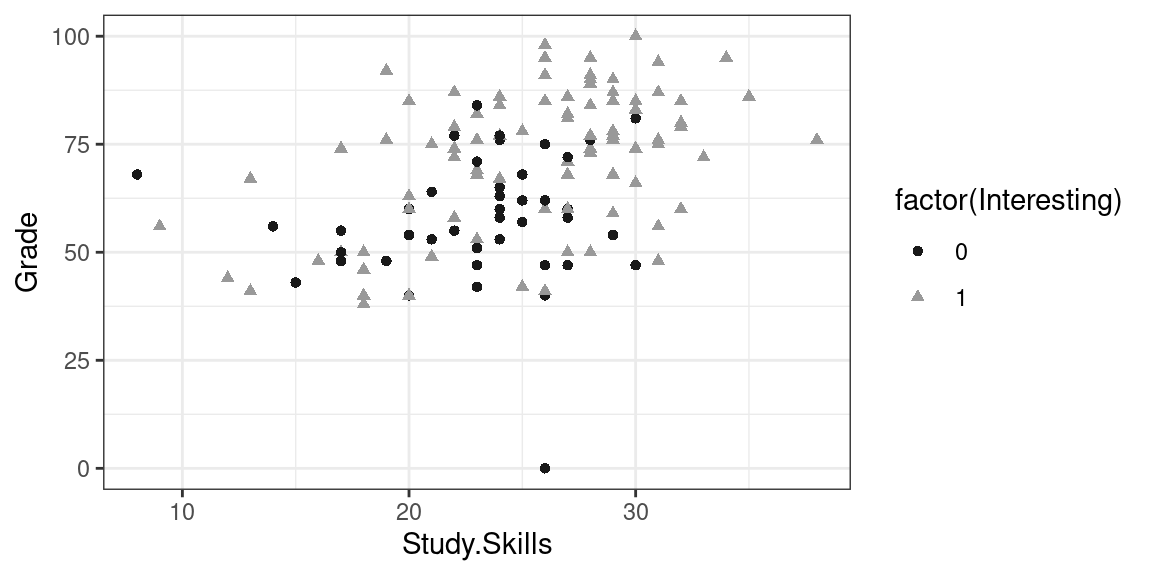
\includegraphics{_main_files/figure-latex/unnamed-chunk-82-1.pdf}

Before, \texttt{Interesting} only contributed to changing the intercept. Now it also contributes to changing the slope.

\#\#\#Interpretation with an interaction

Once we've run a regression with an interaction it is not easy to interpret the parameters \emph{on their own}. The best thing to do is to write down the separate regressions. This is of course more difficult and complex the more interaction terms there are.

However, if you want to try to interpret then:

The \emph{intercept} and the \emph{coefficient} of \texttt{Interesting} alone are not easy to interpret as both require that the value of \texttt{Study.Skills}=0, which as we said is unlikely.

\begin{itemize}
\tightlist
\item
  The coefficient of \texttt{Study.Skills} can be thought of as a comparison between the average \texttt{Grade} for students who are not interested when their study skill score increases by 1.
\item
  The coefficient of the interaction is the change in the coefficient (slope) of \texttt{Study.Skills} between students who aren't interested and those who are.
\end{itemize}

\#\#\#When to add interactions

\begin{itemize}
\tightlist
\item
  Sometimes we are told by subject matter experts that interactions should be included. For example in medical data sex/gender are always included in the model and so are their interactions with other predictors.
\item
  When one or more of the main effects are large, it is a good idea to include interactions at least between the large main effects.
\item
  When some subsets of the data are considered of particular interest (although sometimes subsets regression is better for interpretation if there are many groups -- especially if results need to be explained to subject matter experts who may not be great with equations)
\item
  \emph{Note}: Interactions between two continuous predictors are somewhat harder to understand. They also often lead to multicollinearity and overfitting (discussed later). I would avoid them unless there are strong substantive reasons to add them. In that case there are some interesting ways of visualising them in plots.
\end{itemize}

\hypertarget{workshop-4-multiple-linear-regression}{%
\section{Workshop 4: Multiple Linear Regression}\label{workshop-4-multiple-linear-regression}}

\hypertarget{learning-outcomes-6}{%
\subsection{Learning outcomes}\label{learning-outcomes-6}}

Running a MLR with multiple predictors

Understanding how to plot this to see interactions

Diagnostics Part 2: Adjusted \(R^2\) and F-statistics

In your own time: \texttt{ifelse()}

\hypertarget{preamble-2}{%
\subsection{Preamble}\label{preamble-2}}

Load the following packages:

\begin{Shaded}
\begin{Highlighting}[]
\FunctionTok{library}\NormalTok{(arm)}
\FunctionTok{library}\NormalTok{(ggplot2)}
\end{Highlighting}
\end{Shaded}

\hypertarget{data-2}{%
\subsection{Data}\label{data-2}}

In this workshop we'll use the Study Skills data set again but we'll consider the predictors \texttt{Enjoy} and \texttt{Study.Skills}.

\begin{longtable}[]{@{}
  >{\centering\arraybackslash}p{(\columnwidth - 4\tabcolsep) * \real{0.1259}}
  >{\centering\arraybackslash}p{(\columnwidth - 4\tabcolsep) * \real{0.0963}}
  >{\raggedright\arraybackslash}p{(\columnwidth - 4\tabcolsep) * \real{0.7778}}@{}}
\toprule()
\begin{minipage}[b]{\linewidth}\centering
Name
\end{minipage} & \begin{minipage}[b]{\linewidth}\centering
Type
\end{minipage} & \begin{minipage}[b]{\linewidth}\raggedright
Description
\end{minipage} \\
\midrule()
\endhead
Enjoy & binary & Enjoy, 1 - yes, 0 - no \\
Study Skills & continuous & 0-56 Total study skills - higher is more skills \\
Grade & continuous & grades in stats exam out of 100 \\
\bottomrule()
\end{longtable}

\begin{Shaded}
\begin{Highlighting}[]
\NormalTok{Study\_habits}\OtherTok{\textless{}{-}}\FunctionTok{read.csv}\NormalTok{(}\StringTok{"Stats\_study\_habits\_mlr.csv"}\NormalTok{)}
\FunctionTok{head}\NormalTok{(Study\_habits, }\DecValTok{4}\NormalTok{)}
\end{Highlighting}
\end{Shaded}

\begin{verbatim}
##   Interesting Enjoy A.Level Study.Skills Grade
## 1           1     1       6           18    38
## 2           1     0       6           18    40
## 3           0     0       6           20    40
## 4           1     0       6           20    40
\end{verbatim}

The equation is:
\[ y = \beta_0+ \beta_1 x_1 + \beta_2 x_2\]
Or in our case
\[ Grade =  \beta_0 + \beta_1 Study.Skills+ \beta_2 Enjoy\]

\fcolorbox{black}{white}{\color{black}
\begin{minipage}[c][3.55cm][t]{\textwidth}
\sffamily\fboxrule.1em\fboxsep1em
Q: Before running the regression, what do you think the signs of $\beta_1$ and $\beta_2$ are?\\
\\
\\
Q: Do you think that ``Study.Skills`` and ``Enjoy`` \textit{interact}? I.e. do you think that students who enjoy statistics get higher(lower) grades by having higher study skills that students who do not enjoy statistics?

\end{minipage}}
\newpage

Let's run the regression to see what the least squares \emph{estimates} \(\hat{\beta}\) are.

\begin{Shaded}
\begin{Highlighting}[]
\NormalTok{grade.lm}\FloatTok{.1}\OtherTok{\textless{}{-}}\FunctionTok{lm}\NormalTok{(Grade}\SpecialCharTok{\textasciitilde{}}\NormalTok{Study.Skills}\SpecialCharTok{+}\NormalTok{Enjoy,}\AttributeTok{data=}\NormalTok{Study\_habits)}
\FunctionTok{display}\NormalTok{(grade.lm}\FloatTok{.1}\NormalTok{)}
\end{Highlighting}
\end{Shaded}

\begin{verbatim}
## lm(formula = Grade ~ Study.Skills + Enjoy, data = Study_habits)
##              coef.est coef.se
## (Intercept)  32.51     6.51  
## Study.Skills  1.39     0.26  
## Enjoy         4.10     3.18  
## ---
## n = 134, k = 3
## residual sd = 15.52, R-Squared = 0.19
\end{verbatim}

The function \texttt{coef()} returns a \emph{vector} of coefficients. If we are just interested in their value this is a useful function. The first is always the intercept (unless a no intercept model has been specified) the rest are in the order in which they appear in the call. So for us \texttt{Study.Skills} first followed by \texttt{Enjoy}

\begin{Shaded}
\begin{Highlighting}[]
\FunctionTok{coef}\NormalTok{(grade.lm}\FloatTok{.1}\NormalTok{)}
\end{Highlighting}
\end{Shaded}

\begin{verbatim}
##  (Intercept) Study.Skills        Enjoy 
##    32.509625     1.392049     4.096415
\end{verbatim}

\hypertarget{plots-for-multiple-predictors}{%
\subsubsection{Plots for multiple predictors}\label{plots-for-multiple-predictors}}

As we saw in the lectures it is often useful to produce plots that allow us to visualise the regression lines for different levels of a binary/categorical variable. Below is the plot corresponding to no-interaction. On the next page is the \texttt{R} code using \texttt{ggplot()}. I will go over it carefully, there is space on the next page to write notes to help you understand what is going on.

\fcolorbox{black}{white}{\color{black}
\begin{minipage}[c][3.5cm][t]{\textwidth}
\sffamily\fboxrule.1em\fboxsep1em
Q: Based on the plot below do you think that the effect of ``Enjoy`` is very big? Justify your answer
\end{minipage}}

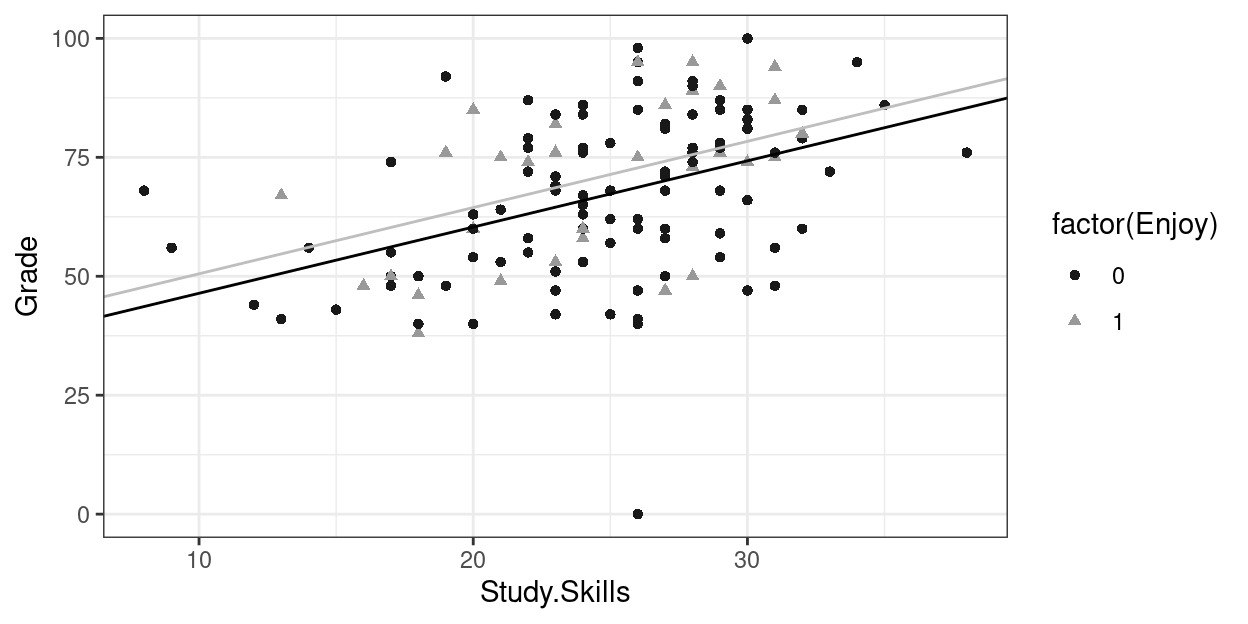
\includegraphics{_main_files/figure-latex/unnamed-chunk-87-1.pdf}

\begin{Shaded}
\begin{Highlighting}[]
\CommentTok{\# plotting the points and lines set up the plot:}
\NormalTok{p1 }\OtherTok{\textless{}{-}} \FunctionTok{ggplot}\NormalTok{(Study\_habits, }\FunctionTok{aes}\NormalTok{(}\AttributeTok{x =}\NormalTok{ Study.Skills, }\AttributeTok{y =}\NormalTok{ Grade, }\AttributeTok{colour =} \FunctionTok{factor}\NormalTok{(Enjoy)))}
\CommentTok{\# size and colour of the points by Enjoy}
\NormalTok{p1 }\OtherTok{\textless{}{-}}\NormalTok{ p1 }\SpecialCharTok{+} \FunctionTok{geom\_point}\NormalTok{(}\FunctionTok{aes}\NormalTok{(}\AttributeTok{shape =} \FunctionTok{factor}\NormalTok{(Enjoy)))}
\CommentTok{\# Note: it\textquotesingle{}s easier in ggplot to plot lines with interactions! Plot the line}
\CommentTok{\# with intercept and slope only for Enjoy=0}
\NormalTok{p1 }\OtherTok{\textless{}{-}}\NormalTok{ p1 }\SpecialCharTok{+} \FunctionTok{geom\_abline}\NormalTok{(}\AttributeTok{intercept =} \FunctionTok{coef}\NormalTok{(grade.lm}\FloatTok{.1}\NormalTok{)[}\DecValTok{1}\NormalTok{], }\AttributeTok{slope =} \FunctionTok{coef}\NormalTok{(grade.lm}\FloatTok{.1}\NormalTok{)[}\DecValTok{2}\NormalTok{],}
    \AttributeTok{color =} \StringTok{"black"}\NormalTok{)}
\CommentTok{\# Plot the line with intercept = intercept+coefficient of Enjoy and slope for}
\CommentTok{\# Enjoy=1}
\NormalTok{p1 }\OtherTok{\textless{}{-}}\NormalTok{ p1 }\SpecialCharTok{+} \FunctionTok{geom\_abline}\NormalTok{(}\AttributeTok{intercept =}\NormalTok{ (}\FunctionTok{coef}\NormalTok{(grade.lm}\FloatTok{.1}\NormalTok{)[}\DecValTok{1}\NormalTok{] }\SpecialCharTok{+} \FunctionTok{coef}\NormalTok{(grade.lm}\FloatTok{.1}\NormalTok{)[}\DecValTok{3}\NormalTok{]), }\AttributeTok{slope =} \FunctionTok{coef}\NormalTok{(grade.lm}\FloatTok{.1}\NormalTok{)[}\DecValTok{2}\NormalTok{],}
    \AttributeTok{color =} \StringTok{"gray"}\NormalTok{)}
\CommentTok{\# make it black and white (ignore for now but useful for black and white}
\CommentTok{\# printing)}
\NormalTok{p1 }\OtherTok{\textless{}{-}}\NormalTok{ p1 }\SpecialCharTok{+} \FunctionTok{scale\_colour\_grey}\NormalTok{(}\AttributeTok{start =} \FloatTok{0.1}\NormalTok{, }\AttributeTok{end =} \FloatTok{0.6}\NormalTok{) }\SpecialCharTok{+} \FunctionTok{theme\_bw}\NormalTok{()}
\NormalTok{p1}
\end{Highlighting}
\end{Shaded}

\fcolorbox{black}{white}{\color{black}
\begin{minipage}[c][16.5cm][t]{\textwidth}
\sffamily\fboxrule.1em\fboxsep1em
Use this section to write notes to help you understand the code.
\end{minipage}}

As we saw in the lectures, when we don't include an interaction between \texttt{Enjoy} and \texttt{Study.Skills} the lines are parallel. This is because the line is using \texttt{Enjoy} to change the intercept only. The regression looks like this:

\[ E(Grade) =32.51 + 1.39 Study.Skills + 4.1 Enjoy \]
So, when \texttt{Enjoy}=0 the line is:
\[ E(Grade) =32.51 + 1.39 Study.Skills\]
But when \texttt{Enjoy}=1 the line is
\[ E(Grade)  =32.51 + 1.39 Study.Skills + 4.1\]
\[ = 36.61 + 1.39 Study.Skills\]

\hypertarget{interpreting-coefficients}{%
\subsubsection{Interpreting coefficients}\label{interpreting-coefficients}}

\begin{itemize}
\tightlist
\item
  The \emph{intercept}: A students with no study skills (\texttt{Study.Skills}=0) and who does not enjoy statistics (\texttt{Enjoy}=0) has a predicted Grade of 32.51. Again not very useful as \texttt{Study.Skills}=0 is unlikely.
\item
  The \emph{coefficient} of \texttt{Enjoy}: When we look at students who have \emph{the same} level of \texttt{Study.Skills} then those who Enjoy statistics are on average getting 4.1 more in their Grade than those who do not Enjoy.
\item
  The \emph{coefficient} of \texttt{Study.Skills}: When we look at students who enjoy statistics we expect them to get on average 1.39 more in their grade for every additional point in study skills score. Same for students who do not enjoy statistics.
\end{itemize}

The basic idea behind interpreting coefficients is thinking how changing one predictor changes the average outcome \emph{while keeping everthing else the} \textbf{same}.

\hypertarget{subset-regression}{%
\subsection{Subset regression}\label{subset-regression}}

Let's divide the data into two groups, those who enjoy statistics and those who don't and run separate regressions.

First we create two new subsets:

\begin{Shaded}
\begin{Highlighting}[]
\CommentTok{\#Subset the data and then run the regression of Grade on Study.Skills for each subset}
\NormalTok{Study\_habits.Enj1}\OtherTok{\textless{}{-}}\FunctionTok{subset}\NormalTok{(Study\_habits, Enjoy}\SpecialCharTok{==}\DecValTok{1}\NormalTok{)}
\NormalTok{lm.Enj1}\OtherTok{\textless{}{-}}\FunctionTok{lm}\NormalTok{(Grade}\SpecialCharTok{\textasciitilde{}}\NormalTok{Study.Skills,}\AttributeTok{data=}\NormalTok{Study\_habits.Enj1)}
\NormalTok{Study\_habits.Enj0}\OtherTok{\textless{}{-}}\FunctionTok{subset}\NormalTok{(Study\_habits, Enjoy}\SpecialCharTok{==}\DecValTok{0}\NormalTok{)}
\NormalTok{lm.Enj0}\OtherTok{\textless{}{-}}\FunctionTok{lm}\NormalTok{(Grade}\SpecialCharTok{\textasciitilde{}}\NormalTok{Study.Skills,}\AttributeTok{data=}\NormalTok{Study\_habits.Enj0)}
\end{Highlighting}
\end{Shaded}

Then create two separate slopes on the same plot:

\begin{Shaded}
\begin{Highlighting}[]
\CommentTok{\# Basic plot p1 of Grade against Study.Skills distingushing points by Enjoy}
\NormalTok{p1 }\OtherTok{\textless{}{-}} \FunctionTok{ggplot}\NormalTok{(Study\_habits, }\FunctionTok{aes}\NormalTok{(}\AttributeTok{x =}\NormalTok{ Study.Skills, }\AttributeTok{y =}\NormalTok{ Grade, }\AttributeTok{colour =} \FunctionTok{factor}\NormalTok{(Enjoy)))}
\NormalTok{p1 }\OtherTok{\textless{}{-}}\NormalTok{ p1 }\SpecialCharTok{+} \FunctionTok{geom\_point}\NormalTok{(}\FunctionTok{aes}\NormalTok{(}\AttributeTok{shape =} \FunctionTok{factor}\NormalTok{(Enjoy)))}
\CommentTok{\# Plot a line based on the lm.Int0 for the subset of people with Enjoy=0}
\NormalTok{p1 }\OtherTok{\textless{}{-}}\NormalTok{ p1 }\SpecialCharTok{+} \FunctionTok{geom\_abline}\NormalTok{(}\AttributeTok{intercept =} \FunctionTok{coef}\NormalTok{(lm.Enj0)[}\DecValTok{1}\NormalTok{], }\AttributeTok{slope =} \FunctionTok{coef}\NormalTok{(lm.Enj0)[}\DecValTok{2}\NormalTok{], }\AttributeTok{color =} \StringTok{"black"}\NormalTok{)}
\CommentTok{\# Plot a line based on the lm.Int1 for the subset of people with Enjoy=1}
\NormalTok{p1 }\OtherTok{\textless{}{-}}\NormalTok{ p1 }\SpecialCharTok{+} \FunctionTok{geom\_abline}\NormalTok{(}\AttributeTok{intercept =} \FunctionTok{coef}\NormalTok{(lm.Enj1)[}\DecValTok{1}\NormalTok{], }\AttributeTok{slope =} \FunctionTok{coef}\NormalTok{(lm.Enj1)[}\DecValTok{2}\NormalTok{], }\AttributeTok{color =} \StringTok{"gray"}\NormalTok{)}
\CommentTok{\# for black and white. you can ignore}
\NormalTok{p1 }\OtherTok{\textless{}{-}}\NormalTok{ p1 }\SpecialCharTok{+} \FunctionTok{scale\_colour\_grey}\NormalTok{(}\AttributeTok{start =} \FloatTok{0.1}\NormalTok{, }\AttributeTok{end =} \FloatTok{0.6}\NormalTok{) }\SpecialCharTok{+} \FunctionTok{theme\_bw}\NormalTok{()}
\NormalTok{p1}
\end{Highlighting}
\end{Shaded}

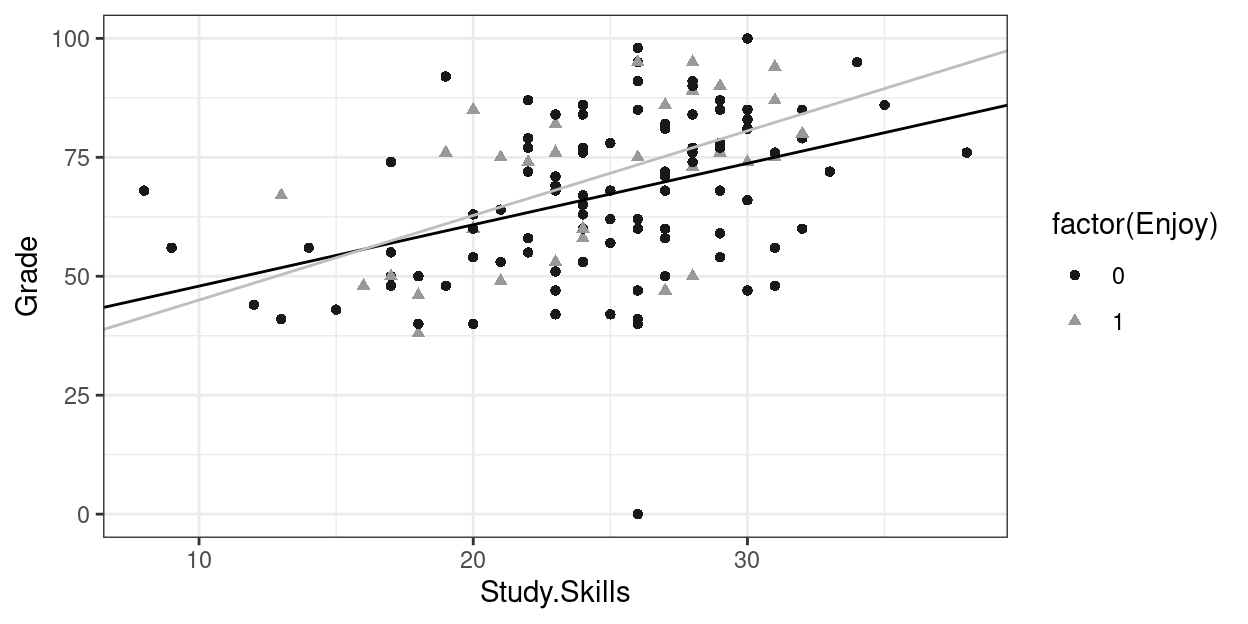
\includegraphics{_main_files/figure-latex/unnamed-chunk-90-1.pdf}

\hypertarget{interactions}{%
\subsection{Interactions}\label{interactions}}

From the scatterplot above and from the regression, the effect of \texttt{Enjoy} does not appear to be very strong, however there is no way of knowing this for sure until we look at the formal diagnostics later. So let's try adding an interaction.

\begin{Shaded}
\begin{Highlighting}[]
\NormalTok{grade.enjoy.lm.int}\OtherTok{\textless{}{-}}\FunctionTok{lm}\NormalTok{(Grade}\SpecialCharTok{\textasciitilde{}}\NormalTok{Study.Skills}\SpecialCharTok{*}\NormalTok{Enjoy,}\AttributeTok{data=}\NormalTok{Study\_habits)}
\FunctionTok{display}\NormalTok{(grade.enjoy.lm.int)}
\end{Highlighting}
\end{Shaded}

\begin{verbatim}
## lm(formula = Grade ~ Study.Skills * Enjoy, data = Study_habits)
##                    coef.est coef.se
## (Intercept)        35.04     7.29  
## Study.Skills        1.29     0.29  
## Enjoy              -7.81    15.67  
## Study.Skills:Enjoy  0.49     0.63  
## ---
## n = 134, k = 4
## residual sd = 15.54, R-Squared = 0.19
\end{verbatim}

\fcolorbox{black}{white}{\color{black}
\begin{minipage}[c][6cm][t]{\textwidth}
\sffamily\fboxrule.1em\fboxsep1em
Q: Write down two regressions, one for the case where \texttt{Enjoy} is 0 and another for \texttt{Enjoy} is 1.

\end{minipage}}

\newpage

The code for interactions in the \texttt{ggplot()} it much easier as you can see:

\begin{Shaded}
\begin{Highlighting}[]
\CommentTok{\#Basic plot}
\NormalTok{p1}\OtherTok{\textless{}{-}}\FunctionTok{ggplot}\NormalTok{(Study\_habits, }\FunctionTok{aes}\NormalTok{(}\AttributeTok{x=}\NormalTok{Study.Skills, }\AttributeTok{y=}\NormalTok{Grade,}\AttributeTok{colour=}\FunctionTok{factor}\NormalTok{(Enjoy)))}
\CommentTok{\#add points}
\NormalTok{p1}\OtherTok{\textless{}{-}}\NormalTok{ p1 }\SpecialCharTok{+} \FunctionTok{geom\_point}\NormalTok{(}\FunctionTok{aes}\NormalTok{(}\AttributeTok{shape=}\FunctionTok{factor}\NormalTok{(Enjoy)))}
\CommentTok{\#In ggplot it is much easier to plot the interaction!}
\CommentTok{\# se=FALSE doesn\textquotesingle{}t add the standard error range to the regression. Try without it!}
\NormalTok{p1}\OtherTok{\textless{}{-}}\NormalTok{ p1}\SpecialCharTok{+}\FunctionTok{geom\_smooth}\NormalTok{(}\AttributeTok{method=}\StringTok{"lm"}\NormalTok{, }\AttributeTok{se=}\ConstantTok{FALSE}\NormalTok{) }
\CommentTok{\#black and white colour scheme, you can ignore}
\NormalTok{p1}\OtherTok{\textless{}{-}}\NormalTok{ p1 }\SpecialCharTok{+}\FunctionTok{scale\_colour\_grey}\NormalTok{(}\AttributeTok{start =} \FloatTok{0.1}\NormalTok{, }\AttributeTok{end =} \FloatTok{0.6}\NormalTok{)  }\SpecialCharTok{+} \FunctionTok{theme\_bw}\NormalTok{()}
\NormalTok{p1}
\end{Highlighting}
\end{Shaded}

\begin{verbatim}
## `geom_smooth()` using formula 'y ~ x'
\end{verbatim}

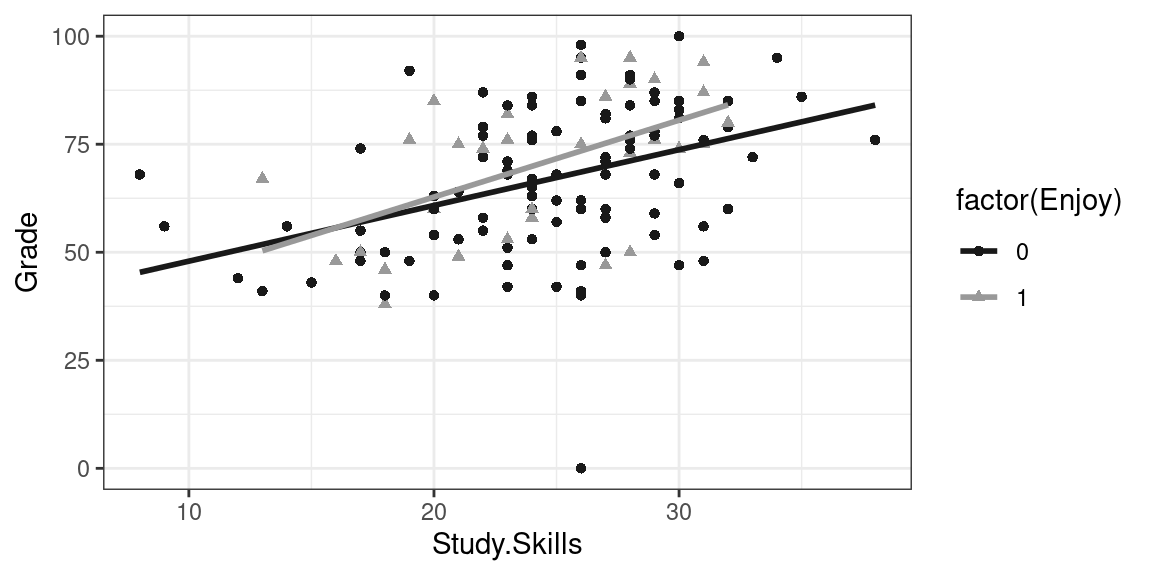
\includegraphics{_main_files/figure-latex/unnamed-chunk-92-1.pdf}

\fcolorbox{black}{white}{\color{black}
\begin{minipage}[c][6cm][t]{\textwidth}
\sffamily\fboxrule.1em\fboxsep1em
Q: Based on the plot and the output from the regression, do you think \texttt{Enjoy} makes a difference to the average \texttt{Grade}? Does it interact with \texttt{Study.Skills}? Justify your answer.

\end{minipage}}

\newpage

\hypertarget{diagnostics-part-2}{%
\subsection{Diagnostics Part 2}\label{diagnostics-part-2}}

Diagnostic statistics are used to assess how well a model fits the data. They are useful tool for model comparison and fitting, however they should \textbf{never} be the only way you assess a model or make decisions about whether to keep a variable in a regression or not. Over the course of this term I will teach you other important approaches.

\emph{A QUICK GUIDE TO MODEL ASSESSMENT} can be found at the back of the book. This will be useful for the Reading week project and is the \emph{minimum} you need to do in any analysis.

Remember that there are \emph{five} main diagnostics. We're familiar with some of them:

\begin{enumerate}
\def\labelenumi{\arabic{enumi}.}
\tightlist
\item
  The standard deviation of the regression line -- also known as the \emph{residual standard error}
\item
  The R\(^2\) (\texttt{R-squared/Multiple\ R-squared}) and
\item
  The Adjusted R\(^2\) (\texttt{Adjusted\ R-squared})
\item
  The significance at the 5\% level of the p-value of the t-statistics of the regression coefficients
\item
  The significance at the 5\% level of the p-value of F-statistic of the regression
\end{enumerate}

From \texttt{display()} we can get the \(R^2\), the residual standard error and we can calculate the approximate 95\% confidence interval which in turn tells us whether the coefficients are significant at the 5\% level. Let's add all the predictors we have considered to be important to the regression. We also remove the Grade=0 point.

\begin{Shaded}
\begin{Highlighting}[]
\NormalTok{Study\_Habits}\OtherTok{\textless{}{-}}\FunctionTok{read.csv}\NormalTok{(}\StringTok{"../Data/Stats\_study\_habits\_noout.csv"}\NormalTok{,}\AttributeTok{header=}\NormalTok{T)}
\NormalTok{grade.lm}\OtherTok{\textless{}{-}}\FunctionTok{lm}\NormalTok{(Grade}\SpecialCharTok{\textasciitilde{}}\NormalTok{Study.Skills}\SpecialCharTok{+}\NormalTok{Interesting}\SpecialCharTok{+}\NormalTok{Enjoy,}\AttributeTok{data=}\NormalTok{Study\_Habits)}
\FunctionTok{display}\NormalTok{(grade.lm)}
\end{Highlighting}
\end{Shaded}

\begin{verbatim}
## lm(formula = Grade ~ Study.Skills + Interesting + Enjoy, data = Study_Habits)
##              coef.est coef.se
## (Intercept)  24.24     7.48  
## Study.Skills  1.41     0.32  
## Interesting  10.10     3.52  
## Enjoy         3.25     3.43  
## ---
## n = 85, k = 4
## residual sd = 13.80, R-Squared = 0.35
\end{verbatim}

We cannot calculate the F-statistic or the Adjusted R\(^2\) from this. In order to get all these values we use \texttt{summary()}

\begin{Shaded}
\begin{Highlighting}[]
\FunctionTok{summary}\NormalTok{(grade.lm)}
\end{Highlighting}
\end{Shaded}

\begin{verbatim}
## 
## Call:
## lm(formula = Grade ~ Study.Skills + Interesting + Enjoy, data = Study_Habits)
## 
## Residuals:
##      Min       1Q   Median       3Q      Max 
## -29.9641  -8.7788  -0.7915  10.2085  27.3938 
## 
## Coefficients:
##              Estimate Std. Error t value Pr(>|t|)    
## (Intercept)   24.2370     7.4787   3.241  0.00173 ** 
## Study.Skills   1.4074     0.3154   4.462 2.59e-05 ***
## Interesting   10.0990     3.5246   2.865  0.00531 ** 
## Enjoy          3.2500     3.4320   0.947  0.34647    
## ---
## Signif. codes:  0 '***' 0.001 '**' 0.01 '*' 0.05 '.' 0.1 ' ' 1
## 
## Residual standard error: 13.8 on 81 degrees of freedom
## Multiple R-squared:  0.352,  Adjusted R-squared:  0.328 
## F-statistic: 14.67 on 3 and 81 DF,  p-value: 1.026e-07
\end{verbatim}

\#\#\#F-statistic

The F-statistic is a measure of how good the model \emph{as a whole} is. We are usually interested in the p-value associated with it. Let us consider a regression given by:

\(y_i = \beta_0+ \beta_1 x_{1i} + \beta_2 x_{2i} + \ldots \beta_p x_{pi}\)

Then, for the F-test,

\begin{itemize}
\tightlist
\item
  The \emph{null hypothesis} , \(H_0: \,\, \beta_1=\beta_2= \ldots =\beta_p=0\)
\item
  The \emph{alternative hypothesis} \(H_1:\) is \emph{at least one} of \(\beta_1,\beta_2, \ldots ,\beta_p\) \emph{is not} equal to 0.
\end{itemize}

The F-test tells us whether there is at least one predictor that explains some of the outcome. It doesn't say which are the important ones. When there is a problem of \emph{multicollinearity} (more later) it can be useful because the F-statistic may well be significant at the 5\% level while all the predictors are not.

\fcolorbox{black}{white}{\color{black}
\begin{minipage}[c][3cm][t]{\textwidth}
\sffamily\fboxrule.1em\fboxsep1em
Q: Based on the output of \texttt{summary()} above, is the F-statistic significant at the 5\% level? What does this imply for the model as a whole?

\end{minipage}}

The F-test is a special case of the \emph{partial F-test}. The partial F-test can be used to assess the joint significance of a group of predictors. Let us again consider a regression given by:

\(y_i = \beta_0+ \beta_1 x_{1i} + \beta_2 x_{2i} + \ldots \beta_p x_{pi}\)

Let's say we want to add the following predictors: \(x_{p+1},\ldots,x_q\) where \(q > p\) to the model. We may then run the following test:

\begin{itemize}
\tightlist
\item
  The \emph{null hypothesis}, \(H_0: \,\, \beta_{p+1}=\beta_{p+2}= \ldots =\beta_q=0\)
\item
  The \emph{alternative hypothesis}, \(H_1:\) is \emph{at least one} of \(\beta_{p+1},\beta_{p+2}, \ldots ,\beta_q\) \emph{is not} equal to 0.
\end{itemize}

We are therefore asking whether the subset \(x_{p+1},\ldots,x_q\) of predictors are significant as a whole and adding them improves the regression model.

\hypertarget{adjusted-r2}{%
\subsubsection{\texorpdfstring{Adjusted R\(^2\)}{Adjusted R\^{}2}}\label{adjusted-r2}}

The Adjusted R\(^2\) is designed to be interpreted in the same way as the R\(^2\) but for multiple rather than simple linear regression. It takes into account the loss of information incurred by adding a non-significant variable. In practice if a variable is non-significant this can be deduced from the 95\% confidence interval. There are two rules of thumb with using the Adjusted R\(^2\) as a measure of model fit. For a good model:

\begin{enumerate}
\def\labelenumi{\arabic{enumi}.}
\tightlist
\item
  It should be within 4\% of the R\(^2\) -- otherwise there are probably too many non-significant predictors in the model
\item
  It should be close to 1 -- same as the R\(^2\).
\end{enumerate}

\fcolorbox{black}{white}{\color{black}
\begin{minipage}[c][3.5cm][t]{\textwidth}
\sffamily\fboxrule.1em\fboxsep1em
Write down the formula for the Adjusted R$^2$:

\end{minipage}}

\hypertarget{ifelse}{%
\subsubsection{\texorpdfstring{\texttt{ifelse()}}{ifelse()}}\label{ifelse}}

\texttt{ifelse()} is a function that is necessary if using the \texttt{plot()} command to visualise the effect of adding a categorical variable to a regression. However it has other uses and is worth understanding. It is a one line function that works as follows:

\texttt{ifelse(A,IF\ A=TRUE\ DO\ THIS,\ ELSE\ (i.e.\ A=FALSE)\ DO\ THIS)}

There is also a longer version which has the \texttt{if} and the \texttt{else} separated and should be used when the commands for if and else are long and complex.

An easy example is of \texttt{ifelse()} is:

\begin{Shaded}
\begin{Highlighting}[]
\NormalTok{x}\OtherTok{\textless{}{-}}\DecValTok{1}
\FunctionTok{ifelse}\NormalTok{(x}\SpecialCharTok{\textgreater{}}\DecValTok{0}\NormalTok{,}\StringTok{"hello"}\NormalTok{,}\StringTok{"bye"}\NormalTok{)}
\end{Highlighting}
\end{Shaded}

\begin{verbatim}
## [1] "hello"
\end{verbatim}

\begin{Shaded}
\begin{Highlighting}[]
\NormalTok{x}\OtherTok{\textless{}{-}} \SpecialCharTok{{-}}\DecValTok{1}
\FunctionTok{ifelse}\NormalTok{(x}\SpecialCharTok{\textgreater{}}\DecValTok{0}\NormalTok{,}\StringTok{"hello"}\NormalTok{,}\StringTok{"bye"}\NormalTok{)}
\end{Highlighting}
\end{Shaded}

\begin{verbatim}
## [1] "bye"
\end{verbatim}

The long version is

\begin{Shaded}
\begin{Highlighting}[]
\ControlFlowTok{if}\NormalTok{(x}\SpecialCharTok{\textgreater{}}\DecValTok{0}\NormalTok{)}
\NormalTok{\{}
  \StringTok{"hello"}
\NormalTok{\} }\ControlFlowTok{else}\NormalTok{ \{}
  \StringTok{"bye"}
\NormalTok{\}}
\end{Highlighting}
\end{Shaded}

\begin{verbatim}
## [1] "bye"
\end{verbatim}

\hypertarget{lecture-5-multiple-linear-regression-part-2}{%
\section{Lecture 5: Multiple Linear Regression part 2}\label{lecture-5-multiple-linear-regression-part-2}}

\hypertarget{learning-outcomes-7}{%
\subsection{Learning Outcomes}\label{learning-outcomes-7}}

Understanding Categorical variables

Using the partial F-statistic and \texttt{Anova()} in the ``car'' package to assess the significance of a categorical variable in linear regression

Understanding the concepts of overfitting and multicollinearity

\hypertarget{data-3}{%
\subsection{Data}\label{data-3}}

In this session we'll use the Study Skills data set. We'll initially include the categorical variable \texttt{Social.Net} and later the predictor \texttt{A.Level}. \texttt{A.Level} in principle has a range from 0-6, however in our data we only see the values 4,5 and 6 and only one person has a 4. As a consequence although it could be considered a continuous variable, we treat it as a categorical variable.

\begin{longtable}[]{@{}
  >{\centering\arraybackslash}p{(\columnwidth - 4\tabcolsep) * \real{0.1259}}
  >{\centering\arraybackslash}p{(\columnwidth - 4\tabcolsep) * \real{0.0963}}
  >{\raggedright\arraybackslash}p{(\columnwidth - 4\tabcolsep) * \real{0.7778}}@{}}
\toprule()
\begin{minipage}[b]{\linewidth}\centering
Name
\end{minipage} & \begin{minipage}[b]{\linewidth}\centering
Type
\end{minipage} & \begin{minipage}[b]{\linewidth}\raggedright
Description
\end{minipage} \\
\midrule()
\endhead
Study Skills & continuous & 0-56 Total study skills - higher is more skills \\
Grade & continuous & grades in stats exam out of 100 \\
Social.Net & categorical & 1 - less than 1 hour a week,2-between 1 and 4 hours,3-over 4 hours \\
A.Level & categorical & 4,5,6 the grade received at A-level for mathematics or statistics. \\
\bottomrule()
\end{longtable}

\begin{Shaded}
\begin{Highlighting}[]
\NormalTok{Study\_habits}\OtherTok{\textless{}{-}}\FunctionTok{read.csv}\NormalTok{(}\StringTok{"../Data/Stats\_study\_habits\_noout.csv"}\NormalTok{)}
\end{Highlighting}
\end{Shaded}

\hypertarget{social.net}{%
\subsubsection{\texorpdfstring{\texttt{Social.Net}}{Social.Net}}\label{social.net}}

\texttt{Social.Net} tells us how many hours students spend on social networks in a week. It is coded in the data as 1,2,3 representing less than one hour of social networking a week, between 1 and 4 hours and more than 4 hours a week respectively.

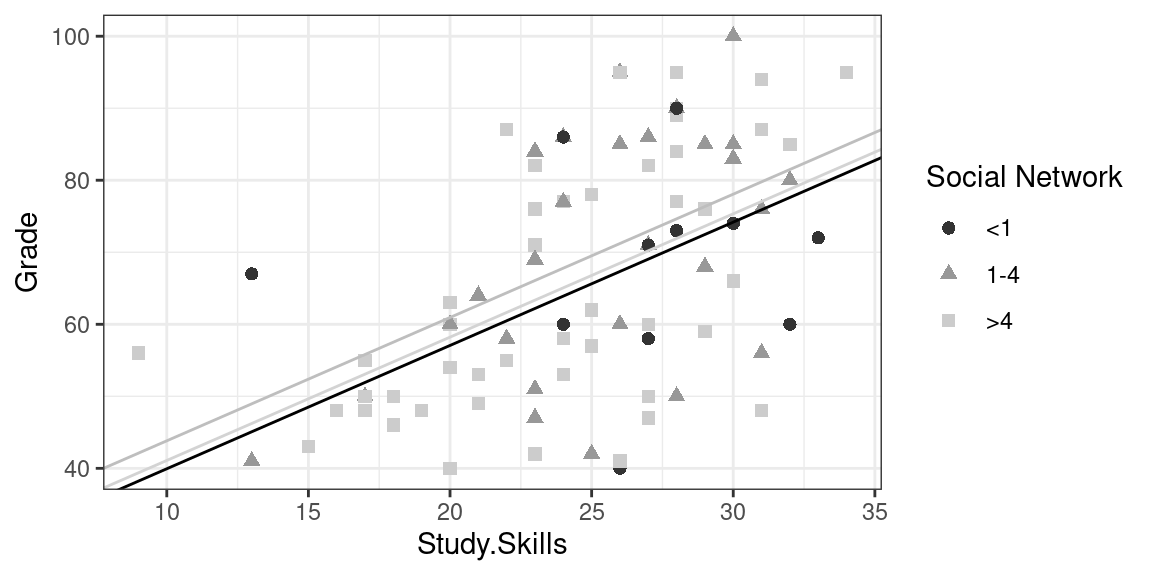
\includegraphics{_main_files/figure-latex/unnamed-chunk-98-1.pdf}

\fcolorbox{black}{white}{\color{black}
\begin{minipage}[c][4.5cm][t]{\textwidth}
\sffamily\fboxrule.1em\fboxsep1em
Q: Based on the boxplot do you think that ``Social.Net`` has an impact on Grade? Why?

\end{minipage}}

\hypertarget{categorical-variables}{%
\subsection{Categorical variables}\label{categorical-variables}}

A variable is categorical when a variable has \emph{discrete values} such that the \emph{difference} between one value and another is not the same across variables. Ordinal variables are categorical variables with an inherent ordering (e.g.~age or income bands)

\textbf{Exercise}

\fcolorbox{black}{white}{\color{black}
\begin{minipage}[c][4.5cm][t]{\textwidth}
\sffamily\fboxrule.1em\fboxsep1em
Q: Give an example of a variable with discrete values that is \textbf{not} categorical
\\
\\
\\
Q: Give an example of a variable with discrete values that \textbf{is} categorical


\end{minipage}}

Categorical variables behave the same way as binary variables except they have more levels. Consider adding \texttt{Social.Net} to the regression with \texttt{Study.Skills}. Like the binary variable \texttt{Interesting}, \texttt{Social.Net} results in multiple lines, one for each level of the variable.

Binary variables have 2 levels and are included as a single predictor in the regression. There is one line when the value of the binary variable =0 (or the \emph{baseline} , e.g.~``Female'') and another one for when the binary variable=1 (or the other value, e.g.~``Male''). For categorical variables with k levels there are k lines and they are included in the regression as \textbf{k-1} predictor variables. These predictors are binary and they are called \emph{dummy} variables.

\texttt{Social.Net} has 3 levels coded as 1, 2, 3 corresponding to (\textless1,1-4,\textgreater4) indicating the number hours per week spent on social networks. So we define 2 new binary dummy variables:

\[
    \text{f.Social.Net14}= 
\begin{cases}
    1 & \text{if Social.Net="1-4"}\\
    0,              & \text{otherwise}
\end{cases}
\]
and
\[
    \text{f.Social.Net4}= 
\begin{cases}
    1 & \text{if Social.Net=">4"}\\
    0,              & \text{otherwise}
\end{cases}
\]
This means that when \texttt{f.Social.Net14=f.Social.Net4}=0 then\texttt{Social.Net}=\textless1. We then term \texttt{Social.Net}=``\textless1'' the \emph{baseline}.

\color{white} zzzzzz \color{black} \fcolorbox{black}{lightgray!20!white}{\color{black}
\begin{minipage}[c][4cm][t]{12.5cm}
\textbf{Dummy variables and baseline/reference levels}: When we include a categorical variable with k levels in a regression we do two things:
\begin{enumerate}
\item First we choose a baseline/reference level. The baseline level of the categorical variable is the one that corresponds to 0 values for all the other levels. It is also that the others will be compared with. Often this is the most commonly occurring or the one of most interest.
\item Second we create k-1 binary dummies, one for each of the non-baseline levels. For a data point with level j (where j is between 1 and k-1), the dummies will all have 0 value except for the one corresponding to level j.
\end{enumerate}
\end{minipage}}

Formally in the model without interactions:
\[Grade=\beta_0 + \beta_1 Study.Skills + \beta_2 f.Social.Net14 +  \beta_3 f.Social.Net4\]
This results in the following 3 lines:

\texttt{Social.Net}=1, (``\textless1''):
\[Grade=\beta_0 + \beta_1 Study.Skills\]
\texttt{Social.Net}=2, (``1-4'')
\[Grade=(\beta_0+\beta_2) + \beta_1 Study.Skills\]
\texttt{Social.Net}=3, (``\textgreater4''):
\[Grade=(\beta_0+\beta_3) + \beta_1 Study.Skills\]

We can see from the formulae above that the coefficient of \texttt{f.Social.Net14}, \(\beta_2\) is the average difference in Grade between students who spend less than 1 hour on social networks and those who spend between 1 and 4 hours on social networks per week.

\fcolorbox{black}{white}{\color{black}
\begin{minipage}[c][4.5cm][t]{\textwidth}
\sffamily\fboxrule.1em\fboxsep1em
Q: What does the value of $\beta_3$ correspond to?\\
\\
\\
\\
Q: How would you calculate the average difference in Grade for students spending between 1 and 4 and those spending more than 4 hours per week on social networks?


\end{minipage}}

Let's run a regression. Notice that we have to tell \texttt{R} that \texttt{Social.Net} is a categorical variable by adding \texttt{as.factor()} or \texttt{factor()}.

\color{white} zzzzzz \color{black} \fcolorbox{black}{lightgray!20!white}{\color{black}
\begin{minipage}[c][4.5cm][t]{12.5cm}
Adding categorical predictors to regressions in \texttt{R}. 
\begin{enumerate}
\item When you add a categorical predictor to \texttt{R} you do not need to add each of the dummy variables as \texttt{R} recognises that the predictor is categorical and automatically creates the dummies. Bear in mind that if you do not set the reference level then \texttt{R} will choose the first in alphabetical/numeric order as the reference level. I'll show you later how to set the reference level.
\item \texttt{factor()}: When a predictor is categorical and coded in the data set as an integer value then you must include it in a regression as \texttt{factor(x)} as otherwise \texttt{R} will not recognise it as a categorical variable and create dummies. It is not necessary when the variable is coded as text.
\end{enumerate}
\end{minipage}}

\begin{Shaded}
\begin{Highlighting}[]
\NormalTok{grade.lm}\FloatTok{.1}\OtherTok{\textless{}{-}}\FunctionTok{lm}\NormalTok{(Grade}\SpecialCharTok{\textasciitilde{}}\NormalTok{Study.Skills}\SpecialCharTok{+}\FunctionTok{factor}\NormalTok{(Social.Net),}\AttributeTok{data=}\NormalTok{Study\_habits)}
\FunctionTok{display}\NormalTok{(grade.lm}\FloatTok{.1}\NormalTok{)}
\end{Highlighting}
\end{Shaded}

\begin{verbatim}
## lm(formula = Grade ~ Study.Skills + factor(Social.Net), data = Study_habits)
##                     coef.est coef.se
## (Intercept)         22.82     9.51  
## Study.Skills         1.71     0.32  
## factor(Social.Net)2  3.88     5.21  
## factor(Social.Net)3  1.16     4.95  
## ---
## n = 85, k = 4
## residual sd = 14.53, R-Squared = 0.28
\end{verbatim}

\begin{center}\includegraphics{_main_files/figure-latex/unnamed-chunk-100-1} \end{center}

\fcolorbox{black}{white}{\color{black}
\begin{minipage}[c][7cm][t]{\textwidth}
\sffamily\fboxrule.1em\fboxsep1em
Q: Write down the regression lines for the 3 different levels of ``Social.Net``


\end{minipage}}

Note that the lines are very close to one another meaning that the difference between the baseline and the other categories is not large. This fits with the coefficients for the \texttt{Social.Net} categories not being significant at the 5\% level.

\hypertarget{adding-an-interaction}{%
\subsection{Adding an interaction}\label{adding-an-interaction}}

If we add a \texttt{Study.Skills} and \texttt{Social.Net} interaction what does the regression look like?

\begin{verbatim}
## `geom_smooth()` using formula 'y ~ x'
## `geom_smooth()` using formula 'y ~ x'
\end{verbatim}

\includegraphics{_main_files/figure-latex/unnamed-chunk-101-1.pdf}

The regression output is:

\begin{verbatim}
## lm(formula = Grade ~ Study.Skills * factor(Social.Net), data = Study_habits)
##                                  coef.est coef.se
## (Intercept)                       64.32    23.00 
## Study.Skills                       0.15     0.85 
## factor(Social.Net)2              -46.07    28.12 
## factor(Social.Net)3              -45.37    24.99 
## Study.Skills:factor(Social.Net)2   1.90     1.06 
## Study.Skills:factor(Social.Net)3   1.78     0.94 
## ---
## n = 85, k = 6
## residual sd = 14.36, R-Squared = 0.32
\end{verbatim}

\fcolorbox{black}{white}{\color{black}
\begin{minipage}[c][7cm][t]{\textwidth}
\sffamily\fboxrule.1em\fboxsep1em
Q: Write down the regression lines for the 3 different levels of ``Social.Net``


\end{minipage}}

The interaction made a \emph{big} difference! None of the predictors are significant any more! To see this, compare the output above to that of \texttt{grade.lm.1}.

There are two reasons.

\begin{enumerate}
\def\labelenumi{\arabic{enumi}.}
\tightlist
\item
  The first is that by allowing the interaction, the line of best fit for those spending less than one hour on social networks per week (black dots in the scatterplot) is driven by the point on the far left.
\item
  The second reason is that the smaller sample size means that there is insufficient \emph{power} to estimate the 6 parameters with more certainty -- i.e.~with confidence intervals that do not include 0.
\end{enumerate}

We can however do subset regression:

\begin{verbatim}
## # A tibble: 6 x 6
## # Groups:   Social.Net [3]
##   Social.Net term         estimate std.error statistic   p.value
##        <int> <chr>           <dbl>     <dbl>     <dbl>     <dbl>
## 1          1 (Intercept)    64.3      23.3       2.76  0.0220   
## 2          1 Study.Skills    0.149     0.861     0.173 0.867    
## 3          3 (Intercept)    19.0       9.63      1.97  0.0553   
## 4          3 Study.Skills    1.92      0.396     4.85  0.0000150
## 5          2 (Intercept)    18.2      16.5       1.11  0.279    
## 6          2 Study.Skills    2.04      0.638     3.21  0.00367
\end{verbatim}

The table above shows in the firs column the value of \texttt{Social.Net} for this subset regression. So the first two rows correspond to the subset of students with \texttt{Social.Net=1}. The second column indicates whether the parameter is the intercept of the slope of \texttt{Study.Skills}. The remaining columns are the value of the estimate, its standard error, the value of the t-statistic and the corresponding p-value. We can also use the \texttt{facet\_wrap()} function for \texttt{ggplot()}.

\texttt{facet\_wrap()} is a convenient way of showing the effect of interactions by only looking at the points involved in each interaction.

\begin{Shaded}
\begin{Highlighting}[]
\NormalTok{p1 }\OtherTok{\textless{}{-}} \FunctionTok{ggplot}\NormalTok{(}\AttributeTok{data =}\NormalTok{ Study\_habits, }\FunctionTok{aes}\NormalTok{(}\AttributeTok{x =}\NormalTok{ Study.Skills, }\AttributeTok{y =}\NormalTok{ Grade))}
\NormalTok{p1 }\OtherTok{\textless{}{-}}\NormalTok{ p1 }\SpecialCharTok{+} \FunctionTok{geom\_point}\NormalTok{(}\AttributeTok{size =} \FloatTok{0.5}\NormalTok{) }\SpecialCharTok{+} \FunctionTok{labs}\NormalTok{(}\AttributeTok{title =} \StringTok{"Multiple plots for categorical variables"}\NormalTok{)}
\NormalTok{p1 }\OtherTok{\textless{}{-}}\NormalTok{ p1 }\SpecialCharTok{+} \FunctionTok{facet\_wrap}\NormalTok{(}\SpecialCharTok{\textasciitilde{}}\FunctionTok{factor}\NormalTok{(Social.Net)) }\SpecialCharTok{+} \FunctionTok{geom\_smooth}\NormalTok{(}\AttributeTok{method =} \StringTok{"lm"}\NormalTok{)}
\NormalTok{p1}
\end{Highlighting}
\end{Shaded}

\begin{verbatim}
## `geom_smooth()` using formula 'y ~ x'
\end{verbatim}

\includegraphics{_main_files/figure-latex/unnamed-chunk-105-1.pdf}

\fcolorbox{black}{white}{\color{black}
\begin{minipage}[c][3cm][t]{\textwidth}
\sffamily\fboxrule.1em\fboxsep1em
Q: Based on the output of the subset regression and the plot, which of the slopes are significant at the 5% level? Confirm that the lines are the same as those in the interaction model

\end{minipage}}

\hypertarget{the-partial-f-statistic-and-anova}{%
\subsection{The partial F-statistic and ANOVA()}\label{the-partial-f-statistic-and-anova}}

The \emph{partial} F-statistic is useful when looking at the significance of categorical predictors in a regression as it asks whether a group of predictors are significant. Specifically, in order to understand whether a categorical variable as a whole is significant we run Analysis of Variance (ANOVA) which essentially runs F-tests. This asks whether the means of the outcome is different in different levels of the categorical predictor. Contrast this to the t-tests for the coefficients of categorical dummy variables in linear regression which ask whether the mean outcome in each level is different from the mean outcome in the baseline level.

\#\#Assessing the overall significance of a categorical variable

Let's turn to our Study habits data and include \texttt{A.Level} (as a categorical variable) as well as \texttt{Social.Net} and \texttt{Interesting} which is binary.

\begin{verbatim}
## # A tibble: 3 x 3
##   A.Level Mean.Grade  Size
##     <int>      <dbl> <int>
## 1       4       42       1
## 2       5       67.1    22
## 3       6       67.2    62
\end{verbatim}

The table above shows the value of \texttt{A.Level}, the mean grade in that level of \texttt{A.Level} and the number of students in that group. The regression test whether 67 is significantly different from 42. Even with a sample of 1 for \texttt{A.Level}=4 this comes out as just significant as shown below:

\begin{verbatim}
## lm(formula = Grade ~ Interesting + factor(Social.Net) + factor(A.Level), 
##     data = Study_habits)
##                     coef.est coef.se t value Pr(>|t|)
## (Intercept)         23.44    16.44    1.43    0.16   
## Interesting         15.86     3.63    4.37    0.00   
## factor(Social.Net)2  2.70     5.49    0.49    0.62   
## factor(Social.Net)3 -2.54     5.07   -0.50    0.62   
## factor(A.Level)5    33.96    15.75    2.16    0.03   
## factor(A.Level)6    32.92    15.42    2.13    0.04   
## ---
## n = 85, k = 6
## residual sd = 15.10, R-Squared = 0.24
\end{verbatim}

Rather than comparing whether levels of a categorical predictor as significantly different from one another in the regression a better approach is to try to understand whether the whole categorical variable is significant. We use the F-statistic for sub-groups of coefficients corresponding to the dummy variables associated with the categorical predictor. \emph{Make sure to \emph{capitalize} the A in \texttt{Anova()} or you'll get a different function}. You will also need to load and install the ``car'' package for this \texttt{Anova()} function.

\begin{Shaded}
\begin{Highlighting}[]
\FunctionTok{Anova}\NormalTok{(anova.lm)}
\end{Highlighting}
\end{Shaded}

\begin{verbatim}
## Anova Table (Type II tests)
## 
## Response: Grade
##                     Sum Sq Df F value    Pr(>F)    
## Interesting         4361.6  1 19.1197 3.706e-05 ***
## factor(Social.Net)   449.8  2  0.9859    0.3777    
## factor(A.Level)     1067.6  2  2.3400    0.1030    
## Residuals          18021.7 79                      
## ---
## Signif. codes:  0 '***' 0.001 '**' 0.01 '*' 0.05 '.' 0.1 ' ' 1
\end{verbatim}

\begin{Shaded}
\begin{Highlighting}[]
\CommentTok{\#car::Anova(anova.lm)}
\end{Highlighting}
\end{Shaded}

This tells us that as whole \texttt{A.Level} is not significant at the 5\% level. I.e. the mean of \texttt{Grade} for all three levels of \texttt{A.Level} are not significantly different. This makes more sense as the means are almost identical for the two levels with larger samples and not much can really be said about a sample of 1.

\hypertarget{overfitting}{%
\subsection{Overfitting}\label{overfitting}}

Overfitting happens when you use \emph{too many predictors} in your linear model. In this case the model explains some of the random variation and therefore produces unreliable inference and predictions.

Ways to prevent this are:

\begin{enumerate}
\def\labelenumi{\arabic{enumi}.}
\tightlist
\item
  Avoid fitting too many non-significant predictors (choose non-significant predictors only if they are borderline non-significant or if they are important and you don't already have a lot of these)
\item
  If two models produce very similar predictions prefer the model with fewer predictors
\item
  Avoid fitting predictors that are correlated (more next)
\item
  Use more structurally complex models such as multi-level models (e.g.~in ST308)
\end{enumerate}

\hypertarget{multicollinearity-a.k.a-collinearity}{%
\subsubsection{Multicollinearity (a.k.a collinearity)}\label{multicollinearity-a.k.a-collinearity}}

We'll be looking at data which has the gender, height, handedness and right/left hand span of students and the fastest speed in mph (self reported) they have ever driven at. These are data from 1st year students in a US university.

\begin{Shaded}
\begin{Highlighting}[]
\NormalTok{Speed}\OtherTok{\textless{}{-}}\FunctionTok{read.csv}\NormalTok{(}\StringTok{"../Data/Speed.csv"}\NormalTok{,}\AttributeTok{header=}\NormalTok{T)}
\FunctionTok{head}\NormalTok{(Speed)}
\end{Highlighting}
\end{Shaded}

The outcome of interest in this case is \texttt{speed}. Let's see some plots:

\begin{verbatim}
## `geom_smooth()` using formula 'y ~ x'
## `geom_smooth()` using formula 'y ~ x'
## `geom_smooth()` using formula 'y ~ x'
\end{verbatim}

\begin{center}\includegraphics{_main_files/figure-latex/unnamed-chunk-111-1} \end{center}

Speed seems to have some linear relationships with at least \texttt{Rhandspan} and \texttt{Lhandspan}. However all three variables are very highly correlated amongst themselves (check \texttt{cor(height,Lhandspan)} as well).

What is the output of the regression with all continuous predictors?

\begin{verbatim}
## lm(formula = speed ~ height + Lhandspan + Rhandspan, data = Speed)
##             coef.est coef.se
## (Intercept) 28.34    22.01  
## height       0.15     0.43  
## Lhandspan   -1.76     5.14  
## Rhandspan    9.74     5.11  
## ---
## n = 139, k = 4
## residual sd = 17.34, R-Squared = 0.19
\end{verbatim}

All three variables are non-significant at the 5\% level. But from the plots they look as though at least one has a linear relationship with \texttt{speed}. Let's remove \texttt{Lhandspan} and re-run the regression:

\begin{verbatim}
## lm(formula = speed ~ height + Rhandspan, data = Speed)
##             coef.est coef.se
## (Intercept) 28.58    21.93  
## height       0.13     0.43  
## Rhandspan    8.13     2.02  
## ---
## n = 139, k = 3
## residual sd = 17.29, R-Squared = 0.19
\end{verbatim}

Now \texttt{Rhandspan} \emph{is} significant at the 5\% level.

What happens is that the \texttt{Lhandspan} and \texttt{Rhandspan} are so highly correlated (i.e.~highly \emph{dependent}) that they are almost the same variable. This means that the \(X\) matrix of values of the predictors is not full rank -- the rank of a matrix is the maximal number of linearly independent columns of \(X\). This implies that \(X^TX\) cannot be inverted. Because the vector of regression coefficients \(\hat{\beta}\) is a linear transformation of the inverse of \(X^TX\) (\(\hat {\beta }=(X^T X)^{-1}X^{T}y\)) we cannot estimate it.

Out of curiosity what happens if we add \texttt{gender} to the regression?

\begin{verbatim}
## lm(formula = speed ~ height + Rhandspan + gender, data = Speed)
##             coef.est coef.se
## (Intercept) 120.87    28.58 
## height       -1.03     0.47 
## Rhandspan     5.09     2.00 
## genderM      19.69     4.26 
## ---
## n = 139, k = 4
## residual sd = 16.12, R-Squared = 0.30
\end{verbatim}

The reason why is most clearly seen in these plots:

\begin{verbatim}
## `geom_smooth()` using formula 'y ~ x'
## `geom_smooth()` using formula 'y ~ x'
\end{verbatim}

\begin{center}\includegraphics{_main_files/figure-latex/unnamed-chunk-115-1} \end{center}

In practice multicollinearity is really only a problem when variables are \emph{very} highly correlated. A statistic commonly used to diagnose multicollinearity is the Variance Inflation Factor (VIF). When this is more than 10 there is a problem.

\begin{Shaded}
\begin{Highlighting}[]
\FunctionTok{vif}\NormalTok{(Speed.lm}\FloatTok{.1}\NormalTok{)}
\end{Highlighting}
\end{Shaded}

\begin{verbatim}
##    height Lhandspan Rhandspan 
##  1.812906 11.304126 11.243165
\end{verbatim}

As we can see there is a definite problem with \texttt{LhandSpan} and \texttt{Rhandspan}.

\color{white} zzzzzz \color{black} \fcolorbox{black}{lightgray!20!white}{\color{black}
\begin{minipage}[c][5cm][t]{12.5cm}
Some things to note about \textbf{collinearity}
\begin{enumerate}
\item Collinearity statistics are based on correlations that are \textit{linear} rather than non-linear. You may well have predictors that are highly correlated to one another (dependent) but in a non-linear way.
\item Collinearity refers to the dependence/correlation between two  or more \textit{predictors} and not to how they \textit{interact} in the outcome. Correlation between predictors does not depend on the outcome; \texttt{Rhandspan} and \texttt{Lhandspan} are correlated regardless of whether we consider speed or some other outcome. However two predictors may interact (be dependent) for one outcome and not for another. More formally collinearity happens when predictors are \textit{marginally} dependent whereas interactions happen the predictors are dependent \textit{conditional} on the outcome (but possibly marginally \textit{independent}).
 \end{enumerate}
\end{minipage}}

\textbf{Exercises on how to interpret/visualise interactions between categorical variables are given at the back of the book}

\newpage

\hypertarget{code-for-the-plots-in-this-lecture}{%
\subsection{Code for the plots in this Lecture:}\label{code-for-the-plots-in-this-lecture}}

\begin{Shaded}
\begin{Highlighting}[]
\DocumentationTok{\#\# {-}{-}{-}{-}setup, include=FALSE{-}{-}{-}{-}{-}{-}{-}{-}{-}{-}{-}{-}{-}{-}{-}{-}{-}{-}{-}{-}{-}{-}{-}{-}{-}{-}{-}{-}{-}{-}{-}{-}{-}{-}{-}{-}{-}{-}{-}{-}{-}{-}{-}{-}{-}{-}{-}{-}}
\FunctionTok{library}\NormalTok{(ggplot2)}
\FunctionTok{library}\NormalTok{(gridExtra)}

\DocumentationTok{\#\# {-}{-}{-}{-}{-}{-}Data{-}{-}{-}{-}{-}{-}{-}{-}{-}{-}{-}{-}{-}{-}{-}{-}{-}{-}{-}{-}{-}{-}{-}{-}{-}{-}{-}{-}{-}{-}{-}{-}{-}{-}{-}{-}{-}{-}{-}{-}{-}{-}{-}{-}{-}{-}{-}{-}{-}{-}{-}{-}{-}{-}{-}{-}{-}{-}{-}{-}{-}{-}{-}{-}{-}{-}}
\NormalTok{Study\_habits }\OtherTok{\textless{}{-}} \FunctionTok{read.csv}\NormalTok{(}\StringTok{"../Data/Stats\_study\_habits\_noout.csv"}\NormalTok{)}

\DocumentationTok{\#\# {-}{-}{-}{-}Boxplot {-}{-}{-}{-}{-}{-}{-}{-}{-}{-}{-}{-}{-}{-}{-}{-}}
\NormalTok{p1 }\OtherTok{\textless{}{-}} \FunctionTok{ggplot}\NormalTok{(Study\_habits, }\FunctionTok{aes}\NormalTok{(}\AttributeTok{x =} \FunctionTok{factor}\NormalTok{(Social.Net), }\AttributeTok{y =}\NormalTok{ Grade, }\AttributeTok{fill =} \FunctionTok{factor}\NormalTok{(Social.Net)))}
\NormalTok{p1 }\OtherTok{\textless{}{-}}\NormalTok{ p1 }\SpecialCharTok{+} \FunctionTok{geom\_boxplot}\NormalTok{(}\AttributeTok{fill =} \StringTok{"white"}\NormalTok{)}
\NormalTok{p1 }\OtherTok{\textless{}{-}}\NormalTok{ p1 }\SpecialCharTok{+} \FunctionTok{xlab}\NormalTok{(}\StringTok{"Hours spent on Social Networks"}\NormalTok{)}
\NormalTok{p1 }\OtherTok{\textless{}{-}}\NormalTok{ p1 }\SpecialCharTok{+} \FunctionTok{scale\_colour\_grey}\NormalTok{(}\AttributeTok{start =} \FloatTok{0.1}\NormalTok{, }\AttributeTok{end =} \FloatTok{0.6}\NormalTok{) }\SpecialCharTok{+} \FunctionTok{theme\_bw}\NormalTok{()}

\NormalTok{p1 }\OtherTok{\textless{}{-}}\NormalTok{ p1 }\SpecialCharTok{+} \FunctionTok{scale\_x\_discrete}\NormalTok{(}\AttributeTok{labels =} \FunctionTok{c}\NormalTok{(}\StringTok{\textasciigrave{}}\AttributeTok{1}\StringTok{\textasciigrave{}} \OtherTok{=} \StringTok{"\textless{}1"}\NormalTok{, }\StringTok{\textasciigrave{}}\AttributeTok{2}\StringTok{\textasciigrave{}} \OtherTok{=} \StringTok{"1{-}4"}\NormalTok{, }\StringTok{\textasciigrave{}}\AttributeTok{3}\StringTok{\textasciigrave{}} \OtherTok{=} \StringTok{"\textgreater{}4"}\NormalTok{))}
\NormalTok{p1}
\end{Highlighting}
\end{Shaded}

\begin{Shaded}
\begin{Highlighting}[]
\DocumentationTok{\#\# {-}{-}{-}{-}{-}{-}Regression{-}{-}{-}{-}{-}{-}{-}{-}{-}{-}{-}{-}{-}{-}{-}{-}{-}{-}{-}{-}{-}{-}{-}{-}{-}{-}{-}{-}{-}{-}{-}{-}{-}{-}{-}{-}{-}{-}{-}{-}{-}{-}{-}{-}{-}{-}{-}{-}{-}{-}{-}{-}{-}{-}{-}{-}{-}{-}{-}{-}{-}{-}{-}{-}{-}{-}}
\NormalTok{grade.lm}\FloatTok{.1} \OtherTok{\textless{}{-}} \FunctionTok{lm}\NormalTok{(Grade }\SpecialCharTok{\textasciitilde{}}\NormalTok{ Study.Skills }\SpecialCharTok{+} \FunctionTok{factor}\NormalTok{(Social.Net), }\AttributeTok{data =}\NormalTok{ Study\_habits)}
\FunctionTok{display}\NormalTok{(grade.lm}\FloatTok{.1}\NormalTok{)}

\DocumentationTok{\#\# {-}{-}{-}{-}Plot without interactions{-}{-}{-}{-}{-}{-}{-}{-}{-}{-}{-}}
\NormalTok{p1 }\OtherTok{\textless{}{-}} \FunctionTok{ggplot}\NormalTok{(Study\_habits, }\FunctionTok{aes}\NormalTok{(}\AttributeTok{x =}\NormalTok{ Study.Skills, }\AttributeTok{y =}\NormalTok{ Grade, }\AttributeTok{shape =} \FunctionTok{factor}\NormalTok{(Social.Net),}
    \AttributeTok{colour =} \FunctionTok{factor}\NormalTok{(Social.Net)))}
\NormalTok{p1 }\OtherTok{\textless{}{-}}\NormalTok{ p1 }\SpecialCharTok{+} \FunctionTok{geom\_point}\NormalTok{(}\FunctionTok{aes}\NormalTok{(}\AttributeTok{shape =} \FunctionTok{factor}\NormalTok{(Social.Net)), }\AttributeTok{size =} \DecValTok{2}\NormalTok{)}
\NormalTok{p1 }\OtherTok{\textless{}{-}}\NormalTok{ p1 }\SpecialCharTok{+} \FunctionTok{geom\_abline}\NormalTok{(}\AttributeTok{intercept =} \FunctionTok{coef}\NormalTok{(grade.lm}\FloatTok{.1}\NormalTok{)[}\DecValTok{1}\NormalTok{], }\AttributeTok{slope =} \FunctionTok{coef}\NormalTok{(grade.lm}\FloatTok{.1}\NormalTok{)[}\DecValTok{2}\NormalTok{],}
    \AttributeTok{color =} \StringTok{"black"}\NormalTok{)}
\NormalTok{p1 }\OtherTok{\textless{}{-}}\NormalTok{ p1 }\SpecialCharTok{+} \FunctionTok{geom\_abline}\NormalTok{(}\AttributeTok{intercept =}\NormalTok{ (}\FunctionTok{coef}\NormalTok{(grade.lm}\FloatTok{.1}\NormalTok{)[}\DecValTok{1}\NormalTok{] }\SpecialCharTok{+} \FunctionTok{coef}\NormalTok{(grade.lm}\FloatTok{.1}\NormalTok{)[}\DecValTok{3}\NormalTok{]), }\AttributeTok{slope =} \FunctionTok{coef}\NormalTok{(grade.lm}\FloatTok{.1}\NormalTok{)[}\DecValTok{2}\NormalTok{],}
    \AttributeTok{color =} \StringTok{"gray"}\NormalTok{)}
\NormalTok{p1 }\OtherTok{\textless{}{-}}\NormalTok{ p1 }\SpecialCharTok{+} \FunctionTok{geom\_abline}\NormalTok{(}\AttributeTok{intercept =}\NormalTok{ (}\FunctionTok{coef}\NormalTok{(grade.lm}\FloatTok{.1}\NormalTok{)[}\DecValTok{1}\NormalTok{] }\SpecialCharTok{+} \FunctionTok{coef}\NormalTok{(grade.lm}\FloatTok{.1}\NormalTok{)[}\DecValTok{4}\NormalTok{]), }\AttributeTok{slope =} \FunctionTok{coef}\NormalTok{(grade.lm}\FloatTok{.1}\NormalTok{)[}\DecValTok{2}\NormalTok{],}
    \AttributeTok{color =} \StringTok{"lightgray"}\NormalTok{)}
\NormalTok{p1 }\OtherTok{\textless{}{-}}\NormalTok{ p1 }\SpecialCharTok{+} \FunctionTok{theme\_bw}\NormalTok{()}
\NormalTok{p1 }\OtherTok{\textless{}{-}}\NormalTok{ p1 }\SpecialCharTok{+} \FunctionTok{scale\_colour\_grey}\NormalTok{(}\AttributeTok{name =} \StringTok{"Social Network"}\NormalTok{, }\AttributeTok{breaks =} \FunctionTok{c}\NormalTok{(}\StringTok{"1"}\NormalTok{, }\StringTok{"2"}\NormalTok{, }\StringTok{"3"}\NormalTok{),}
    \AttributeTok{labels =} \FunctionTok{c}\NormalTok{(}\StringTok{"\textless{}1"}\NormalTok{, }\StringTok{"1{-}4"}\NormalTok{, }\StringTok{"\textgreater{}4"}\NormalTok{))}
\NormalTok{p1 }\OtherTok{\textless{}{-}}\NormalTok{ p1 }\SpecialCharTok{+} \FunctionTok{scale\_shape\_discrete}\NormalTok{(}\AttributeTok{name =} \StringTok{"Social Network"}\NormalTok{, }\AttributeTok{breaks =} \FunctionTok{c}\NormalTok{(}\StringTok{"1"}\NormalTok{, }\StringTok{"2"}\NormalTok{, }\StringTok{"3"}\NormalTok{),}
    \AttributeTok{labels =} \FunctionTok{c}\NormalTok{(}\StringTok{"\textless{}1"}\NormalTok{, }\StringTok{"1{-}4"}\NormalTok{, }\StringTok{"\textgreater{}4"}\NormalTok{))}
\CommentTok{\# p1\textless{}{-}p1 +labs(color=\textquotesingle{}Social Network\textquotesingle{},shape=\textquotesingle{}Social Network\textquotesingle{})}
\NormalTok{p1}
\end{Highlighting}
\end{Shaded}

\begin{Shaded}
\begin{Highlighting}[]
\DocumentationTok{\#\# {-}{-}{-}{-}Plots with interactions and with/without confidence}
\DocumentationTok{\#\# bands{-}{-}{-}{-}{-}{-}{-}{-}{-}{-}{-}{-}{-}{-}{-}{-}{-}{-}{-}{-}{-}{-}{-}{-}{-}{-}{-}{-}{-}{-}}
\NormalTok{p1 }\OtherTok{\textless{}{-}} \FunctionTok{ggplot}\NormalTok{(Study\_habits, }\FunctionTok{aes}\NormalTok{(}\AttributeTok{x =}\NormalTok{ Study.Skills, }\AttributeTok{y =}\NormalTok{ Grade, }\AttributeTok{shape =} \FunctionTok{factor}\NormalTok{(Social.Net),}
    \AttributeTok{color =} \FunctionTok{factor}\NormalTok{(Social.Net)))}
\NormalTok{p1 }\OtherTok{\textless{}{-}}\NormalTok{ p1 }\SpecialCharTok{+} \FunctionTok{geom\_point}\NormalTok{(}\AttributeTok{size =} \DecValTok{2}\NormalTok{) }\SpecialCharTok{+} \FunctionTok{theme\_bw}\NormalTok{()}
\NormalTok{p1 }\OtherTok{\textless{}{-}}\NormalTok{ p1 }\SpecialCharTok{+} \FunctionTok{scale\_colour\_grey}\NormalTok{(}\AttributeTok{start =} \FloatTok{0.1}\NormalTok{, }\AttributeTok{end =} \FloatTok{0.6}\NormalTok{)}
\NormalTok{p1 }\OtherTok{\textless{}{-}}\NormalTok{ p1 }\SpecialCharTok{+} \FunctionTok{geom\_smooth}\NormalTok{(}\AttributeTok{method =} \StringTok{"lm"}\NormalTok{, }\AttributeTok{se =} \ConstantTok{FALSE}\NormalTok{)}
\NormalTok{p1 }\OtherTok{\textless{}{-}}\NormalTok{ p1 }\SpecialCharTok{+} \FunctionTok{theme}\NormalTok{(}\AttributeTok{legend.position =} \StringTok{"none"}\NormalTok{)}

\NormalTok{p2 }\OtherTok{\textless{}{-}} \FunctionTok{ggplot}\NormalTok{(Study\_habits, }\FunctionTok{aes}\NormalTok{(}\AttributeTok{x =}\NormalTok{ Study.Skills, }\AttributeTok{y =}\NormalTok{ Grade, }\AttributeTok{shape =} \FunctionTok{factor}\NormalTok{(Social.Net),}
    \AttributeTok{color =} \FunctionTok{factor}\NormalTok{(Social.Net)))}
\NormalTok{p2 }\OtherTok{\textless{}{-}}\NormalTok{ p2 }\SpecialCharTok{+} \FunctionTok{geom\_point}\NormalTok{(}\AttributeTok{size =} \DecValTok{2}\NormalTok{) }\SpecialCharTok{+} \FunctionTok{theme\_bw}\NormalTok{()}
\NormalTok{p2 }\OtherTok{\textless{}{-}}\NormalTok{ p2 }\SpecialCharTok{+} \FunctionTok{geom\_smooth}\NormalTok{(}\AttributeTok{method =} \StringTok{"lm"}\NormalTok{)}
\NormalTok{p2 }\OtherTok{\textless{}{-}}\NormalTok{ p2 }\SpecialCharTok{+} \FunctionTok{theme}\NormalTok{(}\AttributeTok{legend.position =} \FunctionTok{c}\NormalTok{(}\FloatTok{0.55}\NormalTok{, }\FloatTok{0.05}\NormalTok{), }\AttributeTok{legend.direction =} \StringTok{"horizontal"}\NormalTok{)}
\NormalTok{p2 }\OtherTok{\textless{}{-}}\NormalTok{ p2 }\SpecialCharTok{+} \FunctionTok{scale\_colour\_grey}\NormalTok{(}\AttributeTok{name =} \StringTok{"Social Network"}\NormalTok{, }\AttributeTok{breaks =} \FunctionTok{c}\NormalTok{(}\StringTok{"1"}\NormalTok{, }\StringTok{"2"}\NormalTok{, }\StringTok{"3"}\NormalTok{),}
    \AttributeTok{labels =} \FunctionTok{c}\NormalTok{(}\StringTok{"\textless{}1"}\NormalTok{, }\StringTok{"1{-}4"}\NormalTok{, }\StringTok{"\textgreater{}4"}\NormalTok{))}
\NormalTok{p2 }\OtherTok{\textless{}{-}}\NormalTok{ p2 }\SpecialCharTok{+} \FunctionTok{scale\_shape\_discrete}\NormalTok{(}\AttributeTok{name =} \StringTok{"Social Network"}\NormalTok{, }\AttributeTok{breaks =} \FunctionTok{c}\NormalTok{(}\StringTok{"1"}\NormalTok{, }\StringTok{"2"}\NormalTok{, }\StringTok{"3"}\NormalTok{),}
    \AttributeTok{labels =} \FunctionTok{c}\NormalTok{(}\StringTok{"\textless{}1"}\NormalTok{, }\StringTok{"1{-}4"}\NormalTok{, }\StringTok{"\textgreater{}4"}\NormalTok{))}
\CommentTok{\# grid.arrange allows us to put the figures together in a single plot}
\FunctionTok{grid.arrange}\NormalTok{(p1, p2, }\AttributeTok{nrow =} \DecValTok{1}\NormalTok{)}
\end{Highlighting}
\end{Shaded}

\begin{verbatim}
## `geom_smooth()` using formula 'y ~ x'
## `geom_smooth()` using formula 'y ~ x'
\end{verbatim}

\begin{Shaded}
\begin{Highlighting}[]
\DocumentationTok{\#\# {-}{-}{-}{-}Plots using facet\_wrap{-}{-}{-}{-}{-}{-}{-}{-}{-}{-}{-}{-}{-}{-}{-}{-}{-}{-}{-}{-}{-}{-}{-}{-}{-}{-}{-}{-}{-}{-}{-}{-}{-}{-}{-}{-}{-}{-}{-}{-}{-}{-}{-}{-}{-}}
\NormalTok{p1 }\OtherTok{\textless{}{-}} \FunctionTok{ggplot}\NormalTok{(}\AttributeTok{data =}\NormalTok{ Study\_habits, }\FunctionTok{aes}\NormalTok{(}\AttributeTok{x =}\NormalTok{ Study.Skills, }\AttributeTok{y =}\NormalTok{ Grade))}
\NormalTok{p1 }\OtherTok{\textless{}{-}}\NormalTok{ p1 }\SpecialCharTok{+} \FunctionTok{geom\_point}\NormalTok{(}\AttributeTok{size =} \FloatTok{0.5}\NormalTok{) }\SpecialCharTok{+} \FunctionTok{labs}\NormalTok{(}\AttributeTok{title =} \StringTok{"Multiple plots for categorical variables"}\NormalTok{)}
\NormalTok{p1 }\OtherTok{\textless{}{-}}\NormalTok{ p1 }\SpecialCharTok{+} \FunctionTok{facet\_wrap}\NormalTok{(}\SpecialCharTok{\textasciitilde{}}\FunctionTok{factor}\NormalTok{(Social.Net)) }\SpecialCharTok{+} \FunctionTok{geom\_smooth}\NormalTok{(}\AttributeTok{method =} \StringTok{"lm"}\NormalTok{)}
\NormalTok{p1}
\end{Highlighting}
\end{Shaded}

\begin{verbatim}
## `geom_smooth()` using formula 'y ~ x'
\end{verbatim}

\begin{Shaded}
\begin{Highlighting}[]
\DocumentationTok{\#\# {-}{-}{-}{-}Initiall scatterplots for collinearity}
\DocumentationTok{\#\# question{-}{-}{-}{-}{-}{-}{-}{-}{-}{-}{-}{-}{-}{-}{-}{-}{-}{-}{-}{-}{-}{-}{-}{-}{-}{-}{-}{-}{-}{-}{-}{-}{-}{-}{-}{-}{-}{-}}
\NormalTok{p1 }\OtherTok{\textless{}{-}} \FunctionTok{ggplot}\NormalTok{(Speed, }\FunctionTok{aes}\NormalTok{(}\AttributeTok{x =}\NormalTok{ Rhandspan, }\AttributeTok{y =}\NormalTok{ speed)) }\SpecialCharTok{+} \FunctionTok{geom\_point}\NormalTok{() }\SpecialCharTok{+} \FunctionTok{theme\_bw}\NormalTok{() }\SpecialCharTok{+}
    \FunctionTok{geom\_smooth}\NormalTok{(}\AttributeTok{method =} \StringTok{"lm"}\NormalTok{, }\AttributeTok{se =} \ConstantTok{FALSE}\NormalTok{) }\SpecialCharTok{+} \FunctionTok{scale\_color\_grey}\NormalTok{()}
\NormalTok{p2 }\OtherTok{\textless{}{-}} \FunctionTok{ggplot}\NormalTok{(Speed, }\FunctionTok{aes}\NormalTok{(}\AttributeTok{x =}\NormalTok{ Lhandspan, }\AttributeTok{y =}\NormalTok{ speed)) }\SpecialCharTok{+} \FunctionTok{geom\_point}\NormalTok{() }\SpecialCharTok{+} \FunctionTok{theme\_bw}\NormalTok{() }\SpecialCharTok{+}
    \FunctionTok{geom\_smooth}\NormalTok{(}\AttributeTok{method =} \StringTok{"lm"}\NormalTok{, }\AttributeTok{se =} \ConstantTok{FALSE}\NormalTok{) }\SpecialCharTok{+} \FunctionTok{scale\_color\_grey}\NormalTok{()}
\NormalTok{p3 }\OtherTok{\textless{}{-}} \FunctionTok{ggplot}\NormalTok{(Speed, }\FunctionTok{aes}\NormalTok{(}\AttributeTok{x =}\NormalTok{ height, }\AttributeTok{y =}\NormalTok{ speed)) }\SpecialCharTok{+} \FunctionTok{geom\_point}\NormalTok{() }\SpecialCharTok{+} \FunctionTok{theme\_bw}\NormalTok{() }\SpecialCharTok{+} \FunctionTok{geom\_smooth}\NormalTok{(}\AttributeTok{method =} \StringTok{"lm"}\NormalTok{,}
    \AttributeTok{se =} \ConstantTok{FALSE}\NormalTok{) }\SpecialCharTok{+} \FunctionTok{scale\_color\_grey}\NormalTok{()}
\NormalTok{p4 }\OtherTok{\textless{}{-}} \FunctionTok{ggplot}\NormalTok{(Speed, }\FunctionTok{aes}\NormalTok{(}\AttributeTok{x =}\NormalTok{ Lhandspan, }\AttributeTok{y =}\NormalTok{ Rhandspan)) }\SpecialCharTok{+} \FunctionTok{geom\_point}\NormalTok{() }\SpecialCharTok{+} \FunctionTok{theme\_bw}\NormalTok{() }\SpecialCharTok{+}
    \FunctionTok{scale\_color\_grey}\NormalTok{()}
\NormalTok{p5 }\OtherTok{\textless{}{-}} \FunctionTok{ggplot}\NormalTok{(Speed, }\FunctionTok{aes}\NormalTok{(}\AttributeTok{x =}\NormalTok{ Lhandspan, }\AttributeTok{y =}\NormalTok{ height)) }\SpecialCharTok{+} \FunctionTok{geom\_point}\NormalTok{() }\SpecialCharTok{+} \FunctionTok{theme\_bw}\NormalTok{() }\SpecialCharTok{+}
    \FunctionTok{scale\_color\_grey}\NormalTok{()}
\NormalTok{p6 }\OtherTok{\textless{}{-}} \FunctionTok{ggplot}\NormalTok{(Speed, }\FunctionTok{aes}\NormalTok{(}\AttributeTok{x =}\NormalTok{ Rhandspan, }\AttributeTok{y =}\NormalTok{ height)) }\SpecialCharTok{+} \FunctionTok{geom\_point}\NormalTok{() }\SpecialCharTok{+} \FunctionTok{theme\_bw}\NormalTok{() }\SpecialCharTok{+}
    \FunctionTok{scale\_color\_grey}\NormalTok{()}
\CommentTok{\# grid.arrange allows us to put the figures together in a single plot}
\FunctionTok{grid.arrange}\NormalTok{(p1, p2, p3, p4, p5, p6, }\AttributeTok{nrow =} \DecValTok{2}\NormalTok{)}
\end{Highlighting}
\end{Shaded}

\begin{verbatim}
## `geom_smooth()` using formula 'y ~ x'
## `geom_smooth()` using formula 'y ~ x'
## `geom_smooth()` using formula 'y ~ x'
\end{verbatim}

\begin{Shaded}
\begin{Highlighting}[]
\DocumentationTok{\#\# {-}{-}{-}{-}{-}{-}{-}{-}{-}{-}{-}{-}{-}Plot to show the effect of gender on the}
\DocumentationTok{\#\# regressions{-}{-}{-}{-}{-}{-}{-}{-}{-}{-}{-}{-}{-}{-}}
\NormalTok{p1 }\OtherTok{\textless{}{-}} \FunctionTok{ggplot}\NormalTok{(Speed, }\FunctionTok{aes}\NormalTok{(}\AttributeTok{x =}\NormalTok{ Rhandspan, }\AttributeTok{y =}\NormalTok{ speed, }\AttributeTok{colour =}\NormalTok{ gender)) }\SpecialCharTok{+} \FunctionTok{geom\_point}\NormalTok{() }\SpecialCharTok{+}
    \FunctionTok{theme\_bw}\NormalTok{() }\SpecialCharTok{+} \FunctionTok{scale\_color\_grey}\NormalTok{() }\SpecialCharTok{+} \FunctionTok{theme}\NormalTok{(}\AttributeTok{legend.position =} \StringTok{"bottom"}\NormalTok{) }\SpecialCharTok{+} \FunctionTok{geom\_smooth}\NormalTok{(}\AttributeTok{method =} \StringTok{"lm"}\NormalTok{,}
    \AttributeTok{se =} \ConstantTok{FALSE}\NormalTok{)}
\NormalTok{p2 }\OtherTok{\textless{}{-}} \FunctionTok{ggplot}\NormalTok{(Speed, }\FunctionTok{aes}\NormalTok{(}\AttributeTok{x =}\NormalTok{ Lhandspan, }\AttributeTok{y =}\NormalTok{ speed, }\AttributeTok{colour =}\NormalTok{ gender)) }\SpecialCharTok{+} \FunctionTok{geom\_point}\NormalTok{() }\SpecialCharTok{+}
    \FunctionTok{theme\_bw}\NormalTok{() }\SpecialCharTok{+} \FunctionTok{scale\_color\_grey}\NormalTok{() }\SpecialCharTok{+} \FunctionTok{theme}\NormalTok{(}\AttributeTok{legend.position =} \StringTok{"bottom"}\NormalTok{) }\SpecialCharTok{+} \FunctionTok{geom\_smooth}\NormalTok{(}\AttributeTok{method =} \StringTok{"lm"}\NormalTok{,}
    \AttributeTok{se =} \ConstantTok{FALSE}\NormalTok{)}
\CommentTok{\# grid.arrange allows us to put the figures together in a single plot}
\FunctionTok{grid.arrange}\NormalTok{(p1, p2, }\AttributeTok{nrow =} \DecValTok{1}\NormalTok{)}
\end{Highlighting}
\end{Shaded}

\begin{verbatim}
## `geom_smooth()` using formula 'y ~ x'
## `geom_smooth()` using formula 'y ~ x'
\end{verbatim}

\end{document}
